\documentclass[a4paper,12pt]{report}
\usepackage{mypackage}

\title{Linear Algebra}

\author{Haydn Cheng}

\date{}

\begin{document}
\maketitle
\tableofcontents


\chapter{Vectors and Vector Spaces}

\section{Vectors in \(\mathbb{F}^{n} \)}

Vectors are mathemtical objects that satisfy certain properties, and they can be geometrical arrows in space, polynomials, matrices, \textit{etc.} 

Field (denoted by \(\mathbb{F}\)) contains elements (called scalars) that can be combined (multiplied) with the basis chosen for the vector space to construct any arbitrary vectors in the vector space. Examples include the real numbers \(\mathbb{R}\) and the complex numbers \(\mathbb{C}\).\footnote{More examples of fields are given in \cref{fields}.} 

The simplest \(n\)-dimensional vector space containing \(n\)-dimensional vectors is \(\mathbb{F}^{n} \), which is defined as the set of all ordered n-tuples of elements (called the components of a vector) in \(\mathbb{F}\)

\begin{equation}
    \mathbb{F}^{n} = \left\{ (a_1 , a_2 ,\ldots ,a_{n} ) \mid a_{i} \in F, i = 1,2,\ldots ,n  \right\} = \begin{pmatrix}
         a_1   \\
         a_2  \\
         \vdots  \\
         a_{n}  \\
    \end{pmatrix}.
\end{equation}

The standard unit vectors are the \(n\) vectors in \(\mathbb{F}^{n} \) where \(n-1\) elements chosen to form the \(n\)-tuples are 0, and the remaining element is 1:  

\begin{equation}
    \vb{e} _{i} = (0,\ldots ,0,\underbrace{1}_{i^{\text{th }} \text{position} }, 0, \ldots , 0) = \begin{pmatrix}
         0 \\
         \vdots  \\
         0 \\
         1 \\
         0 \\
         \vdots  \\
         0 \\
    \end{pmatrix} \leftarrow i^{\text{th }}   \text{position}  .
\end{equation}

When we write a vector in \(\mathbb{F}^{n} \) we assume that the underlying basis is the standard unit vectors, unless otherwise specified,\footnote{We will ocassionally add a prime besides the bracket to denote the changed basis} otherwise the components of the vector would be entirely different.\footnote{In fact, changing the basis is a topic we will devote an entire section into.} 

As we will see in \cref{relations}, we can define an associated vector (known as the coordinate vector) in the vector space \(\mathbb{F}^{n} \) for every \(n\)-dimensional vector that we want to describe. This is because a vector in \(\mathbb{F}^{n} \) simply stores \(n\) elements from \(\mathbb{F}\) into an array, which acts as the components of a more complicated vector. 

More often than not it is much easier if we visualize a vector in \(\mathbb{F}^{n} \) as a geometrical arrow in space with basis \(\vu{x} , \vu{y}, \vu{z} , \textit{etc.} \), so \(\vb{v} = a_1 \vu{x} + a_2 \vu{y} + a_3 \vu{z} + \cdots  \), as an intermediate between \(\mathbb{F}^{n}\) and an more abstract vector space, since this is the (second) simpliest kind of vector one can think of but it is also much more common and related to physics and daily life.  

\example{Google's search alogorithm.}
{Consider an internet with \(n\) websites labeled by \(k = 1, \ldots , n\). The site labeled as \(k\) has been referenced to by other sites \(L_{k} \subset {1, \ldots , n}\). Assign a page rank to each website representing the relative significance of each website.}
{A first attempt would be to define the page rank as the number of pages that reference this page, so 

\begin{equation}
    x_{k} = n_{k}.
\end{equation}

An improved version would be to take into account the page rank of the pages that reference this page, as it is more desirable to be referenced by a page with higher page rank. So 

\begin{equation}
    x_{k} = \sum_{j \in L_{k} }^{} x_{j}   
\end{equation}

would be a improvement to the formula. Futhermore, as a reference is more valuable if a page only reference a samll number of page, we may define the page rank as 

\begin{equation}
    x_{k} = \sum_{j \in L_{k} }^{} \frac{x_{j} }{n_{j} }.   
\end{equation}

A simple example is illustrated below:

\begin{center}
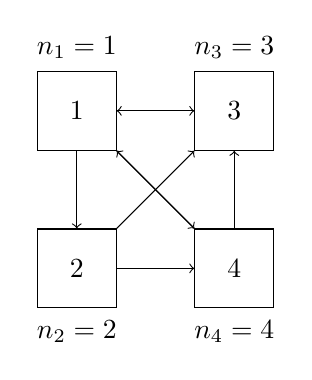
\begin{tikzpicture}
    % Node styles
    \tikzstyle{node_style} = [rectangle, draw, minimum size=1cm]
    
    % Nodes
    \node[node_style] (1) at (0,2) {1};
    \node[node_style] (2) at (0,0) {2};
    \node[node_style] (3) at (2,2) {3};
    \node[node_style] (4) at (2,0) {4};

    % Labels for n values
    \node at (0,2.8) {$n_1 = 1$};
    \node at (0,-0.8) {$n_2 = 2$};
    \node at (2,2.8) {$n_3 = 3$};
    \node at (2,-0.8) {$n_4 = 4$};

    % Arrows
    \draw[->] (1) -- (2);
    \draw[->] (1) -- (3);
    \draw[->] (2) -- (4);
    \draw[->] (4) -- (3);
    \draw[->] (4) -- (1);
    \draw[->] (2) -- (3);
    \draw[->] (3) -- (1);
    \draw[->] (1) -- (4);
\end{tikzpicture}
\end{center}

As shown in the figure, \(n=4, n_{1}=3, n_{2} = 2, n_3 = 1, n_4 = 2, L_{1} = {3,4}, L_{2} = {1}, L_3 = {1,2,4} \text { and } L_4 = {1,2}\). So the formulas for assigning the page rank becomes

\begin{equation}
    \begin{aligned}
        x_{1} &= \frac{x_3}{1} + \frac{x_4}{2} \\
        x_{2} &= \frac{x_{1}}{3} \\
        x_3 &= \frac{x_{1}}{3} + \frac{x_{2}}{2} + \frac{x_4}{2} \\
        x_4 &= \frac{x_{1}}{3} + \frac{x_{2}}{2}.        
    \end{aligned}
\end{equation}

This system of linear equations can be written in vector and matrix notation, as 

\begin{equation}
    A\vb{x} = \vb{x} ,
\end{equation}

where 

\begin{equation}
    \vb{x} = \begin{pmatrix}
         x_{1} \\
         x_{2} \\
         x_3 \\
         x_4  \\
    \end{pmatrix} \text { and } A = \begin{pmatrix}
        0 & 0 & 1 &  \frac{1}{2} \\
        \frac{1}{3} & 0 & 0 & 0  \\
        \frac{1}{3}  & \frac{1}{2}  & 0 & \frac{1}{2}   \\
        \frac{1}{3}  & \frac{1}{2}  & 0 & 0  \\
    \end{pmatrix}.
\end{equation}

This equation describes a so-called ``eigenvalue problem'', which we will discuss in a later stage.}

\section{Vector Spaces} \label{vspace} 

\begin{definition}[Definition of a Vector Space]
A vector space V over a field F is a set with two operations:

\begin{enumerate}
    \item vector addition: \((\vb{v}, \vb{w}) \mapsto \vb{v} + \vb{w} \in V \), where \(\vb{v} , \vb{w} \in V\).
    \item scalar multiplication: \((\alpha ,\vb{v}) \mapsto \alpha \vb{v} \in V\), where \(\alpha \in F \text { and } \vb{v} \in V\). 
\end{enumerate}

And for all \(\vb{u} ,\vb{v} ,\vb{w} \in V\) and all \(\alpha ,\beta \in F\), these operations have to satisfy the following rules:

\begin{enumerate}[label=(\(A\)\arabic*)]\label{vectorspace} 
    \item ``Associativity'': \((\vb{u} + \vb{v} ) + \vb{w}  = \vb{u}  + (\vb{v} + \vb{w} )\).
    \item ``Neutral element'': There exists a ``zero vector'', \(\boldsymbol{0} \in V\) so that \(0 + \vb{v} = \vb{v} \).
    \item ``Inverse element'': There exists an inverse, \(-\vb{v} \) with \(\vb{v} + (-\vb{v} ) = 0\).
    \item ``Commutativity'': \(\vb{v} + \vb{w} = \vb{w} + \vb{v} \).
    \item \(\alpha (\vb{v} +\vb{w} ) = \alpha \vb{v} + \alpha \vb{w} \).
    \item \((\alpha +\beta )\vb{v} = \alpha \vb{v} + \beta \vb{w} \).
    \item \((\alpha \beta )\vb{v} = \alpha (\beta \vb{v} )\).
    \item \(1\cdot \vb{v} = \vb{v} \).
\end{enumerate}

The elements \(\vb{v} \in V\) are called ``vectors'', the elements \(\alpha \in F\) of the field are called ``scalars''.  
\end{definition}

\begin{definition}[Definition of a Sub Vector Space]\label{subvectorspace} 
A sub vector space \(W \subset V \) is a non-empty subset of a vector space \(V\) which is closed under vector addition and scalar multiplication, \textit{i.e.,}\footnote{The rigorous proof of a sub vector space is a vector space itself is provided in \cref{subvectorapp}.} 

\begin{enumerate}[label=(\(B\)\arabic*)]
    \item \(\vb{w} _{1} + \vb{w} _{2} \in W \text{ for all } \vb{w} _{1} , \vb{w} _{2} \in W\).
    \item \(\alpha \vb{w} \in W \text{ for all } \alpha \in \vb{F} \text { and } \vb{w} \in W\).     
\end{enumerate}
\end{definition}

\section{Span and Linear Independence}

\begin{definition}[Definition of Span]
    The span of \(k\) vectors \(\vb{v} _{1} , \ldots , \vb{v} _{k} \) in a vector space \(V\) over a field \(F\) is the set of all linear combinations of all those vectors
\end{definition}

\begin{equation}
    \text{Span} (\vb{v} _{1}, \ldots ,\vb{v} _{k}  ) \equiv  \left\{\sum_{i=1}^{k} \alpha _{i}\vb{v} _{i} \mid  \alpha _{i}\in F    \right\}.
\end{equation}

\begin{definition}[Definition of Linear Independence]
Let \(V\) be a vector space over\(\mathbb{F}\) and \(\alpha _{1}, \ldots , \alpha _{k} \in  F  \) scalars. A set of vectors \(\vb{v} _{1}, \ldots , \vb{v} _{k} \in V\) is called linearly independent if 

\begin{equation}
    \sum_{i=1}^{} \alpha _{i} \vb{v} _{i} = \boldsymbol{0} \implies \alpha _{i} = 0 \text{ for all } i.      
\end{equation}

Otherwise, the vectors are called linearly dependent. 
\end{definition}

\begin{corollary}
The vectors \(\vb{v} _{1}, \ldots , \vb{v} _{k}  \) are linearly dependent \(\iff \) One vector \(\vb{v} _{i} \) can be written as a linear combination of the others. 
\end{corollary}

\begin{proof}
Assume the vectors \(\vb{v} _{1}, \ldots , \vb{v} _{k}  \) are linearly dependent so that the equation \(\sum_{k=1}^{k} \alpha _{i} \vb{v} _{i}  = 0\) has a solution with at least one \(\alpha _{i} \neq 0 \), then we can solve for \(\vb{v} _{i} \) to get

\begin{equation}
    \vb{v} _{i} = -\frac{1}{\alpha _{i} } \sum_{j \neq i}^{} \alpha _{j} \vb{v} _{j} ,    
\end{equation}

where we expressed \(\vb{v} _{i} \) as a linear combination of the other vectors.

\end{proof}


\example{Linear Independence of Vectors in \(\mathbb{R}^3 \).}
{Verify the following vectors in \(\mathbb{R}^3 \) are linearly independent 

\begin{equation}
    \vb{v} _{1} = \begin{pmatrix}
         0 \\
         1 \\
         1 \\
    \end{pmatrix}, \vb{v} _{2} = \begin{pmatrix}
         0 \\
         1 \\
         2 \\
    \end{pmatrix}, \vb{v} _{3} = \begin{pmatrix}
         1 \\
         1 \\
         -1 \\
    \end{pmatrix}, 
\end{equation}}
{Setting the linear combination of vectors to be the zero vector,

\begin{equation}
    \alpha _{1}\vb{v} _{1} + \alpha _{2} \vb{v} _{2} + \alpha _{3} \vb{v} _{3} = \begin{pmatrix}
         \alpha _{3}  \\
         \alpha _{1} + \alpha _{2} + \alpha _{3}   \\
         \alpha _{1} + 2\alpha _{2} - \alpha _{3}   \\
    \end{pmatrix} = \boldsymbol{0} 
\end{equation}

we find that it only has the solution \((\alpha _{1}, \alpha _{2}, \alpha _{3}   ) = (0,0,0)\). Therefore the vectors are linearly independent.
} 

\example{Linear Independence of Trigonometric Functions.}
{Prove that the solutions \(y(x) = \cos x \text { and } y(x) = \sin x\)  to the homogeneous, linear second order differential equation 

\begin{equation}
    \frac{d^2y}{dx^2} = -y
\end{equation}

are linearly indpendent.}
{We start with setting the linear combination of the solutions to 0,

\begin{equation}
    \alpha \sin x+ \beta \cos x= 0,
\end{equation}

and since the equation has to be satisfied for all \(x\),  setting \(x=0\) we learn that \(\beta =0\) and setting \(x=\frac{\pi }{2} \) it follows that \(\alpha = 0\). Hence \(\sin x\) and \(\cos x\)  are linearly independent. 
} 

\example{Linear Dependence of Three Four-Dimensional Vectors.}
{Determine whether the vectors \(\begin{pmatrix}
     1 \\
     2 \\
     0 \\
     -3 \\
\end{pmatrix}, \begin{pmatrix}
     2 \\
     1 \\
     1 \\
     4 \\
\end{pmatrix} \text { and } \begin{pmatrix}
     -3 \\
     6 \\
     -4 \\
     1 \\
\end{pmatrix}\) are linearly indpendent. }
{One way to check their linearly independecy is to check whether setting the linaer combination of them implies that the coefficients of each vector is zero. Alternatively, we can find the rank of the matrix \(A\) formed by the vectors and find its rank. The matrix can be row reduce to

\begin{equation}
    A = \begin{pmatrix}
        1 & 2 &  -3 \\
        2 & 1 &  6 \\
        0 & 1 &  -4 \\
        -3 & -4 &  1 \\
    \end{pmatrix} \to \begin{pmatrix}
        1 & 2 &  -3 \\
        0 & 1 &  -4 \\
        0 & 0 &  0 \\
        0 & 0 &  0 \\
    \end{pmatrix}.
\end{equation}

Therefore the rank of \(A\) is two and the vectors are linearly depedent.
} 


To test whether three three-dimensional vectors are linear indepedence, the fastest way is to compute the determinant and check whether or not it is equals to zero.

\section{Basis and Dimension}
\begin{definition}[Definition of a Basis]
A set \(\vb{v} _{1}, \ldots , \vb{v} _{n} \in V \) of vectors is called a basis of \(V\) if and only if:

\begin{enumerate}[label=(\(C\)\arabic*)] \label{basis} 
    \item \(\vb{v} _{1}, \ldots , \vb{v} _{n}  \) are linearly independent.
    \item \(V = \text{Span}(\vb{v} _{1}, \ldots , \vb{v} _{n}  ) \).
\end{enumerate}
\end{definition}

\begin{lemma} \label{uniquelinear} 
If \(\vb{v} _{1}, \ldots ,\vb{v} _{n}  \) is a basis of \(V\), every vector \(\vb{v} \in V\) can be written as a unique linear combination as

\begin{equation}
    \vb{v} = \sum_{i=1}^{n} \alpha _{i} \vb{v} _{i}  .
\end{equation}

\end{lemma}

\begin{proof}
Firstly we must be able to write \(\vb{v} \) as a linear combination of the basis, since \(\vb{v} \in V \text { and } V = \text{Span} (\vb{v}_1, \cdots, \vb{v}_n ) \).   

Now assume that \(\vb{v} \) can be written as two different linear combinations of the basis, \textit{i.e.,} 

\begin{equation}
    \vb{v} = \sum_{i=1}^{n} \alpha _{i}\vb{v} _{i} = \sum_{i=1}^{n} \beta _{i} \vb{v} _{i}.  
\end{equation}

Taking the difference of these two equations implies

\begin{equation}
    \sum_{i=1}^{n} (\alpha _{i} - \beta _{i}  )\vb{v} _{i} =0
\end{equation}

and from linear independence of the basis, it follows that all \(\alpha _{i} - \beta _{i} = 0  \) for all \(i\), so indeed \(\alpha _{i} = \beta _{i}  \). 
\end{proof}

We would like to call the number of vectors in a basis the dimension of the vector space. First, however, we have to proof that the number of vectors in a basis of a vector space is an invariant.

\begin{lemma}[Exchange Lemma] \label{exchangelemma} 
Let \(\vb{v} _{1}, \ldots , \vb{v} _{n}  \) be a basis of \(V\) and \(\vb{w} _{1}, \ldots ,\vb{w} _{m} \in V \) arbitrary vectors. If \(m > n\) then \(\vb{w} _{1}, \ldots ,\vb{w} _{m}  \) are linearly dependent.  
\end{lemma}

\begin{proof}
Consider the first arbitrary vector \(\vb{w} _{1} \). If \(\vb{w} _{1} = 0 \) then the vectors \(\vb{w} _{1}, \ldots ,\vb{w} _{m}  \) are linearly dependent (since the coefficient of \(\vb{w} _{1} \) can be any arbirary constant when we write down the linaer combination of the vectors \(\vb{w}_1, \cdots, \vb{w}_n \) to test their linear dependency), so we can assume that \(\vb{w} _{1} \neq 0 \).    

Since the vectors \(\vb{v} _{i} \) form a basis we can write the first arbitrary vector as

\begin{equation}
    \vb{w} _{1} = \sum_{i=1}^{n} \alpha _{i} \vb{v} _{i}   
\end{equation}

with at least one \(\alpha _{i}\)  (say \(\alpha _{1} \)) non-zero (or else \(\vb{w} _{1} \) would be zero). We can therefore solve this equation for \(\vb{v} _{1} \) as

\begin{equation}
    \vb{v} _{1} = \frac{1}{\alpha _{1} } \left( \vb{w} _{1} - \sum_{i=2}^{n} \alpha _{i} \vb{v} _{i}   \right). \label{exchangev1} 
\end{equation}

This shows that we use \(\vb{w} _{1} \) to replace \(\vb{v} _{1} \) in basis \(\vb{v}_{1}, \ldots, \vb{v}_n \) such that \(V = \text{Span}(\vb{w} _{1}, \vb{v}_{2}, \ldots, \vb{v}_n  ) \), such that the span is remained unchanged. This is because any vector \(\vb{u} \in V\) which can be written as a linear combination of the basis \(\vb{v}_{1}, \ldots, \vb{v}_n \) can now be written as a linear combination of the basis \(\vb{w} _{1}, \vb{v}_{2}, \ldots, \vb{v}_n \) simply by utilizing \cref{exchangev1}.     

This exchange process can be repeated until all \(\vb{v} _{i} \) are placed by \(\vb{w} _{i} \) and \(V = \text{Span} (\vb{w}_{1}, \ldots, \vb{w}_n ) \). Since \(m > n\) there is at least one vector \(\vb{w} _{n+1} \) ``left over'' which can be written as a lniear combination 

\begin{equation}
    \vb{w} _{n+1} = \sum_{i=1}^{n} \beta _{i} \vb{w} _{i}  
\end{equation}

which shows that the vectors \(\vb{w}_{1}, \ldots, \vb{w}_m\) are linearly dependent.
\end{proof}

\begin{definition}[Definition of Dimension] \label{dimension} 
For a basis \(\vb{v}_{1}, \ldots, \vb{v}_n \) of a vector space \(V\) over\(\mathbb{F}\) we call \(\dim _{F} (V) \equiv n \) the dimension of \(V\) over\(\mathbb{F}\) . 
\end{definition}

\example{Standard Unit Vectors form a Basis.}
{Prove that the standard unit vectors \(\vb{e}_1, \cdots, \vb{e}_n \) form a basis over the vector space \(\mathbb{R}^{n} \text { and } \mathbb{C}^{n} \). }
{Set the linear combination of the standard unit vectors to zero, 

\begin{equation}
    \sum_{i=1}^{n} \alpha _{i} \vb{e} _{i} = \begin{pmatrix}
         \alpha _{1}  \\
         \vdots  \\
         \alpha _{n}  \\
    \end{pmatrix} =0
\end{equation}

which is only true if \(\alpha _{i} = 0 \text{ for all } i\).

Thus the standard unit vectors \(\vb{e}_{1}, \ldots, \vb{e}_n \) form a basis of \(\mathbb{R}^{n} \text { and } \mathbb{C}^{n}  \) seen as vector spaces of the fields \(\mathbb{R}\text { and } \mathbb{C}\), respectively, where the dimensions are 

\begin{equation}
    \dim _{\mathbb{R}} (\mathbb{R}^{n} ) = \dim _{\mathbb{C}} (\mathbb{C}^{n} ) = n. 
\end{equation}

However, note that \(\mathbb{C}^{n} \) as a vector space over \(\mathbb{R}\) has a basis \(\vb{e}_{1}, \ldots, \vb{e}_n, i \vb{e} _{1}, \ldots , i \vb{e} _{n}   \) and therefore \(\dim _{\mathbb{R}} (\mathbb{C}^{n} ) = 2n\). 
} 

\example{Basis of a Polynomial.}
{Prove that the monomials \(1,x,^2,\ldots ,x^{d} \) form a basis over a vector space containing all real polynomials of degree \(d\).}
{We start with setting  
\begin{equation}
    \sum_{i=0}^{d} \alpha _{i} \vb{x} ^{i} =0 
\end{equation}

to check if there is any non-trivial solution. However, by taking the \(k^{\text{th }} \)derivative with respect to \(x\) and then set \(x=0\) (since it has to satisfy for all \(x\)), this immediately implies that \(\alpha _{k} = 0 \text{ for all }  k\) and hence the monomials are linearly independent and form a basis and the vector space has dimension \(d+1\).
}

\example{Basis of a \(n \times m\) matrix.}
{Find a basis and the dimension of the vector space containing all \(n \times m\) matrices with real entries.}
{The analogy of standard unit vectors for matrices is

\begin{equation} \label{matricesbasis} 
    E_{(i,j)}  = \begin{pmatrix}
        0 & \ldots  & 0 & 0 & 0 & \ldots  &  0 \\
        \vdots  &  & \vdots  & \vdots  & \vdots  &  &  \vdots  \\
        0 & \ldots  & 0 & 0 & 0 & \ldots  &  0 \\
        0 & \ldots  & 0 & 1 & 0 & \ldots  &  0 \\
        0 & \ldots  & 0 & 0 & 0 & \ldots  &  0 \\
        \vdots  &  & \vdots  & \vdots  & \vdots  &  &  \vdots  \\
        0 & \ldots  & 0 & 0 & 0 & \ldots  &  0 \\
    \end{pmatrix},\footnote{Here the subscript \((i,j)\) has been used to indicate the row and column which have been changed rather than specific entries of the matrix. } 
\end{equation}

where \(i=1,\ldots ,n \text { and } j= 1,\ldots ,m\) and the ``1'' appears in the \(i^{\text{th }} \)row and the \(j^{\text{th }} \)column with all other entries zero. Clearly these matrices form a basis, in complete analogy with the standard unit vectors. Therefore the vector space of \(n\times m\) matrices has dimension \(nm\).    
} 

\begin{lemma}[Properties of a Vector Space]
For a vector sapce \(V\) spanned by a finite number of vectors we have:

\begin{enumerate}[label=(\(D\)\arabic*)] 
    \item \(V \) has a basis.
    \item Every linearly independent set \(\vb{v}_{1}, \ldots, \vb{v}_k \in V\) that is not already a basis of \(V\) can be completed by some other vectors in \(V\) to form a basis.
    \item If \(n = \dim (V)\), any linaerly independent set of vectors \(\vb{v}_{1}, \ldots, \vb{v}_n \) forms a basis.
    \item If \(\dim _{F} (V) = \dim _{F} (W)\) and \(V \subset W\) for two vector spaces \(V \text { and } W\) then \(V=W\).      
\end{enumerate}

\end{lemma}

\begin{proof}

\begin{enumerate}[label=(\(D\)\arabic*)] 
    \item Since \(V = \text{Span}(\vb{v}_{1}, \ldots, \vb{v}_k ) \), If these vectors are linearly independent we have found a basis. If not, one of the vectors, say \(v_{k} \) can be written as a linear combination of the others and can, hence, be dropped without changing the spoan, so \(V = \text{Span}(\vb{v}_{1}, \ldots, \vb{v}_{k-1}) \). This process can be continued until the remainng set of vectors is linaerly independent.
    \item If \(V= \text{Span}(\vb{v}_{1}, \ldots, \vb{v}_k) \) we are finished. If not there exists a vector \(\vb{v} _{k+1} \notin Span(\vb{v}_{1}, \ldots, \vb{v}_k) \). Hence the vectors \(\vb{v}_{1}, \ldots, \vb{v}_k, \vb{v} _{k+1} \) must be linaerly independent. We can continue adding vectors to the list until it spans the whole space. This process must terminate after a finite number of steps or else we would contradict the exchange \cref{exchangelemma}, which states that the number of vectors in a basis is an invariant.
    \item If \(\dim (V) = n\) and the linearly independent set \(\vb{v}_{1}, \ldots, \vb{v}_n \) did not span \(V\) then from (D2) it could be completed to a basis with more than \(n\) elements. However this is a contradiction since according to the exchange \cref{exchangelemma} the number of vectors in a basis is an invariant. So the vectors \(\vb{v}_{1}, \ldots, \vb{v}_n \) must span the space and they form a basis.
    \item We can choose a basis \(\vb{v}_{1}, \ldots, \vb{v}_n \) of V. Since \(V \subset W\), these basis vectors are linaerly independent in \(W\), and since \(\dim _{F} (W) = \dim _{F} (V)  \), they must also form a basis of \(W\), using (D3). Hence \(V = \text{Span}(\vb{v}_{1}, \ldots, \vb{v}_n ) = W \).         
\end{enumerate}

\end{proof}

\todo{magic square} 

\chapter{Geometrical Applications of Vectors in \(\mathbb{R}^{n} \)}

\section{Scalar and Vector Products}

\subsection{Kronecker Delta and Levi-Civita Symbol}

The kronecker delta is defined by 

\begin{equation}
\delta_{ij} =
\begin{cases} 
1 & \text{if } i = j, \\
0 & \text{if } i \neq j.
\end{cases}
\end{equation}

The Levi-Civita symbol is defined by 

\begin{equation}
    \epsilon_{ijk} =
\begin{cases} 
+1 & \text{if } (i, j, k) = (1, 2, 3), (2, 3, 1), (3, 1, 2), \\
-1 & \text{if } (i, j, k) = (2, 1, 3), (3, 2, 1), (1, 3, 2), \\
~0 & \text{otherwise}.
\end{cases}
\end{equation}

In Einstein summation convention, there is are pairs of dummy indices and some free indices. The free indices indicate which component of the vector we are describing, and only appear once in a term, but there can be more than one free indices. The repeated (twice) indices are the dummy indices, which implies summation over them. No indices can appear more than twice. 

Note, however, for example, that \(x_{i}^2 \neq x_{i}x_{i}   \) when we use the Einstein summation convention. The former is the square of the \(i^{\text{th }} \) component of the vector \(\vb{x} \), and the latter is summing over the square of all components of the vector \(\vb{x} \).    

One important equality regarding the Levi-Civita Symbol is 

\begin{equation}
    \epsilon _{ijk}\epsilon _{ilm} = \delta _{jl}\delta _{km} - \delta _{jm}\delta _{kl},      
\end{equation}

which is true, since \(\epsilon _{ijk}\epsilon _{ilm} = \sum_{i=1}^{3} \epsilon _{ijk}\epsilon _{ilm} = +1  \) if \((j,l) = (k,m)\) and \(\epsilon _{ijk} = -1 \) if \((j,l) = (m,k)\) (and in any other combinations of \((j,k,l,m)\) we get zero).

\subsection{Scalar Product in \(\mathbb{R}^{n} \) }

The scalar (dot) product for two n-demensional column vectors is defined as

\begin{equation}
    \vb{a} \cdot \vb{b} \equiv \sum_{i=1}^{n} a_{i} b_{i} = a_{i}b_{i} = \delta _{ij}a_{i}b_{j},    
\end{equation}

given that the basis is orthogonal. (The dot product for under a general basis will be covered in \cref{dot}).

The dot product satisfies a number of obvious properties, namely

\begin{enumerate}
    \item \(\vb{a} \cdot \vb{b} = a_{i} b_{i} = b_{i} a_{i} = \vb{b} \cdot \vb{a}  \)
    \item \(\vb{a} \cdot (\vb{b} + \vb{c} ) = a_{i} (b_{i} + c_{i}  ) = a_{i}b_{i} + a_{i}c_{i}   = \vb{a} \cdot \vb{b} + \vb{a} \cdot \vb{c}  \)
    \item \(\vb{a} \cdot (\beta \vb{b} ) = a_{i}(\beta b_{i} ) = \beta a_{i}b_{i} = \beta \vb{a} \cdot \vb{b}    \)
    \item \(\vb{a} \cdot \vb{a}  = \sum_{i=1}^{n} a_{i}^2 > 0 \text{ for } \vb{a} \neq \boldsymbol{0}  \)
\end{enumerate}

The last property allows us to define the length of a vector as 

\begin{equation}
    \abs{\vb{a} } \equiv \sqrt{\vb{a} \cdot \vb{a} } = \left( \sum_{i=1}^{n} a_{i}^2  \right) ^{\frac{1}{2} } 
\end{equation}

given that the basis is orthogonal.

\begin{lemma}[Cauchy-Schwarz inequality]
For any two vectors \(\vb{a} \) and \(\vb{b} \) in \(\mathbb{R}^{n} \) we have

\begin{equation}
    \abs{\vb{a} \cdot \vb{b} } \le \abs{\vb{a} }\abs{\vb{b} }.  
\end{equation}

\end{lemma}

\begin{proof}
Without loss of generality let \(\abs{\vb{a} } = \abs{\vb{b} } = 1  \) (if this is not the case then we can always normalize the vectors). Then

\begin{equation}
    0 \le \abs{\vb{a} \pm \vb{b} }^2 = (\vb{a} \pm \vb{b} )\cdot (\vb{a} \pm \vb{b} ) = \abs{\vb{a} }^2 + 2(\vb{a} \cdot \vb{b} ) + \abs{\vb{b} }^2 = 2(1 \pm \vb{a} \cdot \vb{b} ) \implies \abs{\vb{a} \cdot \vb{b} } \le 1. 
\end{equation}
\end{proof}

A closely related inequality is the famous

\begin{lemma}[Triangle Inequality]
For any two vectors \(\vb{a} \text { and } \vb{b} \) in \(\mathbb{R}^{n} \) we have

\begin{equation}
    \abs{\vb{a} + \vb{b} } \le \abs{\vb{a} } + \abs{\vb{b} }   
\end{equation}
\end{lemma}

\begin{proof}
\(\abs{\vb{a} +\vb{b} }^2 = \abs{\vb{a} }^2 + \abs{\vb{b} }^2 + 2 \vb{a} \cdot \vb{b} \le \abs{\vb{a} }^2 + \abs{\vb{b} }^2 + 2\abs{\vb{a} }\abs{\vb{b} } = (\abs{\vb{a} } + \abs{\vb{b} }  )^2      \). 
\end{proof}

For two non-zero vectors \(\vb{a} \text { and } \vb{b} \), the Cauchy-Schwarz inequality implies that we can define an unique angle \(\theta \in [0,\pi ]\) as

\begin{equation}
    -1 \le \cos \theta = \frac{\vb{a} \cdot \vb{b} }{\abs{a}\abs{b}  } \le 1 \implies \vb{a} \cdot \vb{b} = \abs{\vb{a} } \abs{\vb{b} }\cos \theta .  
\end{equation}

We call two vectors orthogonal (or perpendicular) if and only if \(\vb{a} \cdot \vb{b} = 0, \text { or }  \theta = \frac{\pi }{2} \).

\subsection{Vector Product in \(\mathbb{R}^3 \) }
	
\subsubsection{Scalar Triple Product \(\vb{A} \cdot (\vb{B} \cross \vb{C})\)}
	
The scalar triple product \(\vb{A} \cdot (\vb{B} \cross \vb{C})\) represents the volume of the parallelepiped generated by \(\vb{A}\), \(\vb{B}\) and \(\vb{C}\) (as shown in \cref{para}) since \(\abs{\vb{B} \cross \vb{C}}\) is the base area, and \(\abs{\vb{A}\cos{\theta}}\) is the altitude. Therefore, by considering different pairs of bases and altitudes, the following identity can be shown
	
\begin{equation} 
  \vb{A} \cdot (\vb{B} \cross \vb{C}) = \vb{B} \cdot (\vb{C} \cross \vb{A}) = \vb{C} \cdot (\vb{A} \cross \vb{B}). \label{scatri} 
\end{equation}
	
An easy way to remember this identity is that it adopts the same ``clockwise convention'' as \(\vu{x} \cross \vu{y} = \vu{z} ~  \&  ~ \vu{y} \cross \vu{z} = \vu{x} ~  \&  ~ \vu{z} \cross \vu{x} = \vu{y}\).
	
\onefig{para}{scale=0.3}

\subsubsection{Vector Triple Product \(\vb{A} \cross (\vb{B} \cross \vb{C})\)}
	
The vector triple product \(\vb{A} \cross (\vb{B} \cross \vb{C})\) can be simplified with the so-called \(\vb{BAC-CAB}\) identity
	
\begin{equation} 
	\vb{A} \cross (\vb{B} \cross \vb{C}) = \vb{B}(\vb{A} \cdot \vb{C}) - \vb{C}(\vb{A} \cdot \vb{B}). \label{vectri} 
\end{equation}		

This can be shown by 

\begin{equation}
    \begin{aligned} 
    \left( \vb{a} \cross (\vb{b} \cross \vb{c} ) \right)_{i} &= \epsilon _{ijk}a_{j}\left( \vb{b} \cross \vb{c}  \right)_{k} \\
    &= \epsilon _{ijk} a_{j}\epsilon _{kmn}b_{m}c_{n} \\
    &= (\delta _{im}\delta _{jn}-\delta _{in}\delta _{jm}) a_{j}b_{m}c_{n} \\
    &= a_{j}b_{i}c_{j}- a_{j}b_{j}c_{i} \\
    &= \left((\vb{a} \cdot \vb{c} )\vb{b} - (\vb{a} \cdot \vb{b} )\vb{c}\right)_{i}               
    \end{aligned} 
\end{equation}


	
With \cref{scatri} and \cref{vectri} in hand, it is never necessary for an expression to contain more than one cross product in any term.
	
\example
{Griffiths (5th ed.) P.8}
{Simplify \((\vb{A} \cross \vb{B}) \cdot (\vb{C} \cross \vb{D})\) and \(\vb{A} \cross (\vb{B} \cross (\vb{C} \cross \vb{D}))\).}
{For the first equality, using \cref{scatri,vectri}, we have 
\begin{equation} 
	\begin{aligned} 
		(\vb{A} \cross \vb{B}) \cdot (\vb{C} \cross \vb{D}) &= \vb{C} \cdot (\vb{D} \cross (\vb{A} \cross \vb{B})) \\ 
			&= \vb{C} \cdot (\vb{A}(\vb{B} \cdot \vb {D}) - \vb{B}(\vb{D} \cdot \vb{A}))  \\
			&= (\vb{A} \cdot \vb{C})(\vb{B} \cdot \vb{D}) - (\vb{A} \cdot \vb{D})(\vb{B} \cdot \vb{C}).
	\end{aligned} 
\end{equation}

Alternatively, we have

\begin{equation}
    \begin{aligned} 
    ((\vb{a} \cross \vb{b} )\cdot (\vb{c} \cross \vb{d} ))_{i} &= (\vb{a} \cross \vb{b} )_{i} (\vb{c} \cross \vb{d} )_{i} \\
    &= \epsilon _{ijk}a_{j} b_{k}\epsilon _{imn}c_{m}d_{n} \\
    &= \epsilon _{jki}\epsilon _{imn} a_{j} b_{k} c_{m} d_{n} \\
    &= (\delta _{jm} \delta _{kn} - \delta _{jn} \delta _{mk} ) a_{j} b_{k} c_{m} d_{n} \\
    &= a_{j} c_{j} b_{k} d_{k} - a_{j} d_{j} b_{k} c_{k} \\
    &= (\vb{a} \cdot \vb{c} )(\vb{b} \cdot \vb{d} ) -  (\vb{a} \cdot \vb{d} )(\vb{b} \cdot \vb{c} ).         
    \end{aligned} 
\end{equation}

For the second equality,

\begin{equation} 
	\begin{aligned} 
		\vb{A} \cross (\vb{B} \cross (\vb{C} \cross \vb{D})) &= \vb{A} \cross(\vb{C}(\vb{B} \cdot \vb{D}) - \vb{D}(\vb{B} \cdot \vb{C}))  \\
			&= (\vb{B} \cdot \vb{D})(\vb{A} \cross \vb{C}) - (\vb{B} \cdot \vb{C})(\vb{A} \cross \vb{D}) \\
			(\text { or }  ~ \vb{A} \cross (\vb{B} \cross (\vb{C} \cross \vb{D})) &= \vb{B}(\vb{A} \cdot (\vb{C} \cross \vb{D})) - (\vb{C} \cross \vb{D})(\vb{A} \cdot \vb{B}))
	\end{aligned} 
\end{equation}}

\example
{Griffiths (5th ed.) Problem 1.6}
{When does \(\vb{A} \cross (\vb{B} \cross \vb{C})\) = \((\vb{A} \cross \vb{B}) \cross \vb{C}\)?}
{Since
\begin{equation}
	\begin{aligned}
		&\vb{A} \cross (\vb{B} \cross \vb{C}) + \vb{B} \cross (\vb{C} \cross \vb{A}) + \vb{C} \cross (\vb{A} \cross \vb{B}) \\
		= ~&\vb{B}(\vb{A} \cdot \vb{C}) - \vb{C}(\vb{A} \cdot \vb{B}) + (\vb{C}(\vb{B} \cdot \vb{A}) - \vb{A}(\vb{B} \cdot \vb{C})) + (\vb{A}(\vb{C} \cdot \vb{B}) - \vb{B}(\vb{C} \cdot \vb{A})) \\
		= ~&0,
	\end{aligned}
\end{equation}

Therefore, \(\vb{A} \cross (\vb{B} \cross \vb{C}) = (\vb{A} \cross \vb{B}) \cross \vb{C}\) when \(\vb{B} \cross (\vb{C} \cross \vb{A}) = 0\).

Thus, either \(\vb{A} \parallelsum \vb{C} ~ or ~ \vb{A} \perp \vb{B} \perp \vb{C}\)}

\example{Quadraple Cross Product.}
{Simplify \((\vb{a} \cross \vb{b} )\cross (\vb{c} \cross \vb{b} )\). }
{\begin{equation}
    \begin{aligned}
        ((\vb{a} \cross \vb{b} )\cross (\vb{c} \cross \vb{b} ))_{i}  &= \epsilon _{ijk} (\epsilon _{jpq} a_{p} b_{q} )(\epsilon _{krs} c_{r} b_{s} ) \\
        &= \epsilon _{ijk} \epsilon _{krs} \epsilon _{jpq} a_{p} b_{q} c_{r} b_{s} \\
        &= (\delta _{ir} \delta _{js} -\delta _{is} \delta _{rj} ) \epsilon _{jpq} a_{p} b_{q} c_{r} b_{s} \\
        &= \epsilon _{jpq} a_{p} b_{q} (c_{i} b_{j} -b_{i} c_{j} ) \\
        &= ((\vb{a} \cross \vb{b} )\cdot \vb{b} )c_{i} - ((\vb{a} \cross \vb{b} )\cdot \vb{c} )b_{i} \\
        &= (\vb{b} \cdot (\vb{a} \cross \vb{c} ))b_{i}.  
    \end{aligned}
\end{equation}

} 


\section{Equations of Lines, Planes and Spheres}

\subsection{Equation of Lines}

The general equation of a line is 

\begin{equation}
    \vb{r} = \vb{a} + \lambda \vb{b} \Longleftrightarrow (\vb{r} - \vb{a} ) \cross \vb{b} = \boldsymbol{0} \Longleftrightarrow \frac{x-a_{x} }{b_{x} } = \frac{y - a_{y} }{b_{y} } = \frac{z - a_{z} }{b_{z} } = \text{constant}, 
\end{equation}

where \(\vb{r} \) is the position vector of a general point on the line, \(\vb{a} \) is the position vector of some fixed point on the line and \(\vb{b} \) is some fixed vector along the direction of the line.   

\subsection{Equation of Planes}

The general equation of a plane is 

\begin{equation}
    \vb{r} = \vb{a} + \lambda \vb{b} + \mu \vb{c} \Longleftrightarrow (\vb{r} - \vb{a} ) \cdot \vu{n} = \boldsymbol{0} \Longleftrightarrow \vb{r} \cdot \vu{n} = \hat{n}_{x} x + \hat{n}_{y} y + \hat{n}_{z} z = \text{constant} , 
\end{equation}

where \(\vb{a} \) is the position vector of some fixed point on the plane, \(\vb{b} \text { and } \vb{c} \) are some fixed (linearly independent) vectors along the direction of the plane and \(\vu{n}\) is the normal vector of the surface. 

\example{Line of Intersection of Two Planes.}
{Find the direction of the line of intersection of the two planes \(x+3y-z=5 \text { and } 2x-2y+4z=3\). }
{The two planes have normal vectors \(\vu{n} _{1} = \vu{x} + 3\vu{y} -\vu{z} \text { and } \vu{n} _{2} = 2\vu{x} -2\vu{y} + 4\vu{z}   \). The direction of the intersecting line mst be parallel to both planes and hence perpendicular to both normals. Therfore, \(\vb{p} = \vu{n} _{1}\cross \vu{n} _{2} = 10\vu{x}-6\vu{y} -8\vu{z}   \). } 

The general equation of a sphere is 

\begin{equation}
    \abs{\vb{r} - \vb{c} }^2 = a^2, 
\end{equation}

where \(\vb{c} \) is the position vector of the center of the sphere and \(a\) is the radius of the sphere.

\example{Planes and Spheres.}
{Find the radius \(\rho \) of the circle that is the intersection of the plane \(\vu{n} \cdot \vb{r} = p\) and the sphere of radius \(a\) centered on the point with position vector \(\vb{c} \).}
{The equation of the sphere is 

\begin{equation}
    \abs{\vb{r} - \vb{c} }^2= a^2 \implies r^2 - 2\vb{r} \cdot \vb{c} +c^2= a^2, 
\end{equation}
    
while the equation of the circle of intersection is 

\begin{equation}
    \abs{\vb{r} - \vb{b} }^2 = \rho ^2, 
\end{equation}

where \(\vb{r} \) is restricted to lie in the plane and \(\vb{b} \) is the position vector of the circle's center.

From simple geometry, we have

\begin{equation}
    \vb{b} - \vb{c} = \lambda \vu{n} ~\text { and }~ \rho ^2 + \abs{\vb{b} -\vb{c} }^2 = a^2, 
\end{equation}

which gives \(\vb{b} = \vb{c} + \sqrt{a^2-\rho ^2}\vu{n}  \). Substituting into the the equation of the circle, we have

\begin{equation}
    r^2- 2\vb{r} \cdot \left( \vb{c} + \sqrt{a^2- \rho ^2} \vu{n}  \right) + c^2 + 2(\vb{c} \cdot \vu{n} )\sqrt{a^2-\rho ^2}+a^2-\rho ^2 = \rho ^2.
\end{equation}

We finally yields \(\rho = \sqrt{a^2- (p-c \cdot \vu{n} )^2} \). 

} 

\section{Distances Between Points, Lines and Planes}

\subsection{Distances From a Point to a Line}

The minimum distance \(d\) from a point \(P\) with position vector \(\vb{p} \) to the line \(\vb{r} = \vb{a} + \lambda \vb{b} \) is given by 

\begin{equation}
    d = \abs{\vb{p} -\vb{a} }\sin \theta = \abs{(\vb{p} -\vb{a} )\cross \vu{b}  }. 
\end{equation}

\subsection{Distances From a Point to a Plane}

The minimum distance \(d\) from a point \(P\) with position vector \(\vb{p} \) to the plane \((\vb{r} - \vb{a} )\cdot \vu{n} = 0\)  is given by 

\begin{equation}
    d = \abs{\vb{p} - \vb{a} }\sin \theta = \abs{\vb{p} - \vb{a} }\cdot \vu{n} .  
\end{equation}

Note that the sign of \(d\) indicate whether the point \(P\) is on the same or opposite side of the surface as the origin. 

\subsection{Distances From a Line to a Line}

Consider two lines \(\vb{r} = \vb{a} + \lambda \vb{a}' \text { and } \vb{r} ' = \vb{b} + \mu '\vb{b} '\). To find the minimum distance \(d\) between the two lines, it is easier to imagine two parallel planes, each consists of one of the lines.

The common normal unit vector of the two planes is 

\begin{equation}
    \vu{n} = \frac{\vb{b} \cross \vb{a} }{\abs{\vb{b} \cross \vb{a} } }, 
\end{equation}

and the minimum distance \(d\) is 

\begin{equation}
    d = \abs{\vb{b} \cross \vb{a} } \sin \theta = \abs{(\vb{b} \cross \vb{a} )\cdot \frac{\vb{b} \cross \vb{a} }{\abs{\vb{b} \cross \vb{a} } }} .
\end{equation}

\subsection{Distances From a Line to a Plane}

The minimum distance \(d\) from a line \(\vb{r} = \vb{a} + \lambda \vb{b} \) to a plane \((\vb{r}' - \vb{a} ')\cdot \vu{n} \) is always zero unless the line is parallel to the plane (\textit{i.e.,} \(\vb{b} \cdot \vu{n} = 0\)). In those cases, the minimum distance \(d\) is 

\begin{equation}
    d = \abs{(\vb{r} ' - \vb{a} ) \cdot \vu{n} }. 
\end{equation}

\subsection{Ratio Theorem}

Let \(\vb{a} \text { and } \vb{b} \) be the position vectors of point \(A \text { and } B\) respectively. If point \(P\) with position vector \(\vb{p} \) divides the line segement \(AB\) in the ratio \(\lambda : \mu \), then \(\vb{p} \) is given by 

\begin{equation}
    \vb{p} = \frac{\mu \vb{a} + \lambda \vb{b} }{\mu + \lambda }. 
\end{equation}

\example{Position Vector of the Centroid of a Triangle.}
{The vertices of triangle \(ABC\) have position vectors \(\vb{a} ,\vb{b} \text { and } \vb{c} \) (refer to \cref{centroid}). Find the position vector of the centroid \(G\) of the triangle.}
{The position vectors of \(D \text { and } E\) are 

\begin{equation}
    \vb{d} = \frac{\vb{a} }{2} + \frac{\vb{b} }{2} ~\text { and }~ \vb{e} = \frac{\vb{a} }{2} + \frac{\vb{c} }{2}.    
\end{equation}

A general point on \(CD\) that divides the line in the ratio \(\lambda : 1- \lambda \) has the position vector 

\begin{equation}
    \vb{r} = (1-\lambda )\vb{c} + \lambda \vb{d} = (1-\lambda )\vb{c} + \frac{\lambda }{2} (\vb{a} +\vb{b} ). 
\end{equation}

Similarly, a general point on \(BE\) that divides the line in the ratio \(\mu :1-\mu \) can be expressed as 

\begin{equation}
    \vb{r} = (1-\mu )\vb{b} + \mu \vb{e} = (1-\mu )\vb{b} + \frac{\mu }{2}(\vb{a} + \vb{c} ). 
\end{equation}

Thus at \(G\), which is the intersection of \(CD \text { and } BE\), we require

\begin{equation}
    (1-\lambda )\vb{c} + \frac{\lambda }{2}(\vb{a} +\vb{b} ) = (1-\mu )\vb{b} + \frac{\mu }{2}(\vb{a} +\vb{c} ).
\end{equation}

Equating the coefficients, we have

\begin{equation}
    \lambda = \mu , \frac{\lambda }{2} = 1-\mu ~\text { and }~ 1-\lambda = \frac{\mu }{2} \implies \vb{g} = \frac{1}{3}(\vb{a} +\vb{b} +\vb{c} ). 
\end{equation}







} 

\onefig{centroid}{scale=0.3} 

\section{Reciprocal Vectors}

The two sets of vectors \(\vb{a} ,\vb{b}, \vb{c} \) and \(\vb{a} ', \vb{b} ', \vb{c} '\) are called reciprocal sets if \(\vb{a} \cdot \vb{a} ' = \vb{b} \cdot \vb{b} ' = \vb{c} \cdot \vb{c} ' = 1\) while other possible combinations of dot product is zero. 

They are related by 

\begin{equation}
    \vb{a} ' = \frac{\vb{b} \cross \vb{c} }{\vb{a} \cdot (\vb{b} \cross \vb{c} )} = \frac{\vb{b} \cross \vb{c} }{\det (\vb{a} , \vb{b} , \vb{c} )}, \quad \vb{b} ' = \frac{c \cross \vb{a} }{\det (\vb{a} ,\vb{b} ,\vb{c} )} ~\text { and }~ \vb{c} '= \frac{\vb{a} \cross \vb{b} }{\det (\vb{a} ,\vb{b} ,\vb{c} )}.   
\end{equation}

If \(\vb{a} ,\vb{b} ,\vb{c} \) are mutually orthogonal then \(\vb{a} ' = \vb{a} , \vb{b} ' = \vb{b} \text { and } \vb{c} '=\vb{c} \).  

The reciprocal vectors are useful, since the components of an arbitrary vector can be represented by a dot product, similar to how for an orthogonal basis, we have \(\vb{v} = \sum_{i=1}^{n} (\vb{v} \cdot \vb{e} _{i}  ) \vb{e} _{i}  \), but for non-orthogonal basis we replace \(\vb{e} _{i}\) by \( \vb{e} _{i}'  \), so \(\vb{v} = \sum_{i=1}^{n} v_{i}\vb{e} '_{i}  \). This is because

\begin{equation}
    \vb{v} \cdot \vb{e} '_{i} = \sum_{i=1}^{n} v_{i} \vb{e} _{i} \cdot \vb{e} '_{i} = v_{i}.       
\end{equation}







\chapter{Linear Maps and Matrices}

\section{Maps and Sets}

\begin{definition}[Definition of a Map]
A map between two sets \(X \text { and } Y\) assigns to each \(x \in  X \) a \(y \in Y\) which is written as \(y=f(x)\) and referred to as the image (or range) of \(x\) under \(f\). In symbols, 

\begin{equation}
    f:X \rightarrow Y,~~~  x \mapsto f(x).
\end{equation}

The set \(X\) is called the domain of the map \(f\) , \(Y\) is called the co-domain of \(f\). The set 

\begin{equation}
    \Im (f) = \left\{ f(x) \mid x \in  X \right\} \subseteq Y
\end{equation}

is called the image of \(f\) and consists of all elements of the co-domain which can be obtained as images under \(f\). 


\end{definition}

\begin{definition}[Terminology for Maps]
Let \(f:X \rightarrow Y\) be a map between two sets \(X \text { and } Y\). The map \(f\) is called

\begin{enumerate}
    \item Injective: if every element of the co-domain is the image of at most one element of the domain. Mathematically,
    
    \begin{equation}
        f(x) = f(\tilde{x} ) \implies x = \tilde{x} \text{ for all } x,\tilde{x} \in X.
    \end{equation}

    \item Surjective: if every element of the co-domain is the image of at least one element of the domain. Mathematically,
    
    \begin{equation}
        \Im (f) = Y
    \end{equation}
    
    \item Bijective: if it is injective and surjective, \textit{i.e.,} if every element of the co-domain is the image of precisely one element of the domain.
   
\end{enumerate}

\end{definition}

\begin{definition}[Definition of a Composite Map]
For two maps \(f:X \rightarrow Y \text { and } g: Y \rightarrow Z\) the composite map  \(g \circ f: X \rightarrow Z\) is defined by

\begin{equation}
    (g \circ f)(x) \equiv g(f(x))
\end{equation}

\end{definition}

From this definition it is easy to show that map composition is associative

\begin{equation}
    h \circ (g \circ  f) = (h \circ  g) \circ f
\end{equation}

since \((h \circ (g \circ f))(x) = h((g \circ f)(x)) = h(g(f(x))) = (h \circ g)(f(x)) = ((h \circ g) \circ f)(x)\).

\begin{definition}[Definition of an Identity Map]
A identity map \(\mathrm{id}_{X} : X \rightarrow X\)  maps every element in \(X\) onto itself, \textit{i.e.,} 

\begin{equation}
    \mathrm{id}_{X} (x) = x \text{ for all } x \in  X.
\end{equation}
\end{definition}

\begin{definition}[Definition of an Inverse Map]
Given a map \(f: X \rightarrow Y\), a map \(g: Y \rightarrow X\) is called an inverse of \(f\) if

\begin{equation}
    (g \circ  f) = \mathrm{id}_{X} \text { and } (f \circ g) = \mathrm{id}_{Y}. 
\end{equation}

\end{definition}

\begin{theorem} [Relation between Inverse and Bijective Maps]\label{bijectiveinverse} 
The map \(f: X \rightarrow Y\) has an inverse if and only if \(f\) is bijective. If the inverse exists it is unique and denoted by \(f^{-1} : Y \rightarrow X\). 
\end{theorem}

\begin{proof}
    If the map is not surjective, an inverse map could not exist since some \(y\) are not in the image of \(f\). If the map is not injective, an inverse map could not exist as well since some \(y \in  Y\) are the images of more than one element in the domain.\footnote{The rigorous proof of this theorem can be found in \cref{bijectiveinverseapp}.}
\end{proof}

\begin{theorem} [Inverse of a Composite Map] \label{compositeinversetheo} 
If the maps \(f: X \rightarrow Y\) and \(g: Y \rightarrow Z\) are both bijective, then the composite map \(f \circ g: Y \rightarrow Z\) is also bijective and hence by \cref{bijectiveinverse} has an inverse given by\footnote{The theorem is intuitive and trivial but the rigorous proof is given in \cref{compositeinverseapp}.}

\begin{equation} \label{compositeinverseeq} 
    (f \circ g)^{-1} = g^{-1} \circ f^{-1} 
\end{equation}

\end{theorem}


\section{Linear Maps}

\begin{definition}[Definition of a Linear Map] \label{linearmap} 
A map \(f:V \rightarrow W\) between two vector spaces \(V \text { and }  W\) over a field \(F\) is called linear if:

\begin{enumerate}[label=(\(E\)\arabic*)]
    \item \(f(\vb{v} _{1} + \vb{v} _{2}  ) = f(\vb{v} _{1} ) + f(\vb{v} _{2} )\).
    \item \(f(\alpha \vb{v} ) = \alpha f(\vb{v} )\).
\end{enumerate}

for all \(\vb{v} ,\vb{v} _{1}, \vb{v} _{2}\in V  \) and for all \(\alpha \in  F\). 

\end{definition}

\begin{definition}[Definition of Kernel]
For a map \(f: V \rightarrow W\), the subset of \(V\) which consists of all vectors \(\vb{v} \in V\) mapped to the zero vector, is defined as the kernel (or null space) of the map \(\ker (f)\). Mathematically,
    
\begin{equation}
    \ker (f) = \left\{ \vb{v} \in V \mid f(\vb{v} )=0 \right\} \subset V.
\end{equation}
    
\end{definition}

\begin{lemma}[Properties of a Linear Map (1)] \label{linearmapprop1} 
A linaer map \(f:V \rightarrow W\) between two vector spaces \(V \text { and }  W\) over\(\mathbb{F}\) has the following properties:\footnote{Since the properties are rather intuitive and trivial, the rigorous proof for these properties is provided in \cref{linearmapprop1app}.} 

\begin{enumerate}[label=(\(F\)\arabic*)]
    \item The zero vectors are mapped onto each other, so \(f(\boldsymbol{0} ) = 0\). Hence \(\boldsymbol{0} \in \ker (f) \).
    \item The kernel of \(f\) is a sub vector space of V.
    \item The image of \(f\) is a sub vector space of \(W\) .
    \item \(f\) is surjective \(\iff \Im (f) = W \iff \dim \Im (f) = \dim (W)\)
    \item \(f\) is injective \(\iff \ker (f) = \left\{ \boldsymbol{0}  \right\} \iff \dim \ker (f) = 0\)
    \item The scalar multiple \(\alpha f\), where \(\alpha \in  F\), is linear.
    \item For another linear map \(g: V \rightarrow W\), the sum \(f+g\) is linear.
    \item For another linear map \(g: W \rightarrow  U\), the composition \(g \circ f\) is linear.\footnote{From (F7) and (F8), since the scalar multiple of a linear map and the sum of two linear maps is again a linear map, the set of linear maps does indeed form a vector space iteself, denoted \(\text{Hom}(V,W)\), called the homomorphisms from \(V\) to W.}
\end{enumerate}
\end{lemma}

\begin{definition}[Definition of Rank] 
The dimension of the image of a linear map \(f\) is called the rank of \(f\). In symbols,

\begin{equation}
    \rank (f) \equiv \dim \Im (f).
\end{equation}
    
\end{definition}

To be concrete, consider a linear map \(f:\mathbb{R}^3 \rightarrow \mathbb{R}^2\) and assume that \(\dim \ker (f) = 2\), \textit{i.e.,} the kernel of \(f\) is a plane in \(\mathbb{R}^3 \) (which passes through the origin since any sub vector space contains the zero vector). Now consider two vectors \(\vb{v} _{1}  ,\vb{v} _{2}  \in \ker (f) + \vb{k}  \) which both lie in a plane parallel to \(\ker (f)\), shifted by a vector \(\vb{k} \). Then we have \(\vb{v} _{1} - \vb{v} _{2} \in \ker (f) \) so that \(f(\vb{v} _{1} - \vb{v} _{2} )=0\) and, hence, by linearity \(f(\vb{v} _{1} ) = f(\vb{v} _{2} )\). Therefore, not only do all vectors in the kernel get mapped to the zero vector, but all vectors in a plane parallel to the kernel get mapped to the same non-zero vector. Effectively, the action of the linear map ``removes '' the two dimensions parallel to the kernel plane and only keeps the remaining dimension perpendicular to it. Hence, the image of this linear map is one-dimensional, which is a line through the origin. This example suggests the following theorem:

\begin{theorem}[Dimension Formula]\label{dimensionformulatheo}
For a linear map \(f:V \rightarrow  W\) we have

\begin{equation}
    \dim \ker (f) + \rank (f) = \dim (V).\footnote{Since this formula is relatively intuitive and imaginable, the rigorous proof is given in \cref{dimensionformulaapp}.} \label{dimensionformulaeq} 
\end{equation}

\end{theorem}

\begin{lemma}[Properties of a Linear Map (2)]\label{linearmapprop2} 
For a linaer map \(f:V \rightarrow W\) we have:\footnote{The rigorous proof is given in \cref{linearmapprop2app} due to its simplicity and imaganability.} 

\begin{enumerate}[label=(\(G\)\arabic*)]
    \item \(f\) is bijective \(\implies \dim (V) = \dim (W)\).
    \item If \(f\) is invertible then the inverse \(f^{-1} :W \rightarrow V\) is also a linear map. 
\end{enumerate}

\end{lemma}

\example{Dimension of the Sum of Two Sub Vector Spaces.}
{Let \(U\) and \(W\) be two sub vector spaces of \(V\). Show that the dimensions of the above vector spaces are related by

\begin{equation}
    \dim (U+W) = \dim (U) + \dim (W) - \dim (U \cap W).
\end{equation}~
}
{Let the dimensions of \(U \cap W, U \text { and } W\) be \(p, p+m \text { and } p+n\) respectively. Then \((\vb{v}_1, \cdots, \vb{v}_p), (\vb{v}_1, \cdots, \vb{v}_p, \vb{u}_1, \cdots, \vb{u}_m), (\vb{v}_1, \cdots, \vb{v}_p, \vb{w}_1, \cdots, \vb{w}_n)\) are the basis \(U \cap W, U \text { and } W\) respectively.

To prove that \(\dim (U+W) = m+n+p\), we need to prove that \((\vb{v}_1, \cdots, \vb{v}_p, \vb{u}_1, \cdots, \vb{u}_m, \vb{n}_1, \cdots, \vb{n}_n)\) forms a basis for \(U+W\). Firstly, they clearly span the space \(U+W\), so we just need to prove the linear independency. Set the linear combination of them to be zero

\begin{equation}
    \alpha _{1}\vb{v} _{1} + \cdots + \alpha _{p}\vb{v} _{p} + \beta _{1}\vb{u} _{1} + \cdots + \beta _{m} \vb{u} _{m} + \gamma _{1} \vb{w} _{1} + \cdots + \gamma _{n} \vb{w} _{n} = 0,             
\end{equation}

then the vector 

\begin{equation}
    \vb{x} =  \alpha _{1}\vb{v} _{1} + \cdots + \alpha _{p}\vb{v} _{p} + \beta _{1}\vb{u} _{1} + \cdots + \beta _{m} \vb{u} _{m} = -(\gamma _{1} \vb{w} _{1} + \cdots + \gamma _{n} \vb{w} _{n}) = 0
\end{equation}

belongs to both \(U \text { and } W\), so \(\vb{x} \in U \cap W\), thus \(\vb{x} \) can also be written as

\begin{equation}
    \vb{x} = \delta _{1}\vb{v} _{1} + \cdots + \delta _{p}\vb{v} _{p}.    
\end{equation}

Thus, we get

\begin{equation}
    \vb{x} - \vb{x} = \delta _{1}\vb{v} _{1} + \cdots + \delta _{p}\vb{v} _{p} -(\gamma _{1} \vb{w} _{1} + \cdots + \gamma _{n} \vb{w} _{n}) = 0 \implies (\delta _{1}, \ldots , \delta _{p}, \gamma _{1}, \ldots ,\gamma _{n}    ) = 0,
\end{equation}

since the set of vectors \((\vb{v} _{1}, \ldots , \vb{v} _{p}, \vb{w} _{1}, \ldots , \vb{w} _{n}    )\) are linearly independent. From this we get also that 

\begin{equation}
    \alpha _{1}\vb{v} _{1} + \cdots + \alpha _{p}\vb{v} _{p} + \beta _{1}\vb{u} _{1} + \cdots + \beta _{m} \vb{u} _{m} = 0 \implies (\alpha _{1}, \ldots , \alpha _{p}, \beta _{1}, \ldots , \beta _{m}    ) = 0.
\end{equation}

Therefore the set of vectors \((\vb{v}_1, \cdots, \vb{v}_p, \vb{u}_1, \cdots, \vb{u}_m, \vb{w}_1, \cdots, \vb{w}_n)\) forms a basis for the vector space \(U+W\), and the dimension of \(U+W\) is the number of vectors in its basis, which is \(\dim (U+W) = m+n+p = \dim (U) + \dim (W) - \dim (U \cap W)\).
} 


\section{Coordinates Maps \(f: \mathbb{F}^{n} \rightarrow V\) }

To map a \(n\)-dimensional column vector \(\boldsymbol{\alpha } \in \mathbb{F}^{n} \) (where the basis is not necessarily the standard unit vectors) with componenets \(\alpha _{i} \)  to a \(n\)-dimensional vector \(\vb{v} \in V\) over\(\mathbb{F}\) with basis \(\vb{v}_1, \cdots, \vb{v}_n \), we can define the coordinate map \(\varphi : \mathbb{F}^{n} \rightarrow V \) as      

\begin{equation}
    \varphi (\boldsymbol{\alpha } ) = \sum_{i=1}^{n} \alpha _{i} \vb{v} _{i} . 
\end{equation}

Verifying this definition indeed satisfies the criterias for a linear map:

\begin{equation}
    \begin{aligned}
    \varphi (\boldsymbol{\alpha }_{1}  + \boldsymbol{\alpha }_{2}   )  &= \sum_{i=1}^{n} (\alpha _{1_i} + \alpha  _{2_i}   )\vb{v} _{i} = \sum_{i=1}^{n} \alpha _{1_i} \vb{v} _{i}  + \alpha  _{2_i} \vb{v} _{i} = \varphi (\boldsymbol{\alpha } ) + \varphi (\boldsymbol{\alpha } )   \\
    \varphi (a \boldsymbol{\alpha } ) &= \sum_{i=1}^{n} (a \alpha _{i} ) \vb{v} _{i} = a \sum_{i=1}^{n} \alpha _{i} \vb{v} _{i} = a \varphi (\boldsymbol{\alpha } ). 
    \end{aligned}
\end{equation}

Since \(\vb{v}_{1}, \ldots, \vb{v}_n \) forms a basis it is clear that \(\Im (\varphi ) = V\) and, hence \(\varphi \) is surjective. On the other hand, since we have proved that a vector can be uniquely described by a basis in \cref{uniquelinear}, \(\varphi \) is injective. Thus, \(\varphi \) is bijective. From \cref{bijectiveinverse}, we know that \(\varphi \) has an inverse \(\varphi ^{-1} : V \rightarrow \mathbb{F}^{n} \). The inverse map assigns to a vector \(\vb{v} = \sum_{i=1}^{n} \alpha _{i} \vb{v} _{i} \in V\) its coordinate vector \(\boldsymbol{\alpha } \in \mathbb{F}^{n}  \)

\begin{equation}
    \varphi ^{-1} (\vb{v} ) = \varphi ^{-1} \left( \sum_{i=1}^{n} \alpha _{i} \vb{v} _{i}  \right) = \boldsymbol{\alpha }. 
\end{equation}

A linear and bijective map between two vector spaces is also referred to as a (vector space) isomorphism and two vector spaces related by such a map are called isomorphic. What the above discussion shows is that every \(n\)-dimensional vector space \(V\) over\(\mathbb{F}\) is isomorphic to \(\mathbb{F}^{n} \) by means of a coordinate map \(\varphi \). 

\section{Matrices}

\subsection{Linear Maps \(f: \mathbb{F}^{n} \rightarrow \mathbb{F}^{m}  \)}
To map a \(n\)-dimensional column vector \(\vb{v} \in \mathbb{F}^{n} \) onto another \(m\)-dimensional column vector \(\vb{w} \in \mathbb{F}^{m} \), we can define a \(m \times  n\) matrix as 

\begin{equation}
    A = \begin{pmatrix}
        a_{11} & \ldots  & a_{1n}   \\
        \vdots  &  & \vdots  \\
        a_{m1}  & \ldots  & a_{mn}  \\
    \end{pmatrix}
\end{equation}

with entries \(a_{ij} \in F \). The column vectors consisting of the \(i^{\text{th }} \) row and the \(j^{\text{th }} \) column are denoted as \(\vb{A} _{i} \text { and } \vb{A} ^{j} \) respectively. 

It is important to note that the entries of \(A\) depends on both the basis chosen for the doamin and the co-domain. The relations between different matrices for different basis choice representing the same linear map is discussed in \cref{basischange}.  

Define the matrix multiplication of a \(m \times  n\) matrix on a \(n\)-dimensional vector as   

\begin{equation}\label{matrixmultiplication} 
     A\vb{v} \equiv \begin{pmatrix}
         a_{11}v_{1} + \cdots + a_{1n}v_{n}    \\
        \vdots   \\
        a_{m1}v_{1} + \cdots + a_{mn}v_{n}    \\
    \end{pmatrix} = \begin{pmatrix}
         \vb{A} _{1} \cdot \vb{v}  \\
        \vdots   \\
        \vb{A} _{m} \cdot \vb{v}   \\
    \end{pmatrix} =  \sum_{i=1}^{m} v_{i} \vb{A} ^{i}    
\end{equation}

Using index notation,

\begin{equation}\label{matmul} 
    (A\vb{v} )_{i} =  \sum_{j=1}^{n} a_{ij} v_{j} = a_{ij} v_{j}, 
\end{equation}

where a sum over \(j\) is implied by the Einstein summation convention as it appeared twice in the same term, the free index, \(i\), on the contrary only appeared once, which labels which component of the vector is begin described.

Using this notation it is straightforward to verify if matrix multiplication defined this way does indeed represents a linear map using the criterias in \cref{linearmap}:
\begin{equation}
    \begin{aligned}
    f(\vb{v}_{1}  + \vb{v}_{2}  )_{i} &= a_{ij}(v_{1_j} + v_{2_j} ) = a_{ij}v_{1_j} + a_{ij}w_{2_j}= f(\vb{v}_{1}  )_{i} + f(\vb{v}_{2}  )_{i}, \\      
    f(\alpha \vb{v} )_{i} &= a_{ij} (\alpha v_{j} ) = \alpha (a_{ij}v_{j}  ) = \alpha f(\vb{v} )_{i} . 
    \end{aligned}
\end{equation}

In above, we have proved that every \(m \times n\) matrix multiplication represent a linear map action from \(\mathbb{F}^{n}\) to \(\mathbb{F}^{m} \). However, we have not shown the converse is true, \textit{i.e.,} whether every linear map action from \(\mathbb{F}^{n} \) to \(\mathbb{F}^{m} \) can be represented by a \(m \times  n\) matrix.

To prove this, we start with the standard unit vectors \(\vb{e} _{j} \) of \(F ^{n} \) and \(\tilde{\vb{e} }_{i}  \) of \(\mathbb{F}^{m} \). The images, \(f(\vb{e} _{j} ) \in \mathbb{F}^{m} \), of the standard unit vectors of \(\mathbb{F}^{n} \) can be written as 

\begin{equation}
    f(\vb{e} _{j} ) = \sum_{i=1}^{m} a_{ij}\tilde{\vb{e} } _{i}  
\end{equation}

for some suitable set of coefficients \(a_{ij} \). Now consider an arbitrary vector \(\vb{v} \in \mathbb{F}^{n} \) as a linear combination \(\vb{v} = \sum_{j=1}^{n} v_{j} \vb{e} _{j} \). The image of this vector under \(f\) is

\begin{equation} 
    f(\vb{v} ) = f \left( \sum_{j=1}^{n} v_{j} \vb{e} _{j}  \right) = \sum_{j=1}^{n} v_{j} f(\vb{e} _{j} ) = \sum_{j=1}^{n} v_{j} \sum_{i=1}^{m} a_{ij} \tilde{\vb{e} }_{i} = \sum_{i=1}^{m} \left( \sum_{j=1}^{n} a_{ij} v_{j}  \right) \tilde{\vb{e} } _{i} .\footnote{This changing of order of summation is similar to what has been done in \cref{rowcolumnrankapp}.}
\end{equation}

Hence for the \(i^{\text{th }} \) component of this image we have

\begin{equation}
    f(\vb{v} )_{i} = \sum_{j=1}^{n} a_{ij} v_{j} = (A\vb{v} )_{i},  
\end{equation}

where we used \cref{matmul} to establish the second equality.

\begin{lemma}\label{matrixlinearmap} 
Every linear map \(f: \mathbb{F}^{n} \rightarrow \mathbb{F}^{m}  \) can be written in terms of a \(m \times  n\) matrix \(A\), such that \(f(\vb{v} ) = A\vb{v} \text{ for all } \vb{v} \in \mathbb{F}^{n} \). If \(f(\vb{e} _{j} ) = \sum_{i=1}^{m} a_{ij} \tilde{\vb{e} } _{i} \) for the standard unit vectors \(\vb{e} _{i} \) of \(\mathbb{F}^{n} \) and \(\tilde{\vb{e} } _{i} \) of \(\mathbb{F}^{m} \), then \(a_{ij} \) are the entries of \(A\).         
\end{lemma}

\example{Cross Product as Matrix.}
{Prove that cross product is a linear map and find the matrix corresponding to it.}
{Consider a fixed vector \(\vb{n} \in \mathbb{R}^3 \) and a map \(f:\mathbb{R}^3 \rightarrow \mathbb{R}^3 \) defined by \(f(\vb{v} ) = \vb{n} \times \vb{v} \). From the properties of the vector product, it is easy to show that this map is linear as it satisfies the linearity conditions (E1) and (E2)

\begin{equation}
    \begin{aligned}
    f(\vb{v} _{1} + \vb{v} _{2}  ) &= \vb{n} \times (\vb{v} _{1} + \vb{v} _{2} ) = \vb{n} \times \vb{v} _{1} + \vb{n} \times \vb{v} _{2} = f(\vb{v} _{1} ) + f(\vb{v} _{2} ) \\
    f(\alpha \vb{v} ) &= \vb{n} \times (\alpha \vb{v} ) = \alpha \vb{n} \times \vb{v} = \alpha f(\vb{v} ).
    \end{aligned}
\end{equation}

Hence we know from \cref{matrixlinearmap} that \(f\) can be described by a \(3 \times 3\) matrix \(A\) which can be worked out by studying the action of \(f\) on the standard unit vectors \(\vb{e} _{i} \). If \(\vb{n} = \begin{pmatrix}
    n_{1}  & n_{2}  & n_3   \\
\end{pmatrix}^{T} \) we find by explicit computation that 

\begin{equation}
    \begin{aligned}
        f(\vb{e} _{1} ) &= \vb{n} \times \vb{e} _{1} = n_3 \vb{e} _{2} - n_{2} \vb{e} _{3} \\
        f(\vb{e} _{2} ) &= \vb{n} \times \vb{e} _{2}  = -n_3 \vb{e} _{1} + n_{1} \vb{e} _{3} \\
        f(\vb{e} _{3} ) &= \vb{n} \times \vb{e} _{3} = n_{2} \vb{e} _{1} - n_{1} \vb{e} _{2} .  
    \end{aligned}
\end{equation}

From \cref{matrixlinearmap} we know that the coefficients which appear in the expression for \(f(\vb{e} _{j})\) form the \(j^{\text{th }} \) column of the matrix \(A\). Hence the desire matrix is 

\begin{equation} \label{antisym} 
    A = \begin{pmatrix}
        0 & -n_3  & n_{2}   \\
        n_3  & 0 & -n_{2}   \\
        -n_{2}  & n_{1}  & 0  \\
    \end{pmatrix},
\end{equation}

and we have \(f(\vb{v} ) = \vb{n} \times \vb{v} = A\vb{v} \) for all vectors \(\vb{v} \in \mathbb{R}^3 \). 

Everything is much more elegant in index notation where

\begin{equation}
    A_{ij} = f(\vb{e} _{j} )_{i} = \left[ \vb{n} \times \vb{e} _{j}  \right] _{i} = \epsilon _{ikl}n_{k}\left[ \vb{e} _{j}  \right]_{l} = \epsilon _{ikl}n_{k}\delta _{jl}= \epsilon _{ikj}n_{k}       
\end{equation}

which is in agreement with the explicit form of matrix \(A\).} 



\subsection{Basic Properties of Matrices}

A very specific matrix is the identity (or unit) matrix \(\mathbb{I}_{n}: \mathbb{F}^{n} \rightarrow  \mathbb{F}^{n} \) given by 

\begin{equation}
    \mathbb{I}_{n} = \begin{pmatrix}
        1 &  &  0 \\
         & \ddots  &   \\
        0 &  & 1  \\
    \end{pmatrix} \text { or } (\mathbb{I}_{n} )_{ij} = \delta _{ij} \implies (\mathbb{I}\vb{v} )_{i} = \delta _{ij}v_{j} = v_{i}.
\end{equation}

So, seen as linear map, the identity matrix corresponds to the identity map.

More generally, a diagonal matrix is a matrix \(D\) with non-zero entries only along the diagonal, so \(D_{ij} = 0 \text{ for all } i \neq j \). It can be written as 

\begin{equation}
    D = \begin{pmatrix}
        d_{1}   &  & 0  \\
         & \ddots  &   \\
        0 &  & d_{n}  \\
    \end{pmatrix} \equiv \text{diag}(d_{1} ,\ldots ,d_{n} ). 
\end{equation}

A useful property of diagonal matrices is that the product is commutative, \textit{i.e.,} \(AB = BA\). 

A \(m\times n\) matrix \(A\) is called square or quadratic if the number of rows is equals to the number of column, so \(m = n\). 

The complex conjugate \(A^{*} : \mathbb{F}^{m} \rightarrow \mathbb{F}^{n}   \) of a matrix \(A: \mathbb{F}^{m}\rightarrow \mathbb{F}^{n}  \) is simply the matrix whose entries are the complex conjugates of the entries in A, so in component form, \(A^{*}_{ij} = (A_{ij} )^{*}\).

The transpose (hermitian conjugate) of an \(m \times n\) matrix \(A: \mathbb{F}^{n} \rightarrow \mathbb{F}^{m}   \) is a \(n \times m\) matrix \(A^{T} (A^{\dagger} ): \mathbb{F}^{m} \rightarrow \mathbb{F}^{n}   \) obtained by exchanging the rows and columns of \(A\) (and taking the complex conjugate of every entries). In component form, this means \((A^{T} )_{ij}  = A_{ji} ((A^{\dagger} )_{ij} = A^*_{ji} )\). 

A square matrix \(A\) is said to be symmetric (hermitian) if \(A = A^{T} (A = A^{\dagger} ), \text { or } A_{ij} = A_{ji}  (A_{ij} = A^*_{ji}) \) for all entries, and is called anti-symmetric (or skew-symmetric) if \(A = -A^{T} (A = -A^{\dagger} ), \text { or } A_{ij} = -A_{ji} (A_{ij} = - A^*_{ji}  )  \) for all entries (note that all diagonal entries \(A_{ii} \) of an anti-symmetric (hermitian) matrix vanish). Note that any matrix \(A = \frac{1}{2}(A + A^T) + \frac{1}{2}(A - A^T) (A = \frac{1}{2}(A + A^{\dagger} ) + \frac{1}{2}(A - A^{\dagger} )) \) can be written as a sum of a symmetric (hermitian) and an anti-symmetric (hermitian) matrix. 

Trivially, \((A+B)^{\dagger} = A^{\dagger} + B^{\dagger} \text { and } (\alpha A)^{\dagger} = \alpha ^{*} A^{\dagger}\). 

Another important class of matrices is normal matrices, which satsifies \(AA^T = A^TA (AA^{\dagger} = A^{\dagger} A)\). Examples of normal matrices include symmetric (hermitian) and orthogonal (unitary) matrices (the latter of which will be introduced in \cref{unitary}). Note that if \(A\) is normal then so too is its inverse \(A^{-1} \), since \(A^{-1} (A^{-1} )^{\dagger} = A^{-1} (A^{\dagger} )^{-1} = (A^{\dagger} A)^{-1} = (A A^{\dagger} )^{-1} = (A^{\dagger} )^{-1} A^{-1} = {A^{-1} }^{\dagger} A^{-1}\).  

\example{Deterimants of Anti-Symmetric Matrices.}
{If \(A\) is a \(n \times  n\) anti-symmetric matrix, show that \(\abs{A} = 0\) if \(n\) is odd.}
{For an anti-symmetric matrix, we have

\begin{equation}
    A^T = - A \implies \abs{A} = \abs{A^T} = \abs{-A} = (-1)^{n}\abs{A}.    
\end{equation}

Thus if \(n\) is odd then \(\abs{A} = -\abs{A} \implies \abs{A} =0  \).

} 

\example{Commutativity of Transpose and Powers.}
{Prove that \((A^T)^{n} = (A^{n} )^T\).}
{\((A^{n} )^{T} = (A \cdots A)^{T} = (A^{T} \cdots A^{T}  ) = (A^{T} )^{n}\). } 


\subsection{Rank of Matrices}

From \cref{matrixmultiplication} we see that the image of \(\vb{v} \) is given by a linear combination of the column vectors \(\vb{A} ^{i}\) with coefficients equatl to the component of \(\vb{v} \). Thus    

Thus, the image of \(\vb{v} \) is given by a linear combination of the column vectors \(\vb{A} ^{j} \) with coefficients equal to the components of \(\vb{v} \). Thus observation tells us that 

\begin{equation}
    \Im (A) = \text{Span}(\vb{A} ^{1} , \ldots , \vb{A} ^{m} ), 
\end{equation}

so the image of the matrix is spanned by its column vectors.

We have earlier define the rank of a linear map as the dimension of its image, so \(\rank (f) = \dim \Im(f)\). Treating matrix multiplication as the action of a linear map, we have 
\begin{equation}
    \begin{aligned}
        \rank (A) &= \dim \Im(A) = \dim \text{Span} (\vb{A} ^{1}, \ldots ,\vb{A} ^{m}  ) \\
        &= \text{maximal number of linear independent column vectors of \(A\)}.
    \end{aligned}
\end{equation}

For obvious reasons this is also sometimes called the column rank of the matrix A. This terminology suggests we can also define the row rank of the matrix A as the maximal number of linearly independent row vectors of A. Having two types of ranks available for a matrix seems awkward but fortunately have

\begin{theorem}\label{rowcolumnrank} 
Row and column rank are equal for any matrix.\footnote{The proof of this non-trivial theorem is not given here due to its length and relative insignificance, but provided in \cref{rowcolumnrankapp}.}
\end{theorem}

\example{Kernel and Image of A Matrix.}
{Consider the \(3 \times 3\) matrix

\begin{equation}
    A = \begin{pmatrix}
        -1 & 4 &  3 \\
        2 & -3 &  -1 \\
        3 & 2 &  5 \\
    \end{pmatrix},
\end{equation}

which defines a map \(A: \mathbb{R}^3 \rightarrow \mathbb{R}^3 \). 

Find the kernel and the image of this matrix.}
{It is clear that the first two columns of this matrix are linearly independent (they are not multiples of each other) and that the third column is the sum of the first two. Hence, the rank of this matrix is two. This means that the dimension of its image is two while, from \cref{dimensionformulaeq}, the dimension of its kernel is one. To find the kernel of \(A\) explicitly we ahve to solve \(A\vb{v} = \boldsymbol{0} \). With \(\vb{v} = \begin{pmatrix}
    x & y &  z \\
\end{pmatrix}^{T} \) this leads to \(x=y=-z\). The image of \(A\) is, in general, spanned by the column vectors, but since \(\vb{A} ^3 = \vb{A} ^{1} + \vb{A} ^2  \), it is already spanned by the first two columns. In conclusion, we have

\begin{equation}
    \ker (A) = \text{Span} \begin{pmatrix}
         1 \\
         1 \\
         -1 \\
    \end{pmatrix} \text { and } \Im (A) = \text{Span} \left( \begin{pmatrix}
         -1 \\
         2 \\
         3 \\
    \end{pmatrix}, \begin{pmatrix}
         4 \\
         -3 \\
         2 \\
    \end{pmatrix} \right). 
\end{equation}} 

\subsection{Multiplication of Matrices}

We have proved earlier in \((F8)\)  of \cref{linearmapprop1} that the composition of linear maps is again linear. Since all linear maps between column vectors are matrices. Hence, the composition of two matrices must again be a matrix. 

To work this out more explicitly, we start with an \(m \times n\) matrix \(A\) and an \(r \cross m\) matrix \(B\) which generate linear maps according to chain \(\mathbb{F}^{n} \stackrel{A}{\rightarrow } \mathbb{F}^{m} \stackrel{B}{\rightarrow } \mathbb{F}^{r}   \). We would like to determine the matrix \(C\) which describes the composite map \(B \circ A: \mathbb{F}^{n} \rightarrow \mathbb{F}^{r}  \). By straightforward computation we find

\begin{equation}
    \begin{aligned}
    (B(A\vb{v} ))_{i} = \sum_{j=1}^{n} B_{ij} (A\vb{v} )_{j} &= \sum_{j=1}^{n} B_{ij} \left( \sum_{k=1}^{n} A_{jk}\vb{v} _{k}\right) = \sum_{k=1}^{n} \left( \left(\sum_{j=1}^{n} B_{ij} A_{jk}  \right) \vb{v} _{k} \right)= \sum_{k=1}^{n} C_{ik} v_{k} = (C\vb{v} )_{i} \\
    &\implies C_{ik} = \sum_{j=1}^{n} B_{ij} A_{jk} = \vb{B} _{i} \cdot \vb{A} ^{k}.   
    \end{aligned}
\end{equation}

Note that the two free indices in \(C_{ik} \) means that there are two components of \(C\) that we are interested in and the indices are describing. 

Matrix multiplication is associative, as can be shown by 

\begin{equation}
    \begin{aligned}
    (A(BC))_{ij} &= A_{ik}(BC)_{kj} = A_{ik}B_{kl}C_{lj} = (AB)_{il}C_{lj} = ((AB)C)_{ij} \\
    &\implies A(BC) = (AB)C.
    \end{aligned}
\end{equation}

A useful relationship involving multiplication and transposition of matrices is 

\begin{equation}
    \begin{aligned}
    ((AB)^{T} )_{ij} = (AB)_{ji} &= A _{jk}B_{ki} = B_{ki}A_{jk} = (B^{T} )_{ik} (A^{T} )_{kj} = (B^{T}A^{T}  )_{ij} \\
    &\implies (AB)^{T} = B^{T} A^{T}.   
    \end{aligned}     
\end{equation}

For complex case, since \((AB)^* = A^*B^*\), we have \((AB)^{\dagger} = B^{\dagger} A^{\dagger}\). 

Using matrix terminology, the dot product of two column vectors with the same dimension \(\vb{v} \text { and } \vb{w} \) can be written as 

\begin{equation}
    \vb{v} \cdot \vb{w} = \vb{v} ^{T} \vb{w}.
\end{equation}

\subsection{Inverse of Matrices}

For a matrix \(A\) representing a linear map \(f:\mathbb{F}^{n} \rightarrow \mathbb{F}^{m} \) to have an inverse, it must be bijective as proved in \cref{bijectiveinverse}. Thus from \((F5) \text { and } (G1)\) we have \(\dim \ker (f) = \boldsymbol{0} \text { and } \dim (V) = \dim (W)\), which implies \(\rank (f) = n = m\) using \cref{dimensionformulaeq}.

\begin{lemma}[Properties of Matrix Inverse] \label{matrixinverseprop} 
A quadratic \(n \times n\) matrix \(A:\mathbb{F}^{n}\rightarrow \mathbb{F}^{n}  \) is invertible if and only if its rank is maximal, \textit{i.e.,} \(\rank (A) = n\). If \(A \text { and } B\) are two invertible \(n\times n\) matrices we have:\footnote{The proof is given in \cref{matrixinversepropapp} as always.} 

\begin{enumerate}[label=(\(H\)\arabic*)]
    \item The inverse matrix, denoted \(A^{-1} \), is the unique matrix satisfying \(AA^{-1} = A^{-1} A = \mathbb{I}_{n} \).
    \item \((AB)^{-1} = B^{-1} A^{-1} \).
    \item \(A^{-1} \) is invertible and \((A^{-1} )^{-1} = A\).
    \item \(A^{T} \) is invertible and \((A^{T} ) ^{-1} = (A^{-1} )^{T} \).   
\end{enumerate}

\end{lemma}

\section{Linear Maps \(f: V \rightarrow W\)} \label{relations} 

We start with a linear map \(f:V \rightarrow W\) over \(\mathbb{F}\) with dimensions \(n\) and \(m\), respectively. 

We introduce a basis \(\vb{v}_{1}, \ldots, \vb{v}_n \) of \(V\) and a basis \(\vb{w}_{1}, \ldots, \vb{w}_m \) of \(W\), then we have \(f(\vb{v} _{j} ) = \sum_{i=1}^{m} a_{ij} \vb{w} _{i} \) since the images of the basis vectors in \(V\) are in \(W\). 

An arbitrary vector \(\vb{v} \in  V\) and \(\vb{w} = f(\vb{v} ) \in  W\) can be written as \(\vb{v} = \sum_{i=1}^{n} \alpha _{i}\vb{v} _{i}  \) with coordinate vectors \(\boldsymbol{\alpha } = \begin{pmatrix}
    \alpha _{1}  & \ldots  & \alpha _{n}   \\
\end{pmatrix}^{T} \text { and } \vb{w} = \sum_{j=1}^{m} \beta _{j} \vb{w} _{j}   \) with coordinate vectors \(\boldsymbol{\beta } = \begin{pmatrix}
    \beta _{1}  & \ldots  & \beta _{m}   \\
\end{pmatrix}^{T} \), respectively. 

We can introduce coordinate maps \(\varphi : \mathbb{F}^{n} \rightarrow V \) and \(\psi  :\mathbb{F}^{m} \rightarrow W\) relative to each basis which act as \(\varphi (\boldsymbol{\alpha } ) = \sum_{i=1}^{n} \alpha _{i} \vb{v} _{i} \text {~~ and ~~} \psi (\boldsymbol{\beta } ) = \sum_{j=1}^{m} \beta _{j} \vb{w} _{j}\).


The situation so for can be summarized by the diagram

\begin{equation}
    \begin{tikzcd}
        V \arrow[r, "f"] & W \\
        F^n \arrow[u, "\varphi"] \arrow[r, "A{=}?"] & F^m \arrow[u, "\psi"]
    \end{tikzcd}
\end{equation}

Abstractly, the matrix \(A\) is given by  

\begin{equation}
    A = \psi ^{-1} \circ f \circ \varphi.
\end{equation}

From \cref{matrixlinearmap} we know that we can work out the components of a matrix by letting it act on the standard unit vectors in \(\mathbb{F}^{n} \), so

\begin{equation}  
    \begin{aligned}
    A\vb{e} _{j} &= \psi ^{-1} \circ f \circ \varphi (\vb{e} _{j} ) =\psi ^{-1} \circ f(\vb{v} _{j} ) = \psi ^{-1} \left( \sum_{i=1}^{m} a_{ij}\vb{w} _{i}   \right) \\ &= \sum_{i=1}^{m} a_{ij} \psi ^{-1} (\vb{w} _{i} ) = \sum_{i=1}^{m} a_{ij}\tilde{\vb{e} }_{i}.     
    \end{aligned}
\end{equation}

where \(\tilde{\vb{e} }_{i}  \) are the standard unit vectors in \(\mathbb{F}^{m} \). Comparing with \cref{matrixlinearmap} it follows that \(a_{ij} \) are the entries of the desired matrix \(A\).

Thus we extend \cref{matrixlinearmap} to general basis vectors \(\vb{v}_{i}  \in  V\) (not just \(\vb{e} _{i} \in \mathbb{F}^{n}\)).   

\begin{lemma}[Essence of Linear Algebra] \label{matrixlinearmap2} 
Let \(f:V \rightarrow W\) be a linear map, \(\vb{v}_{1}, \ldots, \vb{v}_n \) a basis of \(V\) and \(\vb{w}_{1}, \ldots, \vb{w}_n \) a basis of \(W\). The entries \(a_{ij} \) of the \(m \times n\) matrix \(A\) which describes this linear map relative to this choice of basis can be read off from the images of the basis vectors as 

\begin{equation}
    f(\vb{v} _{j} ) = \sum_{i=1}^{m} a_{ij}\vb{w} _{i} . 
\end{equation}

We have \(\rank (A)\) = rank(f) and, in particular, \(A\) is invertible if and only if \(f\) is.\footnote{The proof of this claim is provided in \cref{matrixlinearmap2app}.} 

\end{lemma}

\section{Change of Basis} \label{basischange} 

We consider a linear map \(f:V \rightarrow V\) from a vector space to itself and we would like to change the basis in both vector spaces. The two sets of basis vectors, coordinate maps, coordinate vectors and the representing matrices are then dentoed by

\begin{equation}
\begin{array}{cccc}
\text{basis of } V & \text{coordinate map} & \text{coordinate vector} & \text{representing matrix} \\[10pt]
\bm{v}_1, \ldots, \bm{v}_n & \varphi(\boldsymbol{\alpha } ) = \sum_{i=1}^n \alpha_i \bm{v}_i & \bm{\alpha} = (\alpha_1, \ldots, \alpha_n)^T & A = \varphi^{-1} \circ f \circ \varphi \\[15pt]
\bm{v}_1', \ldots, \bm{v}_n' & \varphi'(\boldsymbol{\alpha }' ) = \sum_{i=1}^n \alpha_i' \bm{v}_i' & \bm{\alpha}' = (\alpha_1', \ldots, \alpha_n')^T & A' = \varphi'^{-1} \circ f \circ \varphi' \\[10pt]
\end{array}
\end{equation}

We would like to then find a relationship between \(A\) and \(A'\), \textit{i.e.,} between the representing matrices for \(f\) relative to the unprimed and the primed basis, so

\begin{equation} \label{changeofbasis} 
    \begin{aligned}
        A' &= \varphi'^{-1} \circ f \circ \varphi' = \varphi'^{-1} \circ \varphi \circ \varphi^{-1} \circ f \circ \varphi \circ \varphi'^{-1} \circ \varphi' \\
           &= \underbrace{\varphi'^{-1} \circ \varphi}_{P} \circ \underbrace{\varphi^{-1} \circ f \circ \varphi}_{A} \circ \underbrace{\varphi^{-1} \circ \varphi'}_{P^{-1}} = P A P^{-1}.
    \end{aligned}
\end{equation}

When acting the above equation on a primed coordinate vector \(\boldsymbol{\alpha '} \), the first thing we obtain on the RHS is \(P^{-1} \boldsymbol{\alpha '} \), which is the corresponding unprimed coordinate vector on which the matrix \(A\) on the RHS can sesibly act, converting it into another unprimed coordinate vector, representing the action of the linear map. The final action of \(P\) converts this back into a primed coordinate vector. Altogether, this is the action of the matrix \(A'\) on \(\boldsymbol{\alpha '} \). 

The interpretation of \(P = \varphi '^{-1} \circ \varphi \) can be seen from 

\begin{equation}
    \boldsymbol{\alpha '} = \varphi '^{-1} (\vb{v} ) = \varphi '^{-1} \circ \varphi (\boldsymbol{\alpha } ) = P \boldsymbol{\alpha }.  
\end{equation}

Hence, \(P \) converts unprimed coordinate vectors \(\boldsymbol{\alpha } \) into the corresponding primed coordinate vector \(\boldsymbol{\alpha '} \). In other words, the columns of \(P^{-1} \) are the new basis expressed in terms of the old basis.

Another convention that we may use in later texts is to use \(A' = P^{-1} AP\), but then \(\boldsymbol{\alpha } ' = P^{-1} \boldsymbol{\alpha } \).  

\example{Change of Basis of Linear Map \(f:\mathbb{R}^2 \to \mathbb{R}^2\).}
{Consider the linear map \(f: \mathbb{R}^2 \rightarrow \mathbb{R}^2\) represented by the matrix    \(A = \begin{pmatrix}
        1 &  0 \\
        0 &  -2 \\
    \end{pmatrix}\). By default, the matrix is described relative to the standard unit vectors \(\vb{e} _{1} = \begin{pmatrix}
     1 \\
     0 \\
\end{pmatrix} \text { and } \vb{e} _{2} = \begin{pmatrix}
     0 \\
     1 \\
\end{pmatrix}  \). Now determine the matrix \(A'\) which describes the same linear map relative to the basis \(\vb{v} _{1} = \begin{pmatrix}
     1 \\
     2 \\
\end{pmatrix} \text { and }  \vb{v} _{2} = \begin{pmatrix}
     -1 \\
     1 \\
\end{pmatrix}    \) in both domain and co-domain.}
{The images of the basis vectors under \(A\) are

\begin{equation}
    A\vb{v} _{1} = \begin{pmatrix}
         1 \\
         -1 \\
    \end{pmatrix} = -1\vb{v} _{1}  - 2 \vb{v} _{2} ~\text { and }~  A\vb{v} _{2} = \begin{pmatrix}
         -1 \\
         -2 \\
    \end{pmatrix} = -1\vb{v} _{1} +0\vb{v} _{2} . 
\end{equation}

Using the \cref{matrixlinearmap2}, we arrange the coefficients from \(A\vb{v} _{1} \) into the first column amd the coefficients from \(A\vb{v} _{2} \) into the second column we get the matrix  

\begin{equation}
    A' = \begin{pmatrix}
        -1 &  -1 \\
        -2 &  0 \\
    \end{pmatrix},
\end{equation}

which is the matrix representing the linear map \(f\) relative to the basis \(\vb{v} _{1} \text { and } \vb{v} _{2} \).   

Alternatively, we can figure out the change of basis matrix \(P\) from the relation between the coordinates vector

\begin{equation}
    \alpha _{1}\vb{e} _{1}+\alpha _{2}\vb{e} _{2} = \begin{pmatrix}
         \alpha _{1}  \\
         \alpha _{2}  \\
    \end{pmatrix}  =  \alpha _{1}' \vb{v} _{1}+ \alpha _{2}'\vb{v} _{2} = \begin{pmatrix}
         \alpha _{1}' - \alpha _{2}'   \\
         2\alpha _{1}' + \alpha _{2}'   \\
    \end{pmatrix} .
\end{equation}

So we have

\begin{equation}
    P^{-1} = \begin{pmatrix}
        1 &  -1 \\
        2 &  1 \\
    \end{pmatrix} \implies A' = PAP^{-1} = \begin{pmatrix}
        -1 &  -1 \\
        -2 &  0 \\
    \end{pmatrix}.
\end{equation}
} 

\example{Change of Basis of Linear Map \(f:\mathbb{R}^3 \to \mathbb{R}^2\).}
{Consider the linear map \(f:\mathbb{R}^3 \to \mathbb{R}^2\) represented by the matrix \(A = \begin{pmatrix}
    1 & 0 &  0 \\
    0 & 1 &  0 \\
\end{pmatrix}\) which project a 3-dimensional vector into the \(xy\)-plane. By default, the matrix is described relative to the standard unit vectors \(\vb{e} _{1} = \begin{pmatrix}
     1 \\
     0 \\
     0 \\
\end{pmatrix}, \vb{e} _{2} = \begin{pmatrix}
     0 \\
     1 \\
     0 \\
\end{pmatrix} \text { and } \vb{e} _{3} = \begin{pmatrix}
     0 \\
     0 \\
     1 \\
\end{pmatrix}\). Now determine the matrix \(A'\) which describes the same linear mape relative to the basis \(\vb{e} _{1}\text { and } \vb{e} _{2}  \) in the domain and \(\vb{v} _{1} = \begin{pmatrix}
     1 \\
     1 \\
\end{pmatrix} \text { and } \vb{v} _{2} = \begin{pmatrix}
     -1 \\
     1 \\
\end{pmatrix} \) in the co-domain.    }
{The first method is to use \cref{matrixlinearmap2}, and compute the images of the basis vectors in the domain \(\vb{e} _{1} \text { and } \vb{e} _{2} \) in terms of the basis vectors in the co-domain \(\vb{v} _{1} \text { and } \vb{v} _{2} \)

\begin{equation}
    A \vb{e} _{1} = \begin{pmatrix}
         1 \\
         0 \\
    \end{pmatrix} = \frac{1}{2}(\vb{v} _{1} - \vb{v} _{2}  ),  A\vb{e} _{2} = \begin{pmatrix}
         0 \\
         1 \\
    \end{pmatrix} = \frac{1}{2} (\vb{v} _{1}+ \vb{v} _{2}  ) \text { and } A\vb{e} _{3} = \begin{pmatrix}
         0 \\
         0 \\
    \end{pmatrix}.
\end{equation}

Arranging the coefficients into columns, we have the transformed matrix 

\begin{equation}
    A' = \frac{1}{2} \begin{pmatrix}
        1 &  1 & 0 \\
        -1 &  1 & 0 \\
    \end{pmatrix}.
\end{equation}
} 


\section{Systems of Linear Equations}

\subsection{General Structures of Solutions}

Consider a linear map \(f:V \to W\). We would like to find all solutions \(\vb{x} \in V\) of the inhomogeneous equation \(f(\vb{x} ) = \vb{b} \), where \(\vb{b} \in W\) is a fixed vector. In other words, which vectors \(\vb{x}  \in V\) get mapped to \(\vb{b} \in W\). We need to find first the solution to the associated homogenous equation \(f(\vb{x} ) = \boldsymbol{0} \), where the general solution is \(\ker (f)\).       

\begin{lemma}
If \(\vb{x} _{0} \in V\) solves the inhomogenous equation, \textit{i.e.,} \(f(\vb{x} _{0} ) = \vb{b}\), then \(\vb{x} _{0} + \ker (f) \) is the general solution of the inhomogenous equation.   
\end{lemma}

\begin{proof}
If \(\vb{x} \) is a solution to \(f(\vb{x} ) = \vb{b} \) then \(f(\vb{x} - \vb{x} _{0} ) = f(\vb{x} ) - f(\vb{x} _{0} ) = \vb{b} -\vb{b} =\boldsymbol{0} \), so \(\vb{x} - \vb{x} _{0} \in \ker (f) \).     
\end{proof}

The geometry of the solutions is schematically as indicated in \cref{generalstructure}.

\onefig{generalstructure}{scale=0.3} 

Suppose we want to solve \(m\) linear equations with \(n\) variables, which can be rewritten in matrix form as \(A\vb{x} = \vb{b} \), where \(A\) is a \(m \times n\) matrix and \(\vb{x} \text { and } \vb{b} \) are \(n\)-dimensional and \(m\)-dimensional column vectors respectively. The solutions can be no solution, an unique solution, or infinitely many solutions. The two latter case can be viewed as one category (there exists a solution no or some free parameters).

To distinguish the cases of the general structure of the solution, it is extremely helpful to visualize that the action of \(A\) as transformating all vectors from one place to another, and the columns of \(A\) are where the new basis would be (in terms of the old basis). The rank of the matrix is defined as the dimension of the image of \(A\), which is the dimension of the vector space spanned by the column vectors of \(A\). 

For a general \(m \times n\) matrix \(A:\mathbb{F}^{n}\to \mathbb{F}^{m}  \) where \(m \neq n\), since the row rank is equals to the column rank, the maximum rank is \(\max (\rank (A)) = \min (m,n)\). 

If \(m > n\), then \(\max (\rank (A)) = n < m\); if \(m \le n\), then \(\max (\rank (A)) = m \le n\). Depending on whether \(\rank (A) = m \text { or } \rank (A) \le m\), the solution structure behave differently:  

\begin{enumerate}
    \item \(\rank (A) = m\): \(\vb{b} \in \mathbb{F}^{m} = \text{Im} (A)\), thus we have a solution \(\vb{x} _{0} \) for any choice of \(\vb{b} \) and the general solution is given by \(\vb{x} _{0} + \ker (A) \)\footnote{It is important to note that \(\ker (A)\) is also a solution to the equation, but in most cases it is ignored.} and the number of free parameters in this solution equals \(\dim (\ker (A)) = n - \rank (A) = n-m\).   
    \begin{enumerate}
        \item \(\rank (A) = n\): There is no free parameter and we have an unique solution.
        \item \(\rank (A) < n\): There is some free parameters and we have infinite number of solutions.  
    \end{enumerate}  
    \item \(\rank (A) < m\): The columns of \(A\) does not span through the whole \(m\)-dimensional vector space that it is allowed to (not greater than \(m\) since the image of a \(m \times n\) matrix is \(\mathbb{F}^{m} \)), so depending on \(\vb{b} \) we have \begin{enumerate}
        \item \(\vb{b} \in  \text{Im}(A) \): The equations are consistent and we have a solution with \(\dim (\ker (A)) = n - \rank (A)\) free parameters. Depending on whether \(\rank (A) = n \text { or } \rank (A) < n\), we have: 
        \begin{enumerate}
            \item \(\rank (A) = n\): There is no free parameter and we have an unique solution.
            \item \(\rank (A) < n\): There is some free parameters and we have infinite number of solutions.  
        \end{enumerate}
        \item \(\vb{b} \notin \text{Im}(A) \): The equations are inconsistent and there is no solution.  
    \end{enumerate}  
\end{enumerate}

For example, for a \(4 \times 6\) matrix \(A\) with \(\rank (A) = 3\), there can be a solution only when \(\vb{b} \in  \text{Im}(A) \), \textit{i.e.,} \(\rank (A' = (A \mid \vb{b} )) = \rank (A)\), so we expect if the equations are consistent, there will be a line \(0 = 0\) at the last row of the augmented matrix, and there will be 3 free paramters.     

The solution can be found either by calculating the inverse \(A^{-1} \), Gaussian elimination (also known as row reduction) or Cramer's rule.

\subsection{Gaussian Elimination}

\begin{definition}
The following manipulations of a matrix are called elementary row operations:\footnote{Analogous definitions hold for elementary column operations.}

\begin{enumerate}[label=(\(I\)\arabic*)]
    \item Exchange two rows.
    \item Add a multiple of one row to another.
    \item Multiply a row with a non-zero scalar.
\end{enumerate}

\end{definition}

The kind of matrix we want to reduce to is called (upper) echelon form\footnote{A neat fact about elementary row operations is that they can be generated by multiplying with certain matrices from the left. In other words, to perform a row operation on a matrix \(A\), we can always find a suitable matrix \(P\) such that the row operation is generated by \(A \rightarrow PA\) (The explicit form of the matrices are given in \cref{APA}). This means we can bring a matrix \(A\) into upper echelon form by matrix multiplications \(P_{k} \ldots P_{1}A \).} \todo{magic squares and coding theory} where the entries \(a_{ij_{i} } \) are non-zero for all \(i = 1, ..., r\), all other entries above are arbitary and all entries below are zero which has the form

\begin{equation}
    A = \begin{pmatrix}
        \ldots & a_{1j_{1} }  &  &  &  & *  \\
         &  & a_{2j_{2} }  &  & \iddots    &   \\
         &  &  & \ddots  &  &   \\
         & \iddots &  &  & a_{r}j_{r}   & \ldots   \\
        0 &  &  &  &  & \vdots   \\
    \end{pmatrix}
\end{equation}


\begin{lemma} \label{rowvec} 
The first \(r\) row vectors in this matrix are linearly independent.\footnote{The proof of this lemma is provided in \cref{rowvecapp}.}
\end{lemma}



This fact allow us to easily read off the rank of a matrix, which is not affected by the elementary row operations, as

\begin{equation}
    \rank (A) = r = \text{the number of steps in upper echelon form}
\end{equation}

To devise an algorithm to compute the inverse of a matrix, using elementary row operations, we observe that every quadratic, invertible \(n \times n\) matrix \(A\) can be converted into identity matrix \(\mathbb{I}_{n} \) by a sequence of row operations. Schematically, this works as follows:

\begin{equation}
    A \xrightarrow{\text{echelon form} } \begin{pmatrix}
        a_{11}'  &  &  & * \\
         & a_{22}'  &  &   \\
         &  & \ddots  &   \\
        0 &  &  & a_{nn}'   \\
    \end{pmatrix} \xrightarrow{(I1,I2)}  \begin{pmatrix}
        a_{11}'  &  &  & 0 \\
         & a_{22}'  &  &   \\
         &  & \ddots  &   \\
        0 &  &  & a_{nn}'   \\
    \end{pmatrix} \xrightarrow{(I3)} \begin{pmatrix}
        1 &  & 0  \\
         & \ddots  &   \\
        0 &  & 1 \\
    \end{pmatrix} = \mathbb{I}_{n} 
\end{equation}

In the first step, we bring \(A\) into upper echelon form by the algorithm already discussed. At this point we can read off the rank of the matrix. If \(\rank (A)<n\) the inverse does not exist and we can stop. On the other hand, if \(\rank (A) = n\) then all diagonal entries \(a'_{ii} \) in the upper echelon form must be non-zero.

Therefore in the second step we can make all entries above the diagonal zero. In this way we arrive at a diagonal matrix with diagonal entries \(a'_{ii} \neq 0 \) which in the final step can be converted into the identity matrix by multiplying every row with a suitable scalar. 

This process also means that we can find a set of matrices \(P_{1} ,\ldots ,P_{k}\) generating appropriate elementary row operations such that 

\begin{equation}
    \mathbb{I}_{n} = P_{k} \ldots P_{1}A \implies A^{-1} = P_{k} \ldots P_{1} \mathbb{I}_{n}.    
\end{equation}

These equations imply an explicit (though tedious) algorithm to compute the inverse of a square matrix. We first convert \(A\) into the identity matrix \(\mathbb{I}_{n} \) using elementary row operations as described above, and then simply carry out the same operations by multiplying the corresponding matrix in parallel. 

We first write the system of linear equation \(A\vb{x} = \vb{b} \) as a single augmented matrix \(A' = (A \mid \vb{b} )\). Since elementary row operations do not change the solutions to the system, we can first simply the augmented matrix by row reducing it into upper echelon form.

For there to be a solution, we require that \(\vb{b} \) can be written as a linear combination of the columns of \(A\), \textit{i.e.,} \(\vb{b} \in  \text{Im}(A) \implies \rank (A) = \rank (A')\). This is equivalent to saying that we would not have any rows giving inconsistent equations, such as \(0z=3\).

Assuming the equations are consistent, we would either have \(0=0\), which implies a free parameter (which adds one to \(\ker (A)\), or an actual equation of \(\vb{x} \).  

\chapter{Determinants}

\section{Definition of a Determinant}

\subsection{Permutations of Elements}

Before we can find an explicit form of a determinant, we have to introduce the concept of permutation, which is an operation which changes the order of a certain set of \(n\) objects. Mathematically, the set of all permutations of \(n\) objects is given by 

\begin{equation}
    S_{n} \equiv \{\sigma : \{1,\ldots ,n\} \rightarrow \{1,\ldots ,n\} \mid  \sigma \text{ is bijective} \}, 
\end{equation}

and this has \(n!\) elements. A useful notation for a permutation mapping \(1 \rightarrow  \sigma (1), \ldots , n \rightarrow \sigma (n)\).

\begin{equation}
    \sigma = \begin{pmatrix}
        1 & \ldots  &  n \\
        \sigma (1) & \ldots  & \sigma (n)  \\
    \end{pmatrix}.\footnote{Note, dispite the similar notation, this is not a matrix.}
\end{equation}

The specific permutations which only swap two numbers and leave all other numbers unchanged are called transpositions. A basic and important fact about permutations, is that every permutation can be written as a composition of transpositions, so any \(\sigma \in  S_{n} \) can be written as \(\sigma = \tau _{1}  \circ \ldots \circ \tau _{k}  \), where \(\tau _{1}, \ldots , \tau _{k} \in  S_{n}  \) are transpositions. It can be shown also that the number of transpositions required is always either even or odd for a given transposition. It therefore makes sense to define the sign of permutation as 

\begin{equation}
    \text{sgn}(\sigma ) \equiv (-1)^{k} = 
    \begin{cases}
        +1 &: \text{``even permutation''} \\
        -1 &: \text{``odd permutation''}
    \end{cases}.  
\end{equation}

Some direct consequences from this definitions are \(\text{sgn}(\sigma _{1} \circ \sigma _{2}  ) = \text{sgn}(\sigma _{1} ) \text{sgn}(\sigma _{2} ) \text { and } 1 = \text{sgn}(\sigma \circ \sigma ^{-1} ) = \text{sgn}(\sigma )\text{sgn}(\sigma ^{-1} ) \implies \text{sgn}(\sigma ^{-1} ) = \text{sgn}(\sigma ).        \) 

\subsection{Leibniz Formula for Determinants}

\begin{definition}
    A determinant maps \( n \) vectors \(\vb{a}_1, \ldots, \vb{a}_n \in F^n\) to a number, denoted \(\det(\vb{a}_1, \ldots, \vb{a}_n) \in F\), such that the following properties are satisfied:
    \begin{enumerate}[label=(\(J\)\arabic*)]
        \item \(\det(\ldots, \alpha \vb{a} + \beta \vb{b}, \ldots) = \alpha \det(\ldots, \vb{a}, \ldots) + \beta \det(\ldots, \vb{b}, \ldots)\)\\
        \textit{This means the determinant is linear in each argument.}
        
        \item \(\det(\ldots, \vb{a}, \ldots, \vb{b}, \ldots) = -\det(\ldots, \vb{b}, \ldots, \vb{a}, \ldots)\)\\
        \textit{This means the determinant is completely anti-symmetric.}
        
        \item \(\det(\vb{e}_1, \ldots, \vb{e}_n) = 1\)\\
        \textit{The determinant of the standard unit vectors is one.}
    \end{enumerate}
    The determinant of an \( n \times n \) matrix \( A \) is defined as the determinant of its column vectors, so \(\det(A) \equiv  \det(\vb{A}^1, \ldots, \vb{A}^n)\).
\end{definition}

An easy but important conclusion from these properties is that the determinant with two same arguments must vanish, so from (J2) it follows that \(\text{det}(\ldots , \vb{a} , \ldots , \vb{a} , \ldots ) = - \text{det}(\ldots ,\vb{a} ,\ldots ,\vb{a} ,\ldots )  \), which means that \(\text{det }(\ldots , \vb{a} ,\ldots ,\vb{a} ,\ldots ) = 0  \). 

To derive an explicit formula for the determinant, we start with a \(n \times n\) matrix \(A\) with entries \(a_{ij} \) whose column vectors we write as linear combinations of the standard unit vectors: \(\vb{A} ^{i} = \begin{pmatrix}
         a_{1i}  &
         \cdots  &
         a_{ni} 
    \end{pmatrix}^T = \sum_{j=1}^{n} a_{ji} \vb{e} _{j}\). We find then

\begin{equation} \label{detdef} 
\begin{aligned}
\det(\mathbf{A}) &= \det(\mathbf{A}^1, \ldots, \mathbf{A}^n) = \det \left( \sum_{j_1=1}^{n} a_{j_1 1} \mathbf{e}_{j_1}, \ldots, \sum_{j_n=1}^{n} a_{j_n n} \mathbf{e}_{j_n} \right) \\ &\overset{(\text{J1})}{=} \sum_{j_1, \ldots, j_n} a_{j_1 1} \ldots a_{j_n n} \det(\mathbf{e}_{j_1}, \ldots, \mathbf{e}_{j_n}) \overset{j_a = \sigma(a)}{=} \sum_{\sigma \in S_n} a_{\sigma(1) 1} \ldots a_{\sigma(n) n} \det(\mathbf{e}_{\sigma(1)}, \ldots, \mathbf{e}_{\sigma(n)}) \\ &\overset{(\text{J2})}{=} \sum_{\sigma \in S_n} \text{sgn}(\sigma) a_{\sigma(1) 1} \ldots a_{\sigma(n) n} \det(\mathbf{e}_1, \ldots, \mathbf{e}_n) \overset{(\text{J3})}{=} \sum_{\sigma \in S_n} \text{sgn}(\sigma) a_{\sigma(1) 1} \ldots a_{\sigma(n) n}
\end{aligned}
\end{equation}

where in the first equality of the second line can be seen by first decomposing the determinant into \(n\) terms using \((J1)\) and appplying it to the first column vector \(\vb{A} ^{1} \). Repeating this step for other column vectors would yield the desired result. In the second step of the second line we replace \(\sum_{j_1 ,..., j_{n} }^{} \) as \(\sum_{\sigma \in S_{n} }^{} \) since when we sum over all \(j_{i}\) for \(i = 1,\ldots ,n\), consider the term when \((j_1 , ..., j_{k}, ..., j_{n}) = (2,\ldots ,6,\ldots ,1)\), since it is a possible permutation of \((1,\ldots ,n)\), it is in \(S_{n} \). For the cases such as \((j_1 , ..., j_{k}, ..., j_{n}) = (5,\ldots ,5,\ldots ,2)\), where since it is not a possible permutation of \((1,\ldots ,n)\), it is not included in \(S_{n} \), the term is zero since the determinant of any set of vectors consisting of two identical vectors is always zero as shown before.

Using the \(n\)-dimensional generalization of the Levi-Civita symbol, defined by 

\begin{equation}
    \epsilon_{i_1 \ldots  i_n} = 
    \begin{cases} 
    +1 & \text{if } i_1, \ldots, i_n \text{ is an even permutation of } 1, \ldots, n, \\ 
    -1 & \text{if } i_1, \ldots, i_n \text{ is an odd permutation of } 1, \ldots, n, \\ 
    ~0 & \text{otherwise}, 
    \end{cases}
\end{equation}
    
the determinant of a matrix \(A\) can be written by

\begin{equation}
    \det(A) = \epsilon_{i_1 \ldots  i_n} a_{i_1 1} \ldots  a_{i_n n},
\end{equation}
    
with a sum over the \( n \) indices \( i_1, \ldots, i_n \) is implied.

In three dimensions we find 

\begin{equation}
    \begin{aligned}
        \det \begin{pmatrix} 
        a_1 & b_1 & c_1 \\ 
        a_2 & b_2 & c_2 \\ 
        a_3 & b_3 & c_3 
        \end{pmatrix} 
        &= \epsilon_{ijk} a_i b_j c_k \\ 
        &= a_1 b_2 c_3 + a_2 b_3 c_1 + a_3 b_1 c_2 - a_2 b_1 c_3 - a_3 b_2 c_1 - a_1 b_3 c_2 \\
        &= \langle \mathbf{a}, \mathbf{b}, \mathbf{c} \rangle = \mathbf{a} \cdot (\mathbf{b} \times \mathbf{c})
    \end{aligned}
\end{equation}

An interesting class of matrices for which the determinant is simple consists of upper (or lower) triangular matrices, \textit{i.e.,} matrices with all entries below (or above) the diagonal vanishing. In this case

\begin{equation}
    \det \begin{pmatrix}
        a_1  &  & *  \\
         & \ddots  &   \\
        0 &  & a_{n}   \\
    \end{pmatrix} = a_1 \ldots a_{n} 
\end{equation}

so the determinant is simply the product of the diagonal elements.

For a large matrix, it is usually easier to first convert the matrix in to upper triangular form, by elementary row operations, which then the determinant is just the product of the diagonal entries. 

The effect of the operations to the determinant is minimal, since exchanging rows only change the sign of a determinant, multiplying a row with a non-zero scalar only change the determinant by the same factor, and adding a multiple of one row to another leaves the determinant unchanged. This is true because it is equivalent of adding a multiple of one column to another because of \(\det (A^{T} ) = \det (A) \). Thus, \(\det (\vb{A} ^{1}, \ldots , \vb{A} ^{j}, \ldots , \vb{A} ^{k} + \lambda \vb{A} ^{j}, \ldots , \vb{A} ^{n}    ) = \det (\vb{A} ^{1}, \ldots , \vb{A} ^{n}    ) + \lambda \det (\vb{A} ^{1}, \ldots , \vb{A} ^{j}, \ldots , \vb{A} ^{j}, \ldots , \vb{A} ^{n}    ) = \det (\vb{A} ^{1}, \ldots ,  \vb{A} ^{n}    )\).   

\section{Properties of Determinants} \label{detprop} 

\begin{lemma}
The determinant of a matrix and its transpose are the same, so $\det(A) = \det(A^T)$.
\end{lemma}

\begin{proof}
By setting $j_a = \sigma(a)$, for a permutation $\sigma \in S_n$, we can re-write a term in the sum for the determinant in \cref{detdef} as 

\begin{equation}
A_{\sigma(1)1} \ldots A_{\sigma(n)n} = A_{j_1\sigma^{-1}(j_1)} \ldots A_{j_n\sigma^{-1}(j_n)} = A_{1\sigma^{-1}(1)} \ldots A_{n\sigma^{-1}(n)}.
\end{equation}

From this observation, the determinant can be written as

\begin{equation}
\begin{aligned}
\det(A) &= \sum_{\sigma \in S_n} \text{sgn}(\sigma) A_{1\sigma^{-1}(1)} \ldots A_{n\sigma^{-1}(n)} = \sum_{\sigma^{-1} \in S_n} \text{sgn}(\sigma^{-1}) A_{1\sigma^{-1}(1)} \ldots A_{n\sigma^{-1}(n)} \\
&\overset{\rho = \sigma^{-1}}{=} \sum_{\rho \in S_n} \text{sgn}(\rho) (A^T)_{\rho(1)1} \ldots (A^T)_{\rho(n)n} = \det(A^T).
\end{aligned}
\end{equation}
\end{proof}

\begin{theorem}
\(\det (AB) = \det (A) \det (B)\), for any two \(n \times  n\) matrices \(A, B\).   
\end{theorem}

\begin{proof}
Since \((AB)_{ij} = \sum_{k}^{} A_{ik}B_{kj}   \), so the \(j^{\text{th }} \) column of \(AB\) is \((AB)^{j} = \sum_{k}^{} B_{kj}\vb{A} ^{k}\). Hence

\begin{equation}
    \begin{aligned}
    \det(AB) &= \det((AB)^1, \ldots, (AB)^n) = \det\left(\sum_{k_1} B_{k_1 1} \vb{A} ^{k_1}, \ldots, \sum_{k_n} B_{k_n n} \vb{A} ^{k_n}\right) \\
    &\overset{(J1)}{=} \sum_{k_1, \ldots, k_n} B_{k_1 1} \ldots B_{k_n n} \det(\vb{A} ^{k_1}, \ldots, \vb{A} ^{k_n}) \\
    &\overset{k_a = \sigma(a)}{=} \sum_{\sigma \in S_n} B_{\sigma(1)1} \ldots B_{\sigma(n)n} \det(\vb{A} ^{\sigma(1)}, \ldots, \vb{A} ^{\sigma(n)}) \\
    &\overset{(J2)}{=} \underbrace{\sum_{\sigma \in S_n} \operatorname{sgn}(\sigma) B_{\sigma(1)1} \ldots B_{\sigma(n)n}}_{\det (B)} \underbrace{\det(\vb{A} ^1, \ldots, \vb{A} ^n)}_{\det(A)} = \det(A) \det(B).
    \end{aligned}
\end{equation}
\end{proof}

\begin{corollary}\label{invertibledeterminant} 

For an \(n \times n\) matrix \(A\) we have:

\begin{equation}
    A \text{ is bijective (\textit{i.e.,} \(A\) has an inverse)} \iff \det (A) \neq 0  
\end{equation}

If \(A\) is invertible then \(\det (A^{-1} ) = (\det (A))^{-1} \). 
  
\end{corollary}

\begin{proof}
If $A$ is bijective it has an inverse $A^{-1}$ and $1 = \det(\mathbb{I}_n) = \det(AA^{-1}) = \det(A) \det(A^{-1})$. This implies that $\det(A) \neq 0$ and that $\det(A^{-1}) = (\det(A))^{-1}$ which is the second part of our assertion.
\end{proof}

This implies that the determinant remains unchanged under basis transformations and as a result the determinant is a genuine property of a linaer map, since

\begin{equation}
    \det (PAP^{-1} ) = \det (P)\det (A)\det (P)^{-1} =\det (A).
\end{equation}

\section{Laplace's Expansion of Determinants}


The co-factor of a \(n \times n\) matrix \(A\) is defined as 

\begin{equation}
    C_{ij} \equiv \det (\tilde{A}_{(i,j)}  ) = (-1)^{i+j} \det (A_{(i,j)} ) ,
\end{equation}

where \(\tilde{A}_{(i,j)} \) is an associated matrix of \(A\) with \(i^{\text{th }} \) row and \(j^{\text{th }} \) column changed to all zeros except for the overlapped entries where it is changed to 1.  

\begin{equation}
    \tilde{A}_{(i,j)} = 
\begin{pmatrix}
     &  &  & 0 &  & \leftarrow  j^{\text{th }} col. &   \\
     & ``A\text{''}  &  & \vdots  &  & ``A\text{''}  &   \\
     &  &  & 0 &  &  &   \\
    0 & \ldots  & 0 & 1 & 0 & 0 & 0  \\
     &  &  & 0 &  &  &   \\
     & ``A\text{''}  &  & \vdots  &  & ``A\text{''}  &   \\
     &  &  & 0 &  &  &   \\
\end{pmatrix}
\leftarrow i^{\text{th }}  \text{ row}
\end{equation}

and \(A_{(i,j)} \) is a \((n-1)\times (n-1)\) matrix where the \(i^{\text{th }} \) row and the \(j^{\text{th }} \) column of \(\tilde{A}_{(i,j)}  \)  are deleted. The \((-1)^{i+j} \) factor comes from the process of permuting the rows and column of \(\tilde{A}_{(i,j)}  \) such that the \(i^{\text{th }} \) row and the \(j^{\text{th }} \) column are at the \(1^{\text{st } }\) row and column respectively before deleting the \(i^{\text{th }} \) row and the \(j^{\text{th }} \) column such that the determinant would remains unchanged after the deletion.

\begin{lemma} \label{cofactor} 
For an \(n \times  n\) matrix \(A\) with associated co-factor matrix \(C\), we have 
\begin{equation}
    C^{T} A = \det (A) \mathbb{I}. 
\end{equation}
 
\end{lemma}

\begin{proof}
    This follows from the definition of the co-factor matrix, more or less by direct calculation.\todo{why the second line is true} 

    \begin{equation}
    \begin{aligned}
    (C^T A)_{ij} &= \sum_k (C^T)_{ik} A_{kj} = \sum_k A_{kj} C_{ki} = \sum_k A_{kj} \det(\tilde{A}_{(k,i)}) \\
    &= \sum_k A_{kj} \det(\mathbf{A}^1, \ldots, \mathbf{A}^{i-1}, \mathbf{e}_k, \mathbf{A}^{i+1}, \ldots, \mathbf{A}^n) \\
    &= \det\left(\mathbf{A}^1, \ldots, \mathbf{A}^{i-1}, \sum_k A_{kj} \mathbf{e}_k, \mathbf{A}^{i+1}, \ldots, \mathbf{A}^n\right) \\
    &= \det(\mathbf{A}^1, \ldots, \mathbf{A}^{i-1}, \mathbf{A}^j, \mathbf{A}^{i+1}, \ldots, \mathbf{A}^n) \overset{(5.1)}{=} \delta_{ij} \det(A) = (\det(A) \mathbb{I})_{ij}
    \end{aligned}
    \end{equation}
    

\end{proof}

An immediate conclusion from \cref{cofactor}  is

\begin{equation}
\det(A) = (C^T A)_{jj} = \sum_i (C^T)_{ji} A_{ij} = \sum_i C_{ij} A_{ij} = \sum_i (-1)^{i+j} A_{ij} \det(A_{(i,j)}).
\end{equation}

This is known as the Laplace expansion of the determinant. Note that we can choose any column \(j\) and computet the determinant of \(A\) by summing over the entries \(i\) in this column times the determinants of the corresponding sub-matrices \(A_{(i,j)} \). 

Also, \cref{cofactor} is a new method to compute the inverse of a matrix. If \(A\) is invertible, then from \cref{invertibledeterminant} \(\det (A) \neq 0\) and we can divide by \(\det (A)\) to get 

\begin{equation}
    A^{-1} = \frac{C^{T} }{\det (A)}.   
\end{equation}
\section{Cramer's Rule}

To solve the equation \(A\vb{x} = \vb{b} \) (A here must be a square matrix) with determinants, we first define the matrices 

\begin{equation}
B_{(i)} \equiv  (\mathbf{A}^1, \ldots, \mathbf{A}^{i-1}, \mathbf{b}, \mathbf{A}^{i+1}, \ldots, \mathbf{A}^n), 
\end{equation}

where their determinants are

\begin{equation}
\begin{aligned}
\det(B_{(i)}) &= \det(\mathbf{A}^1, \ldots, \mathbf{A}^{i-1}, \mathbf{b}, \mathbf{A}^{i+1}, \ldots, \mathbf{A}^n) = \det(\mathbf{A}^1, \ldots, \mathbf{A}^{i-1}, \sum_{j} x_j \mathbf{A}^j, \mathbf{A}^{i+1}, \ldots, \mathbf{A}^n) \\
&= \sum_{j} x_j \det(\mathbf{A}^1, \ldots, \mathbf{A}^{i-1}, \mathbf{A}^j, \mathbf{A}^{i+1}, \ldots, \mathbf{A}^n) = x_i \det(\mathbf{A}^1, \ldots, \mathbf{A}^{i-1}, \mathbf{A}^i, \mathbf{A}^{i+1}, \ldots, \mathbf{A}^n) \\
&= x_i \det(A),
\end{aligned}
\end{equation}

where we have used \cref{matrixmultiplication} to express \(\vb{b}  = \sum_{j}^{} x_{j}\vb{A} ^{j}  \).  

Thus

\begin{equation}
x_i = \frac{\det(B_{(i)})}{\det(A)} = \frac{\det(\mathbf{A}^1, \ldots, \mathbf{A}^{i-1}, \mathbf{b}, \mathbf{A}^{i+1}, \ldots, \mathbf{A}^n)}{\det(A)} .
\end{equation}









\chapter{Scalar Products} \label{dot} 

\section{Real and Hermitian Scalar Products}

\begin{definition} \label{scalarproduct} 
    A real (hermitian) scalar product on a vector space \( V \) over \( F = \mathbb{R} \) (\( F = \mathbb{C} \)) is a map \(\langle \cdot, \cdot \rangle : V \times V \rightarrow \mathbb{R} \) (\( \mathbb{C} \)) satisfying:
    \begin{enumerate}[label=(\(K\)\arabic*)]
        \item \(\langle \vb{v}, \vb{w} \rangle = \langle \vb{w}, \vb{v} \rangle\), for a real scalar product, \( F = \mathbb{R} \),\\
              \(\langle \vb{v}, \vb{w} \rangle = \langle \vb{w}, \vb{v} \rangle^*\), for a hermitian scalar product, \( F = \mathbb{C} \),
        \item \(\langle \vb{v}, \alpha \vb{u} + \beta \vb{w} \rangle = \alpha \langle \vb{v}, \vb{u} \rangle + \beta \langle \vb{v}, \vb{w} \rangle\),
        \item \(\langle \vb{v}, \vb{v} \rangle > 0\) if \(\vb{v} \neq 0\),
    \end{enumerate}
    for all vectors \(\vb{v}, \vb{u}, \vb{w} \in V\) and all scalars \(\alpha\), \(\beta \in F\).
    
    If (K1) and (K2), but not necessarily (K3) are satisfied, then \(\langle \cdot, \cdot \rangle\) is called a bi-linear form (in the real case \( F = \mathbb{R} \)) or a sesqui-linear form (in the complex case \( F = \mathbb{C} \)).
\end{definition}

Since properties \((K1) \text { and } (K3)\) imply that \(\avg{\vb{v} ,\vb{v} } \) is real and non-negative, respectively, we can sensibly define the norm (or length) of a vector as 

\begin{equation}
    \abs{\vb{v} } = \sqrt{\avg{\vb{v} ,\vb{v} } }.
\end{equation}

The Cauchy-Schwarz inequality and the triangle inequality are 

\begin{equation}
    \abs{\avg{\vb{v} ,\vb{w} } } \le \abs{\vb{v} }\abs{\vb{w} } ~\text { and }~  \abs{\vb{v} + \vb{w} } \le \abs{\vb{v} } + \abs{\vb{w} }.      
\end{equation}

\todo{More equality from riley} 

For a real scalar product, in analogy with the dot product, the Cauchy-Schwarz inequality allows the definition of the angle \(\sphericalangle (\vb{v} ,\vb{w} ) \in  [0,\pi ]\) between two non-zero vectors \(\vb{v} ,\vb{w} \) by

\begin{equation}
    \cos (\sphericalangle (\vb{v} ,\vb{w} )) \equiv \frac{\avg{\vb{v} ,\vb{w} } }{\abs{\vb{v} }\abs{\vb{w} }  }. 
\end{equation}


Examples of scalar products include:

\begin{enumerate}
    \item The standard scalar product for orthogonal basis in \(\mathbb{R}^{n} \): \(\avg{\vb{v} ,\vb{w} }  = \vb{v} ^T \vb{w} = \sum_{i=1}^{n} v_{i} w_{i} \).  
    \item The standard scalar product for orthogonal basis in \(\mathbb{C}^{n} \): \(\avg{\vb{v} ,\vb{w} } = \vb{v} ^{\dagger} \vb{w} = \sum_{i=1}^{n} v_{i}^*w_{i} \).
    \item The standard scalar product for general basis in \(\mathbb{R}^{n} \): \(\avg{\vb{v} ,\vb{w} } = \vb{v} ^T G\vb{w} = \sum_{i=1}^{n} \sum_{j=1}^{n}  v_{i}G_{ij}\vb{w} _{j}   \), where \(G_{ij} = \avg{\vb{e} _{i}, \vb{e} _{j}  }  \), which equals to \(\mathbb{I}\) for orthonormal basis.
    \item The standard scalar product for general basis in \(\mathbb{C}^{n} \): \(\avg{\vb{v} ,\vb{w} } = \vb{v} ^{\dagger}  G\vb{w} = \sum_{i=1}^{n} \sum_{j=1}^{n}  v_{i}^*G_{ij}\vb{w} _{j}   \), where \(G_{ij} = \avg{\vb{e} _{i}, \vb{e} _{j}  }  \), which equals to \(\mathbb{I}\) for orthonormal basis.
    \item The Minkowski product in \(\mathbb{R}^{4} \): \(\avg{\vb{v} ,\vb{w} } = \vb{v} ^{T} \eta \vb{w} = -v_0 w_0 + v_1 w_1 +v_2 w_2 +v_3 w_3    \) where \(\eta = \text{diag}  (-1,1,1,1)\). Note that the Minkowski product does not satisfies property \((K3)\), for example, for \(\vb{v} = \begin{pmatrix}
        -1 & 1 & 1 &  1 \\
    \end{pmatrix}^{T} , \avg{\vb{v} ,\vb{v} }  = -1\).
    \item The scalar product for (real or complex-valued) functions \(f: [a,b] = \mathbb{R}\text { or } \mathbb{C}\) on an interval \([a,b] \subset \mathbb{R}\): \(\avg{f,g} \equiv \int_{a}^{b} f(x)^{*} g(x)dx\). 
    \item The scalar product for real matrices: \(\avg{A, B} \equiv \Tr (A^{T}B ) = \sum_{i,j}^{} A_{ij} B_{ij}\).
    \item The scalar product for complex matrices: \(\avg{A, B} \equiv \Tr (A^{\dagger} B ) = \sum_{i,j}^{} A_{ij}^* B_{ij}\).
\end{enumerate}

\section{Orthonormal Basis}

\begin{lemma}
Any two vectors \(\vb{v} \text { and } \vb{w} \) are called orthogonal if \(\avg{\vb{v} ,\vb{w} } = 0\). Pairwise orthogonal and non-zero vectors \(\vb{v} _{1}, \hdots , \vb{v} _{k}  \) are linearly independent.  
\end{lemma}

\begin{proof}
Start with \(\sum_{i=1}^{k} \alpha _{i}\vb{v} _{i} = 0 \) and take the scalar product of this equation with one of the vectors, say \(\vb{v} _{j} \). Since \(\avg{\vb{v} _{i} , \vb{v} _{j} } = 0 \text{ for all } i \neq j\) it follows that \(\alpha _{j}\abs{\vb{v} _{j} }^2 = 0  \). Since \(\vb{v} _{j} \neq 0 \) its norm is positive, \(\abs{\vb{v} _{j} } > 0 \), so \(\alpha _{j} = 0 \).       

\end{proof}

\begin{definition}
A basis \(\boldsymbol{\epsilon  }_{1} , \ldots   , \boldsymbol{\epsilon}_{n}    \) of a vector space \(V\) with a scalar product is called orthonormal if and only if

\begin{equation}
    \avg{\boldsymbol{\epsilon }_{i} , \boldsymbol{\epsilon } _{j}   } = \delta _{ij},
\end{equation}

\textit{i.e.,} if the basis vectors are pairwise orthogonal and have length one.

\end{definition}

Examples of orthonormal basis include:

\begin{enumerate}
    \item The basis of standard unit vectors, \(\vb{e}_1, \ldots, \vb{e}_n \) of \(\mathbb{R}^{n}\) with respect to the standard scalar product in \(\mathbb{R}^{n}\).
    \item The basis of standard unit vectors, \(\vb{e}_1, \ldots, \vb{e}_n \) of \(\mathbb{C}^{n}\) with respect to the standard scalar product in \(\mathbb{C}^{n}\).
    \item The vectors \(    \boldsymbol{\epsilon } _{1} = \frac{1}{\sqrt{2} } \begin{pmatrix}
        1 \\
        1 \\
   \end{pmatrix} \text { and } \boldsymbol{\epsilon } _{2} = \frac{1}{\sqrt{2} } \begin{pmatrix}
        1 \\
        -1 \\
   \end{pmatrix}  \) with respect to the standard scalar product in \(\mathbb{R}^{n} \). 
   \item The vectors \(    \boldsymbol{\epsilon }_{1} = \frac{1}{\sqrt{5} } \begin{pmatrix}
    2 \\
    i \\
\end{pmatrix} \text { and } \boldsymbol{\epsilon }_{2}= \frac{1}{\sqrt{5} } \begin{pmatrix}
    1 \\
    -2i \\
\end{pmatrix}   \) with respect to the standard scalar product in \(\mathbb{C}^{n} \). 
\item The matrices \(E_{(ij)} \) defined in \cref{matricesbasis} of the fector space of real \(n \times  n\) matrices with respect to the scalar product for real matrices.  
\end{enumerate}

An orthonormal basis has many advantages compared to an arbitrary basis of a vector space. For example, consider the coordinates of a vector \(\vb{v} \in V\) relative to an orthonormal basis \(\{\boldsymbol{\epsilon}_1, \hdots, \boldsymbol{\epsilon}_n\}\). Of course, we can write \(\vb{v}\) as a linear combination \(\vb{v} = \sum_{i=1}^n \alpha_i \boldsymbol{\epsilon}_i\) with some coordinates \(\alpha_i\), but, in the general case, these coefficients need to be determined by solving a system of linear equations. For an orthonormal basis, we can just take the scalar product of this equation with \(\boldsymbol{\epsilon}_j\), leading to

\begin{equation}
\langle \boldsymbol{\epsilon}_j, \vb{v} \rangle = \left\langle \boldsymbol{\epsilon}_j, \sum_{i=1}^n \alpha_i \boldsymbol{\epsilon}_i \right\rangle = \sum_{i=1}^n \alpha_i \langle \boldsymbol{\epsilon}_j, \boldsymbol{\epsilon}_i \rangle = \sum_{i=1}^{n} \alpha_i \delta_{ij} = \alpha_j.
\end{equation}

\section{Gram-Schmidt Procedure}

\begin{theorem}[Gram-Schmidit Procedure]
If \({\vb{v}_1, \ldots, \vb{v}_n }\) is a basis of vector space \(V\), then there exists an orthonormal basis \({\boldsymbol{\epsilon }_{1}, \ldots , \boldsymbol{\epsilon }_{n}    }\) of \(V\) such that \(\text{Span}(\boldsymbol{\epsilon }_{1}, \ldots ,\boldsymbol{\epsilon }_{k} ) = \text{Span}(\vb{v}_1, \ldots, \vb{v}_k ) \text{ for all } k = 1,\ldots ,n \).     
\end{theorem}

\begin{proof}
The proof is constructive. The first vector of our prospective orthonormal basis is obtained by simply normalizing \(\vb{v} _{1} \), \textit{i.e.,}

\begin{equation}
    \boldsymbol{\epsilon }_{1} = \frac{\vb{v} _{1} }{\abs{\vb{v} _{1} } }.   
\end{equation}

Clearly, \(\abs{\boldsymbol{\epsilon}_1} = 1\) and \(\operatorname{Span}(\boldsymbol{\epsilon}_1) = \operatorname{Span}(\vb{v}_1)\). Suppose we have already constructed the first \(k - 1\) vectors \(\boldsymbol{\epsilon}_1, \ldots, \boldsymbol{\epsilon}_{k-1}\), mutually orthogonal, normalized and such that \(\operatorname{Span}(\boldsymbol{\epsilon}_1, \ldots, \boldsymbol{\epsilon}_j) = \operatorname{Span}(\vb{v}_1, \ldots, \vb{v}_j)\) for all \(j = 1, \ldots, k - 1\). The next vector, \(\boldsymbol{\epsilon}_k\), is then constructed by first subtracting from \(\vb{v}_k\) its projections onto \(\boldsymbol{\epsilon}_1, \ldots, \boldsymbol{\epsilon}_{k-1}\) and then normalizing, so

\begin{equation}
\vb{v}'_k = \vb{v}_k - \sum_{i=1}^{k-1} \langle \boldsymbol{\epsilon}_i, \vb{v}_k \rangle \boldsymbol{\epsilon}_i \implies \boldsymbol{\epsilon}_k = \frac{\vb{v}'_k}{\abs{\vb{v}'_k}}.
\end{equation}

Obviously, \(\abs{\boldsymbol{\epsilon}_k} = 1\) and for any vector \(\boldsymbol{\epsilon}_j\) with \(j < k\) we have

\begin{equation}
\langle \boldsymbol{\epsilon}_j, \vb{v}'_k \rangle = \langle \boldsymbol{\epsilon}_j, \vb{v}_k \rangle - \sum_{i=1}^{k-1} \langle \boldsymbol{\epsilon}_i, \vb{v}_k \rangle \langle \boldsymbol{\epsilon}_j, \boldsymbol{\epsilon}_i \rangle = \langle \boldsymbol{\epsilon}_j, \vb{v}_k \rangle - \langle \boldsymbol{\epsilon}_j, \vb{v}_k \rangle = 0.
\end{equation}

Hence, \(\boldsymbol{\epsilon}_k\) is orthogonal to all vectors \(\boldsymbol{\epsilon}_1, \ldots, \boldsymbol{\epsilon}_{k-1}\). Moreover, since \(\operatorname{Span}(\boldsymbol{\epsilon}_1, \ldots, \boldsymbol{\epsilon}_{k-1}) = \operatorname{Span}(\vb{v}_1, \ldots, \vb{v}_{k-1})\) and \(\vb{v}_k\) and \(\boldsymbol{\epsilon}_k\) only differ by a re-scaling and terms proportional to \(\boldsymbol{\epsilon}_1, \ldots, \boldsymbol{\epsilon}_{k-1}\), it follows that \(\operatorname{Span}(\boldsymbol{\epsilon}_1, \ldots, \boldsymbol{\epsilon}_k) = \operatorname{Span}(\vb{v}_1, \ldots, \vb{v}_k)\). 


\end{proof}

\example{Gram-Schmidt Procedure for Polynomials.}
{Consider the vector space of quadratic polynomials in one variable \(x \in [1,-1]\) with real coefficients and a scalar product defined by \(\avg{f,g} = \int_{-1}^{1} f(x)g(x)dx \). Find an orthonomral basis for this vector space.}
{We start with the standard monomial basis \(\vb{v} _1 = 1, \vb{v} _2 = x, \vb{v} _3 =x^2\)  (which is not orthonormal since, say, \(\int_{-1}^{1} (1)(x)dx \neq 0  \)). To find an orthonormal basis, we apply the Gram-Schmidt procedure

\begin{enumerate}
    \item To find \(\boldsymbol{\epsilon}_1\):
    \begin{equation}
    \langle \vb{v}_1, \vb{v}_1 \rangle = \int_{-1}^{1} dx = 2, \quad \boldsymbol{\epsilon}_1 = \frac{\vb{v}_1}{\abs{\vb{v}_1}} = \frac{1}{\sqrt{2}}.
    \end{equation}
    \item To find \(\boldsymbol{\epsilon}_2\) first compute \(\vb{v}'_2\)
    \begin{equation}
    \langle \boldsymbol{\epsilon}_1, \vb{v}_2 \rangle = \int_{-1}^{1} dx \, \frac{x}{\sqrt{2}} = 0, \quad \vb{v}'_2 = \vb{v}_2 - \langle \boldsymbol{\epsilon}_1, \vb{v}_2 \rangle \boldsymbol{\epsilon}_1 = x,
    \end{equation}
    and then normalize
    \begin{equation}
    \langle \vb{v}'_2, \vb{v}'_2 \rangle = \int_{-1}^{1} dx \, x^2 = \frac{2}{3}, \quad \boldsymbol{\epsilon}_2 = \frac{\vb{v}'_2}{\abs{\vb{v}'_2}} = \sqrt{\frac{3}{2}} \, x.
    \end{equation}
    \item To find \(\boldsymbol{\epsilon}_3\) first compute \(\vb{v}'_3\)
    \begin{equation}
    \begin{aligned}
    \langle \boldsymbol{\epsilon}_1, \vb{v}_3 \rangle &= \frac{1}{\sqrt{2}} \int_{-1}^{1} dx \, x^2 = \frac{\sqrt{2}}{3}, \quad \langle \boldsymbol{\epsilon}_2, \vb{v}_3 \rangle = \sqrt{\frac{3}{2}} \int_{-1}^{1} dx \, x^3 = 0, \\ \quad \vb{v}'_3 &= \vb{v}_3 - \langle \boldsymbol{\epsilon}_1, \vb{v}_3 \rangle \boldsymbol{\epsilon}_1 - \langle \boldsymbol{\epsilon}_2, \vb{v}_3 \rangle \boldsymbol{\epsilon}_2 = x^2 - \frac{1}{3}
    \end{aligned}
    \end{equation}
    and normalize
    \begin{equation}
    \langle \vb{v}'_3, \vb{v}'_3 \rangle = \int_{-1}^{1} dx \left( x^2 - \frac{1}{3} \right)^2 = \frac{8}{45}, \quad \boldsymbol{\epsilon}_3 = \frac{\vb{v}'_3}{\abs{\vb{v}'_3}} = \sqrt{\frac{5}{8}} (3x^2 - 1).
    \end{equation}
\end{enumerate}

So, in summary, the orthonormal polynomial basis is
\begin{equation}
\boldsymbol{\epsilon}_1 = \frac{1}{\sqrt{2}}, \quad \boldsymbol{\epsilon}_2 = \sqrt{\frac{3}{2}} \, x, \quad \boldsymbol{\epsilon}_3 = \sqrt{\frac{5}{8}} (3x^2 - 1).
\end{equation}

These are the first three of an infinite family of orthonormal polynomials, referred to as Legendre polynomials.} 

\section{Matrix Elements of Linear Maps}

To see how an orthonormal basis helps simplify things, we start with two vectors \(\mathbf{v} = \sum_i \alpha_i \boldsymbol{\epsilon}_i, \alpha_i = \langle \boldsymbol{\epsilon}_i, \mathbf{v} \rangle \text { and } \mathbf{w} = \sum_i \beta_i \boldsymbol{\epsilon}_i, \beta_i = \langle \boldsymbol{\epsilon}_i, \mathbf{w} \rangle\) and compute their scalar product

\begin{equation}
    \langle \mathbf{v}, \mathbf{w} \rangle = \sum_{i,j} \alpha_i^* \beta_j \langle \boldsymbol{\epsilon}_i, \boldsymbol{\epsilon}_j \rangle = \sum_i \alpha_i^* \beta_i = \sum_i \langle \mathbf{v}, \boldsymbol{\epsilon}_i \rangle \langle \boldsymbol{\epsilon}_i, \mathbf{w} \rangle.
\end{equation}

Suppose we would like to compute the representing matrix $A$ of a linear map $f : V \to V$ relative to an orthonormal basis $\{ \boldsymbol{\epsilon}_1, \ldots, \boldsymbol{\epsilon}_n \}$ of $V$. Following \cref{matrixlinearmap2}, the entries $a_{ij}$ of the matrix $A$ can be obtained from

\begin{equation} \label{matricesentries} 
    f(\boldsymbol{\epsilon}_j) = \sum_i a_{ij} \boldsymbol{\epsilon}_i.
\end{equation}

Taking the scalar product of this equation with \(\boldsymbol{\epsilon } _{k} \), we thus obtain a simple formula for converting a linear map \(f\) to its representing matrix \(A\)

\begin{equation}
    a_{ij}= \avg{\boldsymbol{\epsilon } _{i}, f(\boldsymbol{\epsilon }_{j}  ) },
\end{equation}

which are the matrix elements of the linear map \(f\).

\begin{lemma} \label{linearuniquemap} 
If two linear maps \( f : V \rightarrow V \) and \( g : V \rightarrow V \) satisfy \( \langle \mathbf{v}, f(\mathbf{w}) \rangle = \langle \mathbf{v}, g(\mathbf{w}) \rangle \) (or \( \langle f(\mathbf{v}), \mathbf{w} \rangle = \langle g(\mathbf{v}), \mathbf{w} \rangle \)) for all \( \mathbf{v}, \mathbf{w} \in V \) then \( f = g \), \textit{i.e.,} a linear map is uniquely determined by its matrix elements.\footnote{The proof for this trivial fact is given in \cref{linearuniqueapp}.} 
\end{lemma}

\example{Matrix Elements of a Linear Map}
{For a fixed vector \(\mathbf{n} \in \mathbb{R}^3\), we consider the linear map \(f : \mathbb{R}^3 \to \mathbb{R}^3\) defined by

\begin{equation}
f(\mathbf{v}) = (\mathbf{n} \cdot \mathbf{v}) \mathbf{n}.
\end{equation}

Evidently, this map projects vectors into the direction of \(\mathbf{n}\). Compute the matrix \(A\) representing this linear map relative to the orthonormal basis given by the three standard unit vectors \(\vb{e}_i\).
}
{Using \cref{matricesentries}, we have

\begin{equation}
    A_{ij} = \vb{e}_i \cdot f(\vb{e}_j) = (\mathbf{n} \cdot \vb{e}_i)(\mathbf{n} \cdot \vb{e}_j) = n_i n_j.
\end{equation}
    
and, hence, \(A_{ij} = n_i n_j\) or, in matrix notation
    
\begin{equation}
A = \begin{pmatrix}
n_1^2 & n_1 n_2 & n_1 n_3 \\
n_1 n_2 & n_2^2 & n_2 n_3 \\
n_1 n_3 & n_2 n_3 & n_3^2
\end{pmatrix}.
\end{equation}} 

\section{Perpendicular Spaces}

The perpendicular space \(W^{\perp } \) is defined as 

\begin{equation}
    W^{\perp } = \left\{\vb{v} \in V \mid \avg{\vb{w} ,\vb{v} }= 0 \text{ for all } \vb{w} \in W \right\}.
\end{equation}

In other words, \(W^{\perp } \) consists of all vectors which are orthogonal to all vector in \(W\). For example, if \(W \subset \mathbb{R}^3 \) is a plane through the origin then \(W^{\perp } \)  is the line through the origin perpendicular to this plane.   

\begin{lemma} \label{perpspacesprop} 

For a sub vector space \(W \subset V\) of a finite dimensional vector space \(V\) with a scalar product:\footnote{The proofs of these obvious properties are given in \cref{perpspacespropapp}.} 
\begin{enumerate}[label=(\(L\)\arabic*)]
    \item \(W^\perp\) is a sub vector space of \(V\).
    \item \(W \cap W^\perp = \{0\}\).
    \item \(\dim(W) + \dim(W^\perp) = \dim(V)\).
\end{enumerate}
\end{lemma}

\section{Adjoint Linear Maps}

\begin{definition}
For a linear map \(f : V \to V\) on a vector space \(V\) with scalar product, an adjoint linear map, \(f^\dagger : V \to V\) is a map satisfying
    
    \begin{equation}
    \langle \mathbf{v}, f \mathbf{w} \rangle = \langle f^\dagger \mathbf{v}, \mathbf{w} \rangle \text{ for all } \mathbf{v}, \mathbf{w} \in V.
    \end{equation}

\end{definition}
    
\begin{lemma}[Properties of Adjoint Linear Maps] \label{adjointprop} 
    For the adjoint \(f^{\dagger} \) of the linear map \(f\):\footnote{The proofs of these not very trivial properties are given in \cref{adjointpropapp}.} 
    \begin{enumerate}[label=(\(M\)\arabic*)]
        \item \(f^\dagger\) is uniquely determined.
        \item \((f^\dagger)^\dagger = f\).
        \item \((f+g)^\dagger = f^\dagger + g^\dagger\).
        \item \((\alpha f)^\dagger = \alpha^* f^\dagger\).
        \item \((f \circ g)^\dagger = g^\dagger \circ f^\dagger\).
        \item \((f^{-1})^\dagger = (f^\dagger)^{-1}\), if \(f\) is invertible.
    \end{enumerate}
\end{lemma}

Let us now consider two matrices \(A\text { and } B\) describing \(f \text { and } f^{\dagger} \) relative to an orthonormal basis \(\boldsymbol{\epsilon }_{1}, \ldots , \boldsymbol{\epsilon }_{n}   \) of \(V\), so \(A\text { and } B\) are given by 

\begin{equation}
    A_{ij}= \avg{\boldsymbol{\epsilon }_{i}, f(\boldsymbol{\epsilon }_{j}  )  } ~\text { and }~  B_{ij}=\avg{\boldsymbol{\epsilon }_{i}, f^{\dagger} (\boldsymbol{\epsilon }_{j}  )  }= \avg{f^{\dagger} (\boldsymbol{\epsilon }_{j}  ), \boldsymbol{\epsilon }_{i}  }^{*} = \avg{\boldsymbol{\epsilon }_{j}, f(\boldsymbol{\epsilon } _{i} )  }^{*} = A_{ji}^{*} = A^{\dagger} _{ij}.    
\end{equation}

Therefore, if \(A\) represents \(f\) then the hermitian conjugate \(A^{\dagger} \) represents \(f^{\dagger} \). Also this show that by reversing the above argument and defining \(f^{\dagger} \) as the linear map associated to \(A^{\dagger} \), the adjoint of a linear map always exist, which was non-trivial from the definition.

We can verify this in the case of the standard scalar product in \(\mathbb{R}^{n} \text { or } \mathbb{C}^{n}  \) by

\begin{equation}
    \avg{\vb{v} ,A\vb{w} } = \vb{v} ^{\dagger} A \vb{w}  = (A^{\dagger} \vb{v} )^{\dagger} \vb{w} = \avg{A^{\dagger} \vb{v} ,\vb{w} }.   
\end{equation}

\begin{definition}
A linear map \(f:V \rightarrow V\) on a vector space \(V\) with scalar product is called self-adjoint (or hermitian) if and only if \(f= f^{\dagger} \).


\end{definition}

For an abstract example of a self-adjoint linear map, consider the vector space consisting of all differentiable functions $\varphi : [a, b] \to \mathbb{C}$, satisfying $\varphi(a) = \varphi(b)$, with the scalar product \(\langle \varphi, \psi \rangle = \int_a^b dx \, \varphi(x)^* \psi(x)\) and the derivative operator \(D = -i \frac{d}{dx}\) which defines a linear map on this vector space. Peforming an integration by parts, we find

\begin{equation}
\begin{aligned}
\langle \varphi, D\psi \rangle &= -i \int_a^b dx \, \varphi(x)^* \frac{d\psi}{dx}(x) = -i \left[ \varphi(x)^* \psi(x) \right]_{a}^{b} + i \int_a^b dx \, \frac{d\varphi}{dx}(x)^* \psi(x) \\ &= \int_a^b dx \, (D\varphi)(x)^* \psi(x) = \langle D\varphi, \psi \rangle.
\end{aligned}
\end{equation}

Hence, $D$ is indeed self-adjoint. Note that the boundary term vanishes due to the boundary condition on our functions and that including the factor of $i$ in the definition of $D$ is crucial for the sign to work out correctly. In quantum mechanics, physical quantities are represented by Hermitian operators. In this context, the present operator $D$ plays an important role as it corresponds to linear momentum.

\section{ Unitary Maps} \label{unitary} 

\subsection{Definitions of Unitary Maps}

\begin{definition}
Let \(V\) be a vector space with a real (hermitian) scalar product. A linear map \(f: V \rightarrow V\) is called orthogonal (unitary) if and only if 
\begin{equation} \label{unitarydef} 
    \avg{f(\vb{v} ), f(\vb{w} )} = \avg{\vb{v} ,\vb{w} } \text{ for all } \vb{v} ,\vb{w} \in V,
\end{equation}

\textit{i.e.,} The scalar product is an invariant before and after the linear map action.
\end{definition}

\begin{lemma}[Properties of Unitary Maps]
For any unitary map \(f\):
\begin{enumerate}[label=(\(N\)\arabic*)]
    \item  \(f\) can also be characterized by \(f^{\dagger} \circ f = \mathrm{id}_{V} \).
    \item  \(f\) are invertible and \(f^{-1} = f^{\dagger} \). 
    \item The composition of unitary maps is a unitary map.
    \item The inverse, \(f^{\dagger} \), of \(f\) is unitary.  
\end{enumerate}

\end{lemma}



\begin{proof}
    \begin{enumerate}[label=(\(N\)\arabic*)]
        \item Using the adjoint map, the condition \cref{unitarydef}  can be rewritten as 
        \(\langle \mathbf{v}, f^\dagger \circ f(\mathbf{w}) \rangle = \langle \mathbf{v}, \text{id}_V(\mathbf{w}) \rangle\). It follows that \(f^\dagger \circ f = \text{id}_V\).
    
        \item A direct consequence of \((N1)\) .
    
        \item For two unitary maps \( f, g \), satisfying \( \langle f(\mathbf{v}), f(\mathbf{w}) \rangle = \langle \mathbf{v}, \mathbf{w} \rangle \) and 
        \( \langle g(\mathbf{v}), g(\mathbf{w}) \rangle = \langle \mathbf{v}, \mathbf{w} \rangle \), it follows that 
        \( \langle f \circ g(\mathbf{v}), f \circ g(\mathbf{w}) \rangle = \langle \mathbf{v}, \mathbf{w} \rangle \) and hence, that \( f \circ g \) is unitary.
    
        \item From \( \langle f(\mathbf{v}), f(\mathbf{w}) \rangle = \langle \mathbf{v}, \mathbf{w} \rangle \), writing \( \mathbf{v}' = f(\mathbf{v}), \mathbf{w}' = f(\mathbf{w}) \) it follows that 
        \( \langle \mathbf{v}', \mathbf{w}' \rangle = \langle f^{-1}(\mathbf{v}'), f^{-1}(\mathbf{w}') \rangle \) so that \( f^{-1} = f^\dagger \) is unitary.
    \end{enumerate}
\end{proof}

In the language of matrices, condition \((N1)\)  turns into

\begin{equation} \label{orthogonalmatrices} 
A^T A = \mathbb{I} \quad \Longleftrightarrow \quad A^{-1} = A^T \quad \Longleftrightarrow \quad \vb{A} ^i \cdot \vb{A} ^j = \delta_{ij},
\end{equation}

where the last step can be shown by \((A^{T}A)_{ij}  = A_{ki}A_{kj} = \vb{A} ^{i} \cdot \vb{A} ^{j}   =  \mathbb{I} = \delta _{ij}  \).


Taking the determinant of the LHS condition in \cref{orthogonalmatrices} gives 

\begin{equation}
    1 = \det(\mathbb{I}) = \det(AA^T) = \det(A) \det(A^T) = \det(A)^2 \implies \det(A) = \pm 1.
\end{equation}

As we will see, an orthogonal matrix can be used to describe a rotation plus and reflection(s), \textit{i.e.,} \(A = R\sum_{i}^{}F_{i}  \), where \(\det (F_{i} ) = -1 \text { and } \det (R) = 1\). 

\begin{equation}
    A = FR
\end{equation}

of a rotation \(R\) and a reflection \(F\). 

In copmlex case, the characterizing conditions becomes

\begin{equation}
    A^{\dagger} A = 1 \iff A^{-1} = A^{\dagger} \iff (\vb{A} ^{i} )^{\dagger} \cdot  \vb{A} ^{j} = \delta _{ij}
\end{equation}

Taking the determinant we conclude that 

\begin{equation}
    1 = \det (\mathbb{I}) = \det (A^{\dagger} A) = \det (A)^*\det (A) = \abs{\det (A)}^2 \implies \abs{\det (A)} = 1. 
\end{equation}

\example{Two Sets of Orthonormal Basis.}
{The two sets of orthonormal basis \((\vb{e}_1, \cdots, \vb{e}_n ) \text { and } (\vb{e}'_1, \cdots, \vb{e}'_n )\) are related by \(\vb{e}' _{j} = \sum_{i=1}^{n} U_{ij}\vb{e} _{i}\). Find \(U_{ij} \) and prove that \(U\) is unitary.}
{The columns of \(j^{\text{th }} \) column of the matrix \(U\), denoted by \(\vb{U} ^{j} \), is just the new basis \(\vb{e}' _{j}  \), expressed in terms of the old basis \((\vb{e}_1, \cdots, \vb{e}_n )\), and since the old basis is orthonormal, the \(i^{\text{th }} \) component of \(\vb{U} ^{j} \), which is the entry for \(U_{ij} \), is just \(\avg{\vb{e} _{i}, \vb{e} '_{j}  } \). 

To prove that \(U\) is unitary, we calculate

\begin{equation}
    (U^{\dagger} U )_{ij} = U^*_{ki} U_{kj} = \avg{\vb{e} '_{i}, \vb{e} _{k} }\avg{\vb{e} _{k}, \vb{e} '_{j}  } = \avg{\vb{e} '_{i}, \vb{e} '_{j}  } = \delta _{ij} \implies U= \mathbb{I}.    
\end{equation}

The last equality from the first relation of the above equation can be understand by regarding the RHS as a scalar product of \(\vb{e} '_{i} \text { and } \vb{e} '_{j}  \), where \(\avg{\vb{e} '_{i}, \vb{e} '_{j}   } = \sum_{k=1}^{n} (\vb{e} '_{i} )^*_{k}(\vb{e} '_{j} )_{k} = \sum_{k=1}^{n} \avg{\vb{e} '_{i},\vb{e} _{k}  } \avg{\vb{e} _{k}, \vb{e} '_{j}  }    \).  


} 



\subsection{Two Dimensional Rotations}

To find the explicit form of two-dimensional rotation matrices, start with a general \(2 \times 2\) matrix: \(R = \begin{pmatrix} a & b \\ c & d \end{pmatrix}\), where \(a, b, c, d\) are real numbers. We impose the conditions \(R^T R = \mathbb{I}\) and \(\det(R) = 1\). This gives:

\begin{equation}
R^T R = \begin{pmatrix} a^2 + c^2 & ab + cd \\ ab + cd & b^2 + d^2 \end{pmatrix} = \begin{pmatrix} 1 & 0 \\ 0 & 1 \end{pmatrix} ~\text { and }~  
\det(R) = ad - bc = 1.
\end{equation}

A solution to the equations can be written as \(a = d = \cos\theta\), \(c = -b = \sin\theta\) for some angle \(\theta\). Thus, the two-dimensional rotation matrices can be written in the form:

\begin{equation}
R(\theta) = \begin{pmatrix} \cos \theta & -\sin \theta \\ \sin \theta & \cos \theta \end{pmatrix}.
\end{equation}

For the rotation of an arbitrary vector \(\vb{x} = \begin{pmatrix}
     x \\
     y \\
\end{pmatrix}\), we get:

\begin{equation}
\mathbf{x}' = R\mathbf{x} = \begin{pmatrix} x \cos \theta - y \sin \theta \\ x \sin \theta + y \cos \theta \end{pmatrix},
\end{equation}

where \(\theta \) is assumed to be positive if the rotation of the new coordinate system relative to the original one is anti-clockwise. It is also easy to find the inverse of \(R\), simply by replacing \(\theta \) to \(- \theta \), as the original coordiante system rotate by \(- \theta \) anti-clockwisely.     

It is easy to verify explicitly that \(|\mathbf{x}'| = |\mathbf{x}|\), as must be the case, and that the cosine of the angle between \(\mathbf{x}\) and \(\mathbf{x}'\) is given by

\begin{equation}
\cos(\sphericalangle (\mathbf{x}', \mathbf{x} )) = \frac{\avg{\vb{x} ',\vb{x} } }{|\mathbf{x}'||\mathbf{x}|} = \frac{(x \cos \theta - y \sin \theta)x + (x \sin \theta + y \cos \theta)y}{|\mathbf{x}|^2} = \cos \theta.
\end{equation}

This result means we should interpret \(R(\theta)\) as a rotation by an angle \(\theta\). From the addition theorems of sine and cosine it also follows easily that

\begin{equation}
R(\theta_1)R(\theta_2) = R(\theta_1 + \theta_2),
\end{equation}

\textit{i.e.,} the rotation angle adds up for subsequent rotations, as one would expect. Note, the above equation also implies that two-dimensional rotations commute, since \(R(\theta_1)R(\theta_2) = R(\theta_1 + \theta_2) = R(\theta_2 + \theta_1) = R(\theta_2)R(\theta_1)\), again a property intuitively expected.

\subsection{Three Dimensional Rotations}

Since two dimensional rotations are basically three dimensional rotations, but with the axis of rotation implicited fixed, we can represent a two-dimensional rotation about the \(x\)-axis as

\begin{equation}
R_1(\theta_1) = 
\begin{pmatrix}
1 & 0 & 0 \\
0 & \cos \theta_1 & -\sin \theta_1 \\
0 & \sin \theta_1 & \cos \theta_1
\end{pmatrix}
\end{equation}

Analogously, the rotations matrices around \(y \text { and } z\) axes are 

\begin{equation}
R_2(\theta_2) = 
\begin{pmatrix}
\cos \theta_2 & 0 & \sin \theta_2 \\
0 & 1 & 0 \\
-\sin \theta_2 & 0 & \cos \theta_2
\end{pmatrix}\footnote{The odd signs can be easily justified since the columns vectors are the images of \(\vb{e} _{1}, \vb{e} _{2} \text { and } \vb{e} _{3}\).} 
~\text { and }~ R_3(\theta_3) = 
\begin{pmatrix}
\cos \theta_3 & -\sin \theta_3 & 0 \\
\sin \theta_3 & \cos \theta_3 & 0 \\
0 & 0 & 1
\end{pmatrix}.
\end{equation}

We can then write a three-dimensional rotation matrix as \( R(\theta_1, \theta_2, \theta_3) = R_1(\theta_1) R_2(\theta_2) R_3(\theta_3) \), \textit{i.e.,} as subsequent rotations around the three coordinate axes. 

Another choice that is used more often in physics is \( R(\psi, \theta, \phi) = R_3(\psi) R_1(\theta) R_3(\phi) \). The angles \( \psi, \theta, \phi \) in this parametrization are known as the Euler angles and in this case, the rotation is combined from a rotation by \( \phi \) around the \( z \)-axis, then a rotation by \( \theta \) around the \( x \)-axis and finally another rotation by \( \psi \) around the (new) \( z \)-axis.

Unlike two-dimensional rotations, rotations in three dimensions do not commute, \textit{i.e.,} in general, \( R_1(\theta_1) R_2(\theta_2) \neq R_2(\theta_2) R_1(\theta_1) \).

Suppose we have a stationary coordinate system with coordinates \(\mathbf{x} \in \mathbb{R}^3\) and another coordinate system with coordinates \(\mathbf{y} \in \mathbb{R}^3\) which is rotating relative to the first with (relative) angular velocity \(\boldsymbol{\omega } \). Mathematically,

\begin{equation}
\mathbf{x} = R(t) \mathbf{y} ,
\end{equation}

where \( R(t) \) is the time-dependent rotation matrix.\footnote{Rotation matrix is usually written in terms of the rotation angles, however, since the angles are related to time by the angular velocity, we write the rotation matrix as a function of time.} 

For example, a roation around the \(z\)-axis with constant angular speed \(\omega \) can be written as 

\begin{equation}
    R(t) = \begin{pmatrix}
    \cos(\omega t) & -\sin(\omega t) & 0 \\
    \sin(\omega t) & \cos(\omega t) & 0 \\
    0 & 0 & 1
    \end{pmatrix}. \label{simplerotation} 
\end{equation}

To understand the relation between the rotation matrix \(R(t)\) and the angular velocity \(\boldsymbol{\omega } \), we use the defining orthogonal properties of the rotation matrix  

\begin{equation}
R(t)^T R(t) = \mathbb{I} \implies R^T \dot{R} + \dot{R}^T R = R^T \dot{R} + (R^T \dot{R})^T \equiv W + W^T = 0.
\end{equation}

(and \(\det (R(t)) = 1\)) for all times \(t\). 

Hence, \( W \) is an anti-symmetric matrix and can be written in the form

\begin{equation}
W = 
\begin{pmatrix}
0 & -\omega_3 & \omega_2 \\
\omega_3 & 0 & -\omega_1 \\
-\omega_2 & \omega_1 & 0
\end{pmatrix}
\quad \text{or} \quad
W_{ij} = \epsilon_{ikj} \omega_k .
\end{equation}

The three independent entries \(\omega_i\) of this matrix define the angular velocity \(\boldsymbol{\omega} = \begin{pmatrix}
    \omega _{1}  & \omega _{2}  & \omega _{3}   \\
\end{pmatrix}^T\). To see that this makes sense let us work out the matrix \( W \) for \(R(t)\) in \cref{simplerotation}.

\begin{equation}
W = R^T \dot{R} = \omega
\begin{pmatrix}
\cos(\omega t) & \sin(\omega t) & 0 \\
-\sin(\omega t) & \cos(\omega t) & 0 \\
0 & 0 & 1
\end{pmatrix}
\begin{pmatrix}
-\sin(\omega t) & -\cos(\omega t) & 0 \\
\cos(\omega t) & -\sin(\omega t) & 0 \\
0 & 0 & 0
\end{pmatrix}
=
\begin{pmatrix}
0 & -\omega & 0 \\
\omega & 0 & 0 \\
0 & 0 & 0
\end{pmatrix},
\end{equation}

indcating an angular velocity \(\boldsymbol{\omega } = \begin{pmatrix}
    0 & 0 &  \omega  \\
\end{pmatrix}^T \), as expected.

In \cref{antisym} we have shown that the multiplication of an anti-symmetric \(3 \times 3\) matrix with a vector can be written as a cross-product, so that

\begin{equation}
W \mathbf{b} = \boldsymbol{\omega} \times \mathbf{b}
\end{equation}

This can be directly verified by the index calculation \( (W\vb{b})_{i} = W_{ij} b_j = \epsilon_{ikj} \omega_k b_j = (\boldsymbol{\omega} \times \mathbf{b})_i \). This relation can be used to rewrite expressions involving \( W \) in terms of the angular velocity \(\boldsymbol{\omega}\).

For example, to find the velocity of an object, with velocity \(\dot{\vb{y} } \) in the rotating system, relative to the stationary coordinate system, we differentiating \(\vb{x} = R(t)\vb{y} \) to get

\begin{equation}
\dot{\mathbf{x}} = R \dot{\mathbf{y}} + \dot{R} \mathbf{y} = R (\dot{\mathbf{y}} + W \mathbf{y}) = R (\dot{\mathbf{y}} + \boldsymbol{\omega} \times \mathbf{y}) .
\end{equation}

We start with multiplying \(\vb{F} = m \ddot{\vb{x} } \) on both sides by the rotation matrix \(R(t)\) to get

\begin{equation}
    \vb{F} _{R} = mR^{T}\ddot{\vb{x} },   
\end{equation}

where \(\vb{F} _{R} \) is the force in the rotating coordinate system.

Taking the time derivatives of \(\vb{x} \), we get 

\begin{equation}
    \dot{\vb{x} } = R \dot{\vb{y} } + \dot{R} \vb{y} \text { and } \ddot{\vb{x} } = R \ddot{\vb{y} } + 2\dot{R} \dot{\vb{y} } + \ddot{R} \vb{y} .   
\end{equation}

Substituing \(\ddot{\vb{x} } \), we have

\begin{equation}
    m \ddot{\vb{y} } = \vb{F} _{R} - 2mR^{T}\dot{R} \dot{\vb{y} } - mR^{T} \ddot{R} \vb{y} .      
\end{equation}

The two extra terms can be simplified further by recalling the definition \(W = R^{T}\dot{R}  \) and thus \(\dot{W} = R^{T} \ddot{R} + \dot{R} ^{T} \dot{R} = R^{T}\ddot{R} + (\dot{R} ^{T}R )(R^{T}\dot{R}  ) = R^{T}\ddot{R} - W^2      \). With these results we have

\begin{equation}
    m \ddot{\vb{y} }  = \vb{F} _{R} - 2mW \dot{\vb{y} } - mW^2 \vb{y}  - m \dot{W} \vb{y} = \vb{F} _{R} - 2m \boldsymbol{\omega }\cross \dot{\vb{y} } - \boldsymbol{m} \omega \cross (\omega \cross \vb{y} ) - 2m \dot{\boldsymbol{\omega } }\cross \vb{y} .       
\end{equation}

The three extra terms on the right are Coriolis force, centrifugal force and Euler force, respectively.
\todo{dual vector space} 

\chapter{Eigenvectors and Eigenvalues}

\section{Definition of Eigenvectors and Eigenvalues}



\begin{definition}[Definition of Eigenvectors and Eigenvalues]
For a linear map \(f:V \rightarrow V\) on a vector space \(V\) over \(\mathbb{F}\) the number \(\lambda \in F\) is called an eigenvalue of \(f\) if there is a non-zero vector \(\vb{v} \) such that 

\begin{equation}
    f(\vb{v} ) = \lambda \vb{v} .
\end{equation}

In this case, \(\vb{v} \) is called an eigenvector of \(f\) with eigenvalue \(\lambda \), which is only scaled by the action of a linear map.

\end{definition}

\example{Eigenvectors of the Inverse Matrix.}
{A non-singular matrix \(A\) has eigenvalues \(\lambda _{i} \) and eigenvectors \(\vb{v} _{i} \). Find the eigenvalues and eigenvectors of the inverse matrix \(A^{-1} \).   }
{The eigenvalues and eigenvectors of \(A\) satisfy

\begin{equation}
    A \vb{v} _{i} = \lambda _{i}\vb{v} _{i} \implies A^{-1} A \vb{v} _{i} = \lambda _{i}A^{-1} \vb{v} _{i} \implies A^{-1} \vb{v} _{i} = \frac{1}{\lambda _{i} }\vb{v} _{i},    
\end{equation}

thus \(A^{-1} \) has the same eigenvectors \(\vb{v} _{i} \) as does \(A\) but the corresponding eigenvalues are \(\frac{1}{\lambda _{i} } \).   
} 

\example{Eigenvalues of a \(2 \times 2\) matrix.}
{Find the fastest way to calculate the eigenvalues of a general \(2 \times 2\) matrix \(A = \begin{pmatrix}
    a &  b \\
    c &  d \\
\end{pmatrix}.\) }
{The trace and the determinant of the matrix is 

\begin{equation}
    \Tr (A) = a+d = \lambda _{1}+\lambda _{2} ~\text { and }~ \det (A) = ad - bc  = \lambda _{1}\lambda _{2},  
\end{equation}

which are conveniently the sum and product of roots of the charateristic polynomial, which we will denote them by \(s \text { and } p\) from now on. The roots are then 

\begin{equation}
    \lambda _{1,2} = \frac{s}{2} \pm \sqrt{\left( \frac{s}{2}  \right)^2 - p }.   
\end{equation}
} 

\begin{lemma}[Properties of Characteristic Polynomials]
The characteristic polynomial \(\chi _{A}(\lambda ) \equiv \det (f-\lambda \mathrm{id}_{V} ) = c_{n}\lambda ^{n} c_{n-1}\lambda ^{n-1} + \ldots + c_1 \lambda +c_0 \) of a \(n \times n\) matrix \(A\) has the following properties:

\begin{enumerate}[label=(\(O\)\arabic*)]
    \item \(\chi _{PAP^{-1} } = \chi _{A}  \), so the characteristic polynomial is basis-independent. \label{O1} 
    \item The coeffiecients \(c_{i} \) of the characteristic polynomial are basis-indepedent.
    \item \(c_{n} = (-1)^{n}, c_{n-1} = (-1)^{n-1}\sum_{i=1}^{n} A_{ii}, c_0 = \det (A)\).    
\end{enumerate}

\end{lemma}

\todo{label items} 

\begin{proof}
\begin{enumerate}[label=(\(O\)\arabic*)] 
    \item \(\chi _{PAP^{-1} }(\lambda ) = \det (PAP^{-1} - \lambda \mathbb{I}) = \det (P(A-\lambda \mathbb{I})P^{-1} ) = \det (P)\det (A-\lambda \mathbb{I}) \det (P^{-1} )\) \(= \det (A - \lambda \mathbb{I}) = \chi _{A}(\lambda )  \).
    \item This is a direct consequence of \cref{O1}, since two polynomials are identical only if the coefficients of every power of x are equal, this is due to the fact that the vectors \(1, x, x^2, \ldots \) are linearly independent.
    \item It is trivial for the \(c_0 \) case. For \(c_1 \text { and } c_2 \), notice that the terms of order \(\lambda ^{n} \text { and } \lambda ^{n-1} \) only receive contributions from the product of the diagonal elements, so that
    \begin{equation}
        \chi _{A}(\lambda ) =   \prod_{i=1}^{n} (A_{ii} - \lambda  ) + \mathcal{O}(\lambda ^{n-2} ) = (-1)^{n} \lambda ^{n} + (-1)^{n-1} \left( \sum_{i=1}^{n} A_{ii}  \right) \lambda ^{n-1} + \mathcal{O}(\lambda ^{n-2} ).     
    \end{equation}
    
    
\end{enumerate}

\end{proof}

The above lemma shows that the determinant of a matrix is basis-independent, which we have already shown in \cref{detprop}. Further, it shows that the trace of a matrix A \(\Tr (A) \equiv \sum_{i=1}^{n} A_{ii}\) is also basis-independent. However this can be seen more directly by noting that \(\Tr (AB) = \sum_{i,j}^{} A_{ij} B_{ji} = \sum_{i,j}^{} B_{ji} A_{ij} = \Tr (BA)      \), so \(\Tr (PAP^{-1} ) = \Tr (P^{-1} PA) = \Tr (A)\).

Resulting from the charateristic polynomial of the matrix, there will be \(n\) eigenvalues (which are not necessarily distinct) for a \(n \times n\) matrix. Distinct eigenvalues are also known as non-degenerate eigenvalues, and repeated eigenvlues are known as degenerate eigenvalues. If there happens to be a \(m-folded\) repeated root, then there will be usually \(m\) linearly indpendent eigenvector for the same eigenvalue, otherwise the matrix is called a defective matrix, and we will not be able to find \(n\) independent eigenvectors for the matrix and thus is not diagonalizable.

\section{Diagonalization of Matrices}

\begin{definition}
We say a linear map \(f: V \rightarrow V\) can be diagonalized if there exist a basis of \(V\) such that the matrix which describes \(f\) relative to this basis is diagonal. 

Further, we say a \(n \times  n\) matrix \(A\) with entries in \(F\) can be diagonalized if there is an invertible \(n \times  n\) matrix \(P\) with entries in \(F\) such that \(\hat{A} \equiv P^{-1} AP \) is diagonal.   
\end{definition}

\begin{lemma}
A linear map \( f : V \to V \) can be diagonalised if and only if there exists a basis of \( V \) consisting of eigenvectors of \( f \). Relative to such a basis of eigenvectors, \( f \) is described by a diagonal matrix with the eigenvalues along the diagonal.
\end{lemma}

\begin{proof}
The entries of the matrix \( A \) which describes \( f \) relative to a basis \( \mathbf{v}_1, \ldots, \mathbf{v}_n \) of \( V \) are obtained from \(f(\mathbf{v}_j) = \sum_i a_{ij} \mathbf{v}_i\) as discussed in \cref{matrixlinearmap2}. From this equation, if \( A = \text{diag}(\lambda_1, \ldots, \lambda_n) \) is diagonal, then \( f(\mathbf{v}_j) = \lambda_j \mathbf{v}_j \) and the basis vectors \( \mathbf{v}_j \) are eigenvectors with eigenvalues \( \lambda_j \). 
\end{proof}

\begin{lemma} \label{diagonalizable} 
The \( n \times n \) matrix \( A \) with entries in \( F \) can be diagonalized if and only if \( A \) has \( n \) eigenvectors \( \mathbf{v}_1, \ldots, \mathbf{v}_n \) which form a basis of \( F^n \). In this case, if we define the matrix
\begin{equation}
    P = (\mathbf{v}_1, \ldots, \mathbf{v}_n)
\end{equation}
whose columns are the eigenvectors of \( A \), it follows that
\begin{equation}
    P^{-1} A P = \operatorname{diag}(\lambda_1, \ldots, \lambda_n),
\end{equation}
where \( \lambda_i \) are the eigenvalues for \( \mathbf{v}_i \).
\end{lemma}

\begin{proof}
We assume that we have a basis \( \mathbf{v}_1, \dots, \mathbf{v}_n \) of eigenvectors with eigenvalues \( \lambda_i \) so that \(A \mathbf{v}_i = \lambda_i \mathbf{v}_i\). Then
\begin{equation}
\begin{aligned}
P^{-1} A P &= P^{-1} A (\mathbf{v}_1, \dots, \mathbf{v}_n) 
           = P^{-1} (A \mathbf{v}_1, \dots, A \mathbf{v}_n) 
           = P^{-1} (\lambda_1 \mathbf{v}_1, \dots, \lambda_n \mathbf{v}_n) \\
           &= P^{-1} (\mathbf{v}_1, \dots, \mathbf{v}_n) 
           = \underbrace{P^{-1} (\mathbf{v}_1, \dots, \mathbf{v}_n)}_{=P} 
           \operatorname{diag}(\lambda_1, \dots, \lambda_n) 
           = \operatorname{diag}(\lambda_1, \dots, \lambda_n),
\end{aligned}
\end{equation}

where in second equality we used the concept that a matrix is simply a collection of column vectors and matrix multiplication is simply acting the linear map on each of them separately.
\end{proof}



If a matrix \(A\) can be diagonalized, with eigenvalues \(\lambda _{1}, \ldots , \lambda _{n}   \), so that \(P^{-1} AP\) = \(\text{diag}(\lambda _{1}, \ldots , \lambda _{n}  ) \), then the basis-independence of the determinant and the trace implies that

\begin{equation}
    \det (A) = \prod_{i=1}^{n} \lambda _{i} ~\text { and }~  \Tr (A) = \sum_{i=1}^{n} \lambda _{i}.  
\end{equation}

\section{Eigenvectors and Eigenvalues of Normal Matrices}

\begin{theorem} \label{eigen} 
Let \(V\) be a vector space over \(\mathbb{R} (\mathbb{C})\) with real (hermitian) scalar product \(\avg{\cdot ,\cdot } \). If \(f: V \rightarrow V\) is normal then:\footnote{A more abstract proof for just the hermitian case is given in \cref{eigenapp}.} 

\begin{enumerate}[label=(\(P\)\arabic*)]
    \item The eigenvalues of \(f^{\dagger} \) are the complex conjugates of that of \(f\).
    \item Eigenvectors for different eigenvalues are orthogonal.
\end{enumerate}
   
\end{theorem}

\begin{proof}
\begin{enumerate}[label=(\(P\)\arabic*)]
    \item \((A - \lambda \mathbb{I})\vb{v} = 0 \implies {((A-\lambda \mathbb{I})\vb{v} )}^{\dagger}((A-\lambda \mathbb{I})\vb{v}) = {\vb{v} }^{\dagger}(A-\lambda \mathbb{I})^{\dagger} (A-\lambda \mathbb{I})\vb{v} = {\vb{v} }^{\dagger} (A-\lambda \mathbb{I})(A-\lambda \mathbb{I})^{\dagger}\vb{v} = ({(A-\lambda \mathbb{I})}^{\dagger}\vb{v})^{\dagger}  ((A-\lambda \mathbb{I})^{\dagger}\vb{v}) = 0 \implies (A-\lambda \mathbb{I})^{\dagger}\vb{v}  = (A^{\dagger} - \lambda ^* \mathbb{I})\vb{v}  = 0\).
    \item For two eigenvectors \(\vb{v} _{1} \text { and } \vb{v} _{2}  \) with eigenvalues \(\lambda _{1} \text { and } \lambda _{2}  \) resepctively, we have
    \begin{equation}
        A\vb{v} _{1} = \lambda _{1}\vb{v} _{1} \implies {(\vb{v} _{2} )}^{\dagger} A\vb{v} _{1} = (A^{\dagger} \vb{v} _{2} )^{\dagger} \vb{v} _{1} = (\lambda _{2}^*\vb{v} _{2}  )^{\dagger}\vb{v} _{1} = \lambda _{2}(\vb{v} _{2})^{\dagger}\vb{v} _{1} = \lambda _{1} {(\vb{v} _{2} )}^{\dagger}\vb{v} _{1}.
    \end{equation}

    Thus if \(\lambda _{1} \neq \lambda _{2}  \), \textit{i.e.,} the eigenvalues of the eigenvectors are not the same \({\vb{v} _{2} }^{\dagger}\vb{v} _{1} = \avg{\vb{v} _{2}, \vb{v} _{1}  } =0 \), which means that the eigenvectors are orthogonal.  
    
\end{enumerate}

\end{proof}

For hermitian matrices this means that all eigenvalues of \(f\) are real. For anti-hermitian matrices this means that all eigenvalues of \(f\) are imaginary.

\example{Eigenvalues of a Unitary Matrix.}
{Prove that the Eigenvalues of a unitary matrix has unit modulus.}
{\(\vb{v}^{\dagger}\vb{v}  = {\vb{v} }^{\dagger}A^{\dagger} A \vb{v} = \lambda ^*\lambda \vb{v}^{\dagger} \vb{v} \implies \lambda \lambda ^* = \abs{\lambda }^2= 1 \). } 


\example{The Eigenvalues and Eigenvectors of a Hermitian Matrix.}
{Prove that the eigenvalues of a hermitian matrix are real and the eigenvectors are orthogonal directly.}
{We have \(\avg{\vb{v} , A \vb{v}} = \lambda \avg{\vb{v},\vb{v}  } = \avg{A \vb{v}, \vb{v}  } = \lambda ^*\avg{\vb{v},\vb{v}  } \implies \lambda = \lambda ^*  \), and \(\avg{\vb{v}_{1}, A \vb{v}_{2}  } = \lambda _{2} \avg{\vb{v}_{1} ,\vb{v}_{2}   } = \avg{A \vb{v}_{1}, \vb{v}_{2}    }  = \lambda _{1} \avg{\vb{v}_{1}, \vb{v}_{2}    } \implies \avg{\vb{v}_{1}, \vb{v}_{2}    } = 0\).
} 


\begin{theorem} \label{selfadjointeigen} 
    Let $V$ be a vector space over $\mathbb{C}$ with hermitian scalar product $\langle \cdot, \cdot \rangle$. If $f : V \to V$ is normal, it has an orthonormal basis, $\epsilon_1, \ldots, \epsilon_n$ of eigenvectors.\footnote{A more abstract proof is given in \cref{selfadjointeigenapp}.} 
\end{theorem}

\begin{proof}
If the eigenvalues are distinct (\textit{i.e.,} all of them are non-degenerate), then it follows immediately from \cref{eigen} that the eigenvectors are mutually orthogonal and can be made orthonormal by simple normalization. However, if there are degenerate eigenvalues, the degenerate eigenvectors are not necessarily orthogornal but we can choose them to be (or choose any linearly independent eigenvectors and perform the Gram-Schmidt procedure).
\end{proof}

    
In summary, it means that every normal matrix has an orthonormal basis $\epsilon_1, \ldots, \epsilon_n$ of eigenvectors with corresponding eigenvalues $\lambda_1, \ldots, \lambda_n$ (which are real for hermitian matrices) and can be diagonalized through changing its basis to the eigenvectors. From \cref{matrixlinearmap2}, the columns of the change of basis matrix is simply the new basis expressed in terms of the old basis, so the change of basis matrix is

\begin{equation}
    P = (\epsilon _{1}, \ldots , \epsilon _{n}  ) \implies  P^{-1} AP = P^\dagger AP = \text{diag}(\lambda_1, \ldots, \lambda_n).
\end{equation}

This is because \(A(P)\) stretch the column vectors of \(P\) by a factor of their eigenvalues, then \(P^{\dagger} (AP)\) contains the entries of all possible combinations of the original and the scaled eigenvectros, with gives the eigenvalues on the diagonal. The result can be understood more easily since after changing the basis to eigenvectors, the transformed eigenvectors are scaled by a factor of their eigenvalues and the result follows from \cref{matrixlinearmap2}. 

\example{Express a Nomal Matrix in terms of its Eigenvectors.}
{Show that a \(n \times n\) normal matrix \(A\) can be written in terms of its eigenvalues \(\lambda _{i} \) and orthonormal eigenvectors \(\vb{v}  _{i} \) as 

\begin{equation}
    A = \sum_{i=1}^{n} \lambda _{i} \vb{v}_{i}  {\vb{v}_{i}   }^{\dagger} .
\end{equation}~
}
{we first note that an aribtrary vector can be written as \(\vb{v} = \sum_{i=1}^{n} v_{i} \vb{v}_{i}  \), where \(v_{i} = \vb{v}_{i}^{\dagger} \vb{v}\), since the eigenvectors \(\vb{v}_{i}  \) forms an orthonormal basis.

We can thus show that when both sides of the above equation is acted on \(\vb{v} \), we get the same result 

\begin{equation}
    A\vb{v} = A\sum_{i=1}^{n} v_{i}\boldsymbol{\epsilon _{i} } = \sum_{i=1}^{n} v_{i} \lambda _{i} \vb{v}_{i} = \sum_{i=1}^{n} \lambda _{i} \vb{v}_{i}{\vb{v} }_{i} ^{\dagger}\sum_{i=1}^{n} v_{i} \vb{v}_{i}.   
\end{equation}~
} 

For a general square matrix, there will be \(n\) eigenvalues from the fundamental theorem of algebra, though they may not be distinct. If they are distinct, then we can show that there are \(n\) linearly independent eigenvectors, and can be orthogonalized to orthonormal basis by the Gram-Schmidt procedure. If they are not distinct (\textit{i.e.,} some of the eigenvalues are degenerate), then it may or may not have \(n\) linearly independent eigenvectors (since two eigenvectors corresponding to the same degenerate eigenvalue can form a plane or can be collinear).

A simple way to test whether the eigenvectors are linearly independent is by calculating the determinant. If the determinant is zero, the eigenvectors are linearly dependent, and vice versa.

\example{Diagonalizing with Degenerate Eigenvalues.}
{Diagonlize the matrix \(A = \begin{pmatrix}
    2 & 3\sqrt{2}  & 3\sqrt{2}   \\
    3\sqrt{2}  & -1 & 3  \\
    3\sqrt{2}  & 3 & -1  \\
\end{pmatrix}\). }
{There are two eigenvalues \(\lambda _{1} = 2 \text { and } \lambda _{2} =1 \).  } 

\example{Simultaneous Eigenvectors.}
{Prove that the eigenvalues of \(A \text { and } B\) are the same if and only if \(A \text { and } B\) commute, \textit{i.e.,} \(AB=BA\).   }
{To prove ``If and only if'' statement, we have to prove the equivalency in both directions. But for simplicity we only show that the forward direction.

We have 

\begin{equation}
    AB \vb{v} = BA \vb{v} = B \lambda \vb{v} = \lambda B \vb{v},
\end{equation}

thus \(B \vb{v} \) is an eigenvector of \(A\) corersponding to the same eigenvalue \(\vb{v} \), \textit{i.e.,} \(B \vb{v} = \mu \vb{v}   \), showing that \(\vb{v} \) is an eigenvalue for \(B\) as well. 
} 

\example{Trace Formula.}
{Prove the trace formula \(\det (\exp (A)) = \exp (\Tr (A)) \).}
{Let \(A' = P^{-1} AP = \text{diag} (\lambda _{1}, \lambda _{2}, \ldots , \lambda _{n}   )\) be the transfomred matrix of \(A\). Then we have

\begin{equation}
    \begin{aligned} 
    \det (\exp (A')) &= \exp (\text{diag} (\lambda _{1}, _{2}, \ldots ,\lambda _{n}   )) = \det (\text{diag} (e^{\lambda _{1} }, e^{\lambda _{2} },\ldots , e^{\lambda _{n} }   )) \\ &= \prod_{i=1}^{n} e^{\lambda _{i} } = \exp \left( \sum_{i=1}^{n} \lambda _{i}  \right) = \exp (\Tr (A)),
    \end{aligned} 
\end{equation}

which is equals to the determinant of \(A\), since


\begin{equation}
    \begin{aligned} 
    \exp (A') = &~1+A'+\frac{A'^2}{2} + \cdots = P^{-1} \exp (A) P \\
    \implies &\det (\exp (A')) = \det (P^{-1} ) \det (P) \det (\exp (A)) = \det (\exp (A)).
    \end{aligned} 
\end{equation}~
} 


\section{Quadratic and Hermitian Forms}

A quadractic function in terms of the components of a vector \(\vb{x} = \begin{pmatrix}
    x_1  & x_2  & x_3   \\
\end{pmatrix}^T \) can be written in matrix form as 

\begin{equation}
    Q(x) = \vb{x} ^T A\vb{x} ,
\end{equation}

where \(A\) being a symmetric matrix already covers the most general case. (In other words, \(Q\) is unchanged by considering only the symmetric part of \(A\). This can be proved by considering \(A\) as a sum of a symmetric and an anti-symmetric matrix). 

\(Q\) is basis-independent if the change of basis matrix \(P\) is orthogonal (\textit{i.e.,} the column vectors in \(P\) are orthogonal), as \(Q'(\vb{x} ') = \vb{x} '^TA'\vb{x} = (P^{-1} \vb{x} )^TP^{-1} AP(P^{-1} \vb{x} ) = \vb{x} ^TA\vb{x} = Q(\vb{x} )\).

Since eigenvectors are generally orthogonal, so if we choose them to be the basis, we have 

\begin{equation}
    Q = (\vb{x}') ^T\text{diag}(\lambda _{1},\lambda _{2}, \ldots ,\lambda _{n}   )\vb{x} ' = \lambda _{1}x'^2_1+ \lambda _{2}x'^2_2  + \cdots + \lambda _{n}x'^2_{n} .    
\end{equation}

If the quadratic form of \(A\) is positive for all column vectors \(\vb{x} \), then it is positive definite. From the above equation, we see that this is equivalent to all the eigenvalues of \(A\) are positive.  

\example{Equation of an Ellipse.}
{Write the equation of the ellipse \(x^2+3y^2-2xy=1\) in quadratic form and find the length of the two axis by diagonlizing \(A\). }
{Let \(A = \begin{pmatrix}
    a &  b \\
    b &  c \\
\end{pmatrix}\), then \(\vb{x} ^TA\vb{x} = ax^2 + 2bxy + cy^2\). Comparing the coefficients with the expression on the LHS of the ellipse equation, we have \(a = 1, b = -1 \text { and } c = 3\). Diagonlizing \(A\) gives the matrix \(B = \begin{pmatrix}
    2+\sqrt{2}  & 0  \\
    0 & 2+\sqrt{2}   \\
\end{pmatrix}\), and we have 

\begin{equation}
    Q(\vb{x} ) = \vb{x} ^TA\vb{x} = x^2+3y^2-2xy = Q'(\vb{x} ') = \vb{x} '^TB\vb{x} '= (2+\sqrt{2} )x'^2+(2-\sqrt{2} )y'^2 = 1.
\end{equation}

Thus the length of the two axes are \(a = \frac{1}{\sqrt{2+\sqrt{2 } }} \text { and } b = \frac{1}{\sqrt{2-\sqrt{2} } }  \). 
} 



























































\begin{appendices}
\chapter{Rigorous Definitions and Proofs}

\section{Definitions of Set, Group, Field and Vector Spaces}

Here we will formally define set, group, field and vector space.

\begin{enumerate}
\item  A set is a collection of mathematical objects.

\item  A set \( G \) with a binary operation that combines two elements in the set to yield another element in the set is called a group. Mathematically this can be written as \( G \times G \to G \). This operation has to have certain properties (also called the axioms), and together with the set these constitute the algebraic structure of the group. Specifically, for a group these are closure, associativity, the existence of an identity element, and the existence of inverse elements. If the operation also commutes (\textit{i.e.,}  it does not depend on the order in which the elements are written in the operation), then the group is said to be a commutative or an Abelian group.

\item  A set with two binary operations of addition and multiplication is called a field \( F \). These must satisfy six field axioms, namely associativity, commutativity, the existence of additive and multiplicative identity, and the existence of additive and multiplicative inverses, as well as distributivity. We see the complexity of the structure is increasing; in particular, we note that a field is an Abelian group under both addition and multiplication, the two being connected via the requirement of distributivity. Note that the set of rationals \( \mathbb{Q} \), real numbers \( \mathbb{R} \), and complex numbers \( \mathbb{C} \) are all fields, but the set of integers \( \mathbb{Z} \) is not a field as the multiplicative inverse of every integer is not necessarily another integer (e.g., the multiplicative inverse of \( 2 \) is \( 1/2 \), not an integer). The integers are, instead, a ring. Rings generalize fields: they too have two operations, but multiplication does not have to be commutative, and multiplicative inverses need not exist.

\item  A vector space over a field \( F \) is a set \( V \) together with two binary operations: vector addition \( (V \times V \to V) \) and scalar multiplication \( (V \times F \to V) \). Note the difference with the definition of a field: the notion of multiplication between vectors is not part of the fundamental algebraic structure of a vector space. In fact, as we know there are multiple ways to multiply vectors, and the multiplicative inverse (\textit{i.e.,}  vector division) is not defined. The elements of the field are called scalars to distinguish them from the elements of the vector space (vectors), and because the definition of multiplication acts to scale the vectors. We will typically be interested in vector spaces defined over \( \mathbb{R} \): this is called a real vector space. Eight axioms must be satisfied for the operations permitted on a vector space: associativity and commutativity of addition, the existence of identity elements for addition and scalar multiplication, the existence of additive inverses, compatibility of scalar multiplication with respect to field addition, and compatibility of scalar and field multiplication.
\end{enumerate}

\section{A Sub Vector Space is a Vector Space} \label{subvectorapp} 

Here we provide a rigorous proof that the sub vector space \(W \subset V\) satisfy all the requirements in \cref{vectorspace}.
\begin{lemma}
    \(0 \cdot \vb{v} = \boldsymbol{0} \text{ for all } \vb{v} \in V\).  
\end{lemma}
    
\begin{proof}
    Since \(0\vb{v} = (0+0)\vb{v} \stackrel{(A6)}{=} 0\vb{v} + 0\vb{v} \) and \(\boldsymbol{0} + 0\vb{v} \stackrel{(A2)}{=}  0\vb{v}  \) it follows that \(0\vb{v} =0\).  
\end{proof}
    
\begin{lemma} 
        \((-1)\vb{v} = -\vb{v} \text{ for all }\vb{v} \in V\). 
\end{lemma}
        
\begin{proof}
        Since \(\boldsymbol{0} = 0\vb{v} = (1+(-1))\vb{v} \stackrel{(A6,A8)}{=} \vb{v} + (-1)\vb{v} \) and \(\boldsymbol{0} \stackrel{(A3)}{=} \vb{v} +(-\vb{v} ) \) it follows that \((-1)\vb{v} =-\vb{v} \).  
\end{proof}

Since \(0\vb{w} =0 \text { and } (-1)\vb{w} =-\vb{w} \), so from property (B2), the sub vector space \(W\) indeed contains the zero vector and an inverse for each vector \(w \in  W\), so \(W\) satisfies requirements (A2) and (A3). All other requirements in \cref{vectorspace} are trivially satisfied for \(W\) simply by virtue of them being satisfied in \(V\) and \(W\) is defined as the subset of \(V\). Hence \(W\) is indeed a vector space.    

\section{Relation between Inverse and Bijective Maps} \label{bijectiveinverseapp} 

Here we provide a rigorous proof for \cref{bijectiveinverse}.

\begin{proof}
    We assume that \(f:X \rightarrow Y\) has an inverse \(g:Y \rightarrow X\) with \(f \circ g = \mathrm{id}_{Y} \text { and } g \circ f = \mathrm{id}_{X}  \). To show that fis injective start we start with \(f(x) = f(\tilde{x} )\) and try to apply \(g\) from the left. It follows immediately that \(x=\tilde{x} \). To show sujectivity we need to find for a given \(y \in  Y\), an \(x \in  X\) such that \(f(x) = y\). We can choose \(x = g(y)\) since then \(f(x) = f \circ g(y) = \mathrm{id}_{Y}(y)  = y \). In conclusion \(f\) is bijective.
    
    To show uniqueness we consider two maps \(g:Y \rightarrow X\) and \(\tilde{g} : Y \rightarrow X\) with \(x= g \circ f(x) = \tilde{g} \circ f(x)\). Setting \(y = f(x)\) it follows that \(g(y) = \tilde{g} (y)\) and since \(f\) is surjective this holds for all \(y \in  Y\). Hence \(g=\tilde{g} \).       
\end{proof}

\section{Inverse of a Composite Map} \label{compositeinverseapp} 

Here we provide a rigorous proof for \cref{compositeinversetheo}.

\begin{proof}
    This relation follows from \((f \circ g)^{-1} \circ (f \circ g) = \mathrm{id}_{}  \) by definition and \((g^{-1} \circ f^{-1} )\circ (f \circ g)= g^{-1} \circ g = \mathrm{id}_{} \) where we used the associativity of composite maps. This implies that both \((f \circ  g)^{-1} \text { and } (g^{-1} \circ f^{-1} )\) provide an inverse for \(f \circ  g\). Uniqueness of the inverse function then leads to the change of order on the RHS of \cref{compositeinverseeq} .
\end{proof}

\section{Properties of a Linear Map (1)} \label{linearmapprop1app}

Here we provide a rigorous proof for the properties of linear map in \cref{linearmapprop1}

\begin{proof}

\begin{enumerate}[label=(\(F\)\arabic*)]
    \item \(f(\boldsymbol{0}) = f(0 \boldsymbol{0} ) \stackrel{(E2)}{=} \boldsymbol{0}  \).
    \item Checking the two conditions in \cref{subvectorspace}, if \(\vb{v} _{1}, \vb{v} _{2} \in \ker (f)  \), then by definition of the kernel, \(f(\vb{v} _{1} ) = f(\vb{v} _{2} ) = \boldsymbol{0} \). It follows that \(f(\vb{v} _{1} + \vb{v} _{2}  ) \stackrel{E1}{=} f(\vb{v} _{1} ) + f(\vb{v} _{2} ) = \boldsymbol{0} \) so \(\vb{v} _{1} + \vb{v} _{2} \in \ker (f) \) and condition (B1) is satisfied. For (B2), if \(\vb{v} \in \ker (f)\) so that \(f(\vb{v} ) = \boldsymbol{0} \) it follows that \(f(\alpha \vb{v} ) \stackrel{(E2)}{=} \alpha f(\vb{v} ) = \boldsymbol{0}  \), hence \(\alpha \vb{v} \in \ker (f)\).         
    \item If \(\vb{w} _{1}, \vb{w} _{2} \in \Im (f)  \), then by the definition of image we have \(f(\vb{v} _{1} ) = \vb{w} _{1} \text { and } f(\vb{v} _{2} ) = \vb{w} _{2}   \) for some vectors \(\vb{v} _{1}, \vb{v} _{2} \in V  \). So \(\vb{w} _{1} + \vb{w} _{2} = f(\vb{v} _{1} ) + f(\vb{v} _{2} ) \stackrel{(E1)}{=}  f(\vb{v} _{1}+ \vb{v} _{2}   ) \in \Im (f)\), hence condition (B1) is satisfied. For (B2), if \(f(\vb{v} ) = \vb{w} \) where \(\vb{v}  \in  V \text { and } \vb{w} \in \Im (f)\), then \(f(\alpha \vb{v} ) \stackrel{(E1)}{=} \alpha f(\vb{v} ) \) 
    \item The first part is simply the definition of surjectivity. The second part is trivial as the dimensions of same spaces are obviously the same.
    \item Since \(f(0) = \boldsymbol{0} \) as shown in (F1), and \(f\) is injective, the only vector in \(V\) that get mapped to the zero vector \(\boldsymbol{0} \) in \(W\) is the zero vector \(\boldsymbol{0} \) in \(V\). The second part is trivial once we know that \(\ker (f) = \left\{ \boldsymbol{0}  \right\}\).
    \item Simply check the linearity conditions for \(\alpha f\). Firstly, \((\alpha f)(\vb{v} _{1} + \vb{v} _{2}  ) = \alpha f(\vb{v} _{1} + \vb{v} _{2}  ) = \alpha (f(\vb{v} _{1} ) + f(\vb{v} _{2} )) = \alpha f(\vb{v} _{1}) + \alpha f(\vb{v} _{2} ) = (\alpha f)(\vb{v} _{1} ) + (\alpha f)(\vb{v} _{2} ).\) Secondly, \((\alpha f)(\beta \vb{v} ) = \alpha (f(\beta \vb{v} )) = \alpha \beta (f(\vb{v} )) = \beta \alpha f(\vb{v} ) = \beta (\alpha f)(\vb{v} )\).
    \item Checking the linearity conditions for \(f + g\), we have firstly \((f+g)(\vb{v} _{1} + \vb{v} _{2}  ) = f(\vb{v} _{1} + \vb{v} _{2}  ) + g(\vb{v} _{1} + \vb{v} _{2}  ) = f(\vb{v} _{1} ) + f(\vb{v} _{2} ) + g(\vb{v} _{1} ) + g(\vb{v} _{2} ) = f(\vb{v} _{1} ) + g(\vb{v} _{1} ) + f(\vb{v} _{2} ) + g(\vb{v} _{2} ) = (f+g) (\vb{v} _{1} ) + (f+g) (\vb{v} _{2} ).\) and \((\alpha (f+g))(\vb{v} ) = ((f+g)(\alpha \vb{v} )) =  (f(\alpha \vb{v} )) + g(\alpha \vb{v} ) = \alpha f(\vb{v} ) + \alpha g(\vb{v} ) = \alpha (f+g)(\vb{v} )\).
    \item The two linearity conditions are satisfied since \((g \circ f)(\vb{v} _{1} + \vb{v} _{2}  ) = g(f(\vb{v} _{1} + \vb{v} _{2}  )) = g(f(\vb{v} _{1} )+ f(\vb{v} _{2} )) = g(f(\vb{v} _{1} )) + g(f(\vb{v} _{2} )) = (g \circ f)(\vb{v} _{1} ) + (g \circ f) (\vb{v} _{2} )\) and also \((g \circ f)(\alpha \vb{v} ) = g(f(\alpha \vb{v} )) = g(\alpha f(\vb{v} )) = \alpha g(f(\vb{v} )) = \alpha (g \circ f) (\vb{v} )\).     
\end{enumerate}
\end{proof}
    
\section{Dimensions Relation of Domain, Kernel and Image} \label{dimensionformulaapp} 

Here we provide a rigorous proof for \cref{dimensionformulatheo}.

\begin{proof}
For simplicity of notation, set \(k = \dim \ker (f) \text { and } n=\dim (V)\). Let \(\vb{v}_{1}, \ldots, \vb{v}_k \) be the basis of \(\ker (f)\) which we complete to a basis \(\vb{v}_{1}, \ldots, \vb{v}_k, \vb{v} _{k+1}, \ldots ,v_{n}  \) of \(V\). We will show that \(f(\vb{v} _{k+1} ), \ldots , f(\vb{v} _{n} )\) forms a basis of \(\Im (f)\). To satisfy condition (C2), we need to show that \(\Im (f)\) is spanned by \(f(\vb{v} _{k+1}, \ldots , \vb{v} _{n}  )\). We begin with an arbitary vector \(\vb{w} \in \Im (f)\). This vector must be the image of a \(\vb{v} \in  V\), where \(\vb{v} \) can be written as the linear combination of the basis in \(V\) 
    
\begin{equation}
    \vb{v} = \sum_{i=1}^{n} \alpha _{i} \vb{v} _{i}  
\end{equation}
    
Acting on this equation with \(f\) and using linearity we find
    
\begin{equation}
    \vb{w} = f(v) = f \left( \sum_{i=1}^{n} \alpha _{i} \vb{v} _{i}  \right) = \sum_{i=1}^{n} \alpha _{i} f(\vb{v} _{i} ) = \sum_{i=k+1}^{n} \alpha _{i} f(v_{i} ).  
\end{equation}
    
In the last step, we have used the fact that for \(f(\vb{v} _{i} = 0 )\) for \(i = 1,\ldots , k\) by the definition of kernel.
    
Hence, we have written \(\vb{w}\) as a linear combination of the vectors \(f(\vb{v} _{k+1} ), \ldots , f(\vb{v} _{n} )\), which, therefore, span the image of \(f\).
    
To satisfy condition (C1), we have to show that the vectors \(f(\vb{v} _{k+1}, \ldots , \vb{v} _{n}  )\) are linearly independent, so as usual we start with the equation
    
\begin{equation}
        \sum_{i=k+1}^{n} \alpha _{i}f(\vb{v} _{i} ) = \boldsymbol{0}  \implies f \left( \sum_{i=k+1}^{n} \alpha _{i}\vb{v} _{i}   \right) = \boldsymbol{0}   
\end{equation}
    
which means that the vector \(\sum_{i=k+1}^{n} \alpha _{i} \vb{v} _{i} \) is in the kernel of \(f\) and, since \(\vb{v}_{1}, \ldots, \vb{v}_k \) form a basis of the kernel, there are coefficients \(\alpha _{1} ,\ldots ,\alpha _{n} \) such that
    
\begin{equation}
        \sum_{i=k+1}^{n} \alpha _{i} \vb{v} _{i} = -\sum_{i=1}^{k} \alpha _{i} \vb{v} _{i} \implies \sum_{i=1}^{n} \alpha _{i} \vb{v} _{i} = \boldsymbol{0} .
\end{equation}
    
Since \(\vb{v}_{1}, \ldots, \vb{v}_n \) form a basis of \(V\) it follows that all \(\alpha _{i} = 0\) and, hence, \(f(\vb{v} _{k+1} ),\ldots , f(\vb{v} _{n} )\) are linearly independent. 
    
Altogether, it follows that \(f(\vb{v} _{k+1} ), \ldots , f(\vb{v} _{n} )\) form a basis of \(\Im (f)\). Hence by counting the number of basis elements
    
\begin{equation}
    \dim \Im (f) = n-k = \dim (V) - \dim \ker (f).
\end{equation}
    
\end{proof}

\section{Properties of a Linear Map (2)} \label{linearmapprop2app}

Here we provide a rigorous proof for the properties of linear map in \cref{linearmapprop2}

\begin{proof}
    \begin{enumerate}[label=(\(G\)\arabic*)]
        \item If \(f\)  is bijective, it is also injective and surjective. So from (F4) and (F5) in \cref{linearmapprop1}, \(\dim \ker (f) = 0\) and \(\dim \Im (f) = \dim (W)\). Then from \cref{dimensionformulaeq}, \(\dim (V) = \dim \ker (f) + \dim \Im (f) = 0 + \dim (W) = \dim (W)\).
        \item We set \(\vb{w} _{1} = f(\vb{v} _{1} ), \vb{w} _{2}  = f(\vb{v} _{2} ) \text { and } \vb{w} = f(\vb{v} )\) and check the linearity conditions (E1): \(f^{-1} (\vb{w} _{1} +\vb{w} _{2} ) = f^{-1} f((\vb{v} _{1}) + f(\vb{v} _{2} )) = f^{-1} (f(\vb{v} _{1} + \vb{v} _{2} )) = \vb{v} _{1} + \vb{v} _{2}  = f^{-1} (\vb{w} _{1}  ) + f^{-1} (\vb{w} _{2} )\) and (E2): \(f^{-1} (\alpha \vb{w} ) = f^{-1} (\alpha f(\vb{v} )) = f^{-1} (f(\alpha \vb{v} )) = \alpha \vb{v} = \alpha f^{-1}\)
    \end{enumerate}
\end{proof}
    
\section{Row Rank is Equals to Column Rank} \label{rowcolumnrankapp}

Here we provide a proof for \cref{rowcolumnrank}.

\begin{proof}
    Suppose one row, say \(\vb{A} _{1} \), of a \(m\times n\) matrix \(A\) can be written as a linear combination of the other rows

    \begin{equation}
        \vb{A} _{1} = \sum_{j=2}^{m} \alpha _{j} \vb{A} _{j} 
    \end{equation}

    then if we define 

    \begin{equation}
        \boldsymbol{\alpha } = \begin{pmatrix}
             \alpha _{2}  \\
             \vdots  \\
             \alpha _{m}  \\
        \end{pmatrix} \text { and } \vb{b} _{i} = \begin{pmatrix}
             A_{2i}   \\
             \vdots   \\
             A_{m i}  \\
        \end{pmatrix} ,
    \end{equation}
        
    then the column vectors of \(A\) can be written as 
    
    \begin{equation}
        \vb{A} ^{i} = \begin{pmatrix}
             A_{1i}  \\
            \vb{b} _{i}   \\
        \end{pmatrix} = \begin{pmatrix}
             \boldsymbol{\alpha } \cdot \boldsymbol{b}_{i}    \\
             \vb{b} _{i}  \\
        \end{pmatrix}.
    \end{equation}

    \begin{lemma}
    The entries of \(\vb{A} _{1} \) are irrelevant for the linear independence of the column vectors \(\vb{A} _{i} \), \textit{i.e.,} if the \(n\) column vectors \(\vb{b} _{i} \) are linearly independent, then the \(n\) column vectors \(\vb{A} ^{i} \) are also linearly independent and vice versa.   
    \end{lemma}
    
    \begin{proof}
        If the \(n\) column vectors \(\vb{b} _{i} \) are linearly independent, then we have
        
        \begin{equation}
        \sum_{i=1}^{n} \beta _{i}\vb{b} _{i} = 0 \iff \beta _{i} = 0 \text{ for all } i
        \end{equation}
        
        To test whether the first row would make any difference, we try to set the linear combination of \(\boldsymbol{\alpha }\cdot \vb{b} _{i}  \) to be zero
    
        \begin{equation}
            \begin{aligned}
            \sum_{i=1}^{n} \gamma _{i} (\boldsymbol{\alpha }\cdot \vb{b} _{i}) &= \left( \sum_{i=1}^{n} \gamma _{i} \sum_{j=2}^{m}\alpha _{j}b_{ji} \right) \\
            &= \gamma _{1}(\alpha _{2}b_{21} + \alpha _{3}b_{31} + \cdots + \alpha _{m} b_{m1}) +\\ &~~~~\gamma _{2} (\alpha _{2}b_{22} + \alpha _{3}b_{32} + \cdots + \alpha _{m} b_{m2 }) + \cdots + \gamma _{n} (\alpha _{2}b_{2n} + \alpha _{3}b_{3n} + \cdots + \alpha _{m} b_{mn}) \\ 
            &= \alpha _{2}(\gamma _{1} b_{21} + \gamma _{2} b_{22} + \cdots + \gamma _{n} b_{2n} ) +\\ &~~~~ \alpha _{3} (\gamma _{1} b_{31} + \gamma _{2} b_{32} + \cdots + \gamma _{n} b_{3n}  )  + \cdots + \alpha _{m}(\gamma _{1} b_{m1} + \gamma _{2} b_{m2} + \cdots + \gamma _{n} b_{mn} ) \\
            &= \left( \sum_{j=2}^{m} \alpha _{j}  \sum_{i=1}^{n} \gamma _{i} b_{ji} \right)  = 0.
            \end{aligned}
    \end{equation}
    
    Now since \(\alpha _{2}, \alpha _{3}, \ldots , \alpha _{m}\) are arbitrary, thus the coeffiecients for \(\alpha _{i} \) must be zero for all \(i\). This implies that \(\sum_{i=1}^{n} \gamma _{i} b_{ji} = 0 \text{ for all } i\). But we have already proved that this condition implies \(\gamma _{i} = 0 \text{ for all } i \) above, since the \(n\) column vectors \(\vb{b} _{i} \) are linearly independent. Thus adding the entries from the first row would not affect the linearly dependency of the column vectors. We can use the same argument if the column vectors are linearly dependent instead.
    \end{proof}
    
    Then by dropping \(\vb{A} _{1} \) from \(A\) we arrive at a matrix with one less row, but its row rank and column rank unchanged from that of \(A\).
        
    In this way, we can continue dropping linearly dependent row and column.\footnote{Since rows and columns has not inherent difference and we have proven for the case of row vectors, so it must hold for column vectors as well.}  vectors from \(A\) until we arrive at a matrix \(A'\) which has linearly independent row and column vectors and the same row and column ranks as \(A\). But on a purely dimensional standpoint, a matrix with all row vectors and all column vectors linearly independent must be quadratic\footnote{For example, consider a \(3 \times 2\) matrix. Its three 2-dimensional row vectors cannot be linearly independent.} Therefore the row rank must be equals to the column rank.
\end{proof}

\section{Properties of an Inverse of a Matrix} \label{matrixinversepropapp} 

Here we provide proof for the properties listed in \cref{matrixinverseprop}.

\begin{proof}
    \begin{enumerate}[label=(\(H\)\arabic*)]
        \item This has already been shown in the main text.
        \item These are direct consequences of \cref{compositeinverseeq} for general maps.
        \item From \cref{rowcolumnrank} we know that \(\rank (A^{T} ) = \rank (A) = n\) and from (H1) we have shown that a matrix is invertible if and only if its rank is maximal, we conclude that \(A^{T} \) is indeed invertible which proves the first part of the claim. For the second part, we transpose the equation \(A^{-1} A = AA^{-1} = \mathbb{I}\), to arrive at \(A^{T} (A^{-1} )^{T} = (A^{-1} )^{T}A^{T} = \mathbb{I}    \). On the other hand, we also have \(A^{T}(A^{T} )^{-1} = (A^{T} )^{-1} A^{T} =\mathbb{I} \). Comparing the two equations shows that both \((A^{-1} )^{T} \text { and } (A^{T} )^{-1}  \) provide an inverse for \(A^{T} \) and, hence from the uniqueness of the inverse, they must be equal.       
    \end{enumerate}
\end{proof}
    
\section{Rank of a Matrix in Upper Echelon Form} \label{rowvecapp} 

Here we provide a proof for \cref{rowvec}.

\begin{proof}
    Consider the row vector at \(j_{i} ^{\text{th }} \) row, if it can be written as the linear combination of the rest of the row vectors where
    
    \begin{equation}
        \vb{A} _{j_{i} } = \sum_{k=1, k \neq i}^{r} \alpha _{k} \vb{A} _{k},  
    \end{equation}
    
    then by inspection \(\alpha _{k} = 0 \text{ for all } k<i \) since the entries in \(j_{1}^{\text{th }}  \) column is non-zero only at the first row, so \(\alpha _{1} = 0\) ensures that the entry of the \(j_{i}^ {\text{th }}  \) row vector is zero at \(j_{1}^{\text{th }}  \). The same logic applies to the second row now that \(\alpha _{1} = 0 \) which gives \(\alpha _{2} =0\). This process continue for all \(k < i\). 
    
    However, the \(j_{i}^{\text{th }}  \) row vector cannot be expressed in terms of a linear combination of the row vectors for \(k > i \), since all the entries in the \(j_{i}^{\text{th }}  \) column are zero for \(k > i\) but non-zero otherwise. 
    
    Therefore an arbitrary row vector in this (upper) echelon form cannot be expressed as a linear combination of the rest of the row vectors. Hence, the first \(r\) row vectors in this matrix are linearly independent.         
    
\end{proof}

\section{Matrix Rank is Equals to Linear Map Rank} \label{matrixlinearmap2app} 

Here we provide a proof for the last claim in \cref{matrixlinearmap2} 

\begin{proof}
Since \cref{matrixlinearmap2} implies that \(\Im (A) = \psi ^{-1} (\Im (f))\), if we denote by \(\chi \equiv \eval{\psi  ^{-1}}_{\Im (f)}^{}  \) we have \(\dim \ker (\chi ) = 0\) since \(\psi ^{-1} \) is an isomorphism (as are all coordinate maps) and hence \(\dim \ker (\psi ^{-1} ) = 0\). We can then use \cref{dimensionformulaeq} to get

\begin{equation}
    \rank (A) = \dim \Im (A) = \rank (\chi ) = \dim \Im (f) - \dim \ker (\chi ) = \rank (f).
\end{equation}
\end{proof}

\section{Linear Map is Uniquely Determined by Matrix Elements} \label{uniquelinearapp} 

Here we provide a proof for \cref{uniquelinear}.

\begin{proof}
    By linearity of the scalar product in the second argument the assumption implies that \( \langle \mathbf{v}, f(\mathbf{w}) - g(\mathbf{w}) \rangle = 0 \) for all \( \mathbf{v}, \mathbf{w} \in V \). In particular, if we choose \( \mathbf{v} = f(\mathbf{w}) - g(\mathbf{w}) \), it follows that \( f(\mathbf{w}) - g(\mathbf{w}) = 0 \). Since this holds for all \( \mathbf{w} \) it follows that \( f = g \). The alternative statement follows simply by applying \((K1)\) in \cref{scalarproduct}
\end{proof}

\section{Properties of Perpendicular Spaces} \label{perpspacespropapp} 

Here we provide a proof for \cref{perpspacesprop}.

\begin{proof}
    \begin{enumerate}[label=(\(L\)\arabic*)]
        \item If \(\mathbf{v}_1, \mathbf{v}_2 \in W^\perp\) then clearly \(\alpha \mathbf{v}_1 + \beta \mathbf{v}_2 \in W^\perp\) so from Def. 1.2, \(W^\perp\) is a sub vector space.
        \item If \(\mathbf{v} \in W \cap W^\perp\) then \(\langle \mathbf{v}, \mathbf{v} \rangle = 0\), but from (K3) in \cref{scalarproduct}  this implies that \(\mathbf{v} = 0\).
        \item Choose an orthonormal basis \(\{\bm{\epsilon}_1, \ldots, \bm{\epsilon}_k\}\) of \(W\) and define the linear map \(f : V \to V\) by \(f(\mathbf{v}) = \sum_{i=1}^{k} \langle \bm{\epsilon}_i, \mathbf{v} \rangle \bm{\epsilon}_i\) (a projection onto \(W\)). Clearly \(\text{Im}(f) \subset W\). For \(\mathbf{w} \in W\) it follows that \(f(\mathbf{w}) = \mathbf{w}\) so that \(\text{Im}(f) = W\). Moreover, \(\text{Ker}(f) = W^\perp\) and the claim follows from \cref{dimensionformulaeq}  applied to the map \(f\).
    \end{enumerate}
\end{proof}

\section{Properties of Adjoint Linear Maps} \label{adjointpropapp}

Here we provide proofs for \cref{adjointprop}.

\begin{proof}
    \begin{enumerate}[label=(\(M\)\arabic*)]
        \item For two adjoints \(f_1, f_2\) for \(f\) we have \(\langle f_1(\mathbf{v}), \mathbf{w} \rangle = \langle \mathbf{v}, f(\mathbf{w}) \rangle = \langle f_2(\mathbf{v}), \mathbf{w} \rangle\) for all \(\mathbf{v}, \mathbf{w} \in V\). Then \cref{uniquelinear} implies that \(f_1 = f_2\).
        \item \(\langle (f^\dagger)^\dagger(\mathbf{v}), \mathbf{w} \rangle = \langle \mathbf{v}, f^\dagger(\mathbf{w}) \rangle = \langle f(\mathbf{v}), \mathbf{w} \rangle\). Comparing the LHS and RHS together with \cref{linearuniquemap} shows that \((f^\dagger)^\dagger = f\).
        \item \(\langle (f+g)^\dagger(\mathbf{v}), \mathbf{w} \rangle = \langle \mathbf{v}, (f+g)(\mathbf{w}) \rangle = \langle \mathbf{v}, f(\mathbf{w}) \rangle + \langle \mathbf{v}, g(\mathbf{w}) \rangle = \langle f^\dagger(\mathbf{v}), \mathbf{w} \rangle + \langle g^\dagger(\mathbf{v}), \mathbf{w} \rangle = \langle (f^\dagger + g^\dagger)(\mathbf{v}), \mathbf{w} \rangle\) and the claim follows from \cref{uniquelinear}.
        \item \(\langle (\alpha f)^\dagger(\mathbf{v}), \mathbf{w} \rangle = \langle \mathbf{v}, (\alpha f)(\mathbf{w}) \rangle = \alpha \langle \mathbf{v}, f(\mathbf{w}) \rangle = \alpha \langle f^\dagger(\mathbf{v}), \mathbf{w} \rangle = \langle (\alpha^* f^\dagger)(\mathbf{v}), \mathbf{w} \rangle\) and \cref{uniquelinear} leads to the stated result.
        \item \(\langle (f \circ g)^\dagger(\mathbf{v}), \mathbf{w} \rangle = \langle \mathbf{v}, (f \circ g)(\mathbf{w}) \rangle = \langle f^\dagger(\mathbf{v}), g(\mathbf{w}) \rangle = \langle g^\dagger \circ f^\dagger(\mathbf{v}), \mathbf{w} \rangle\).
        \item From (v) we have \(\text{id}_V = (f \circ f^{-1})^\dagger = f^\dagger \circ (f^{-1})^\dagger\). This means \((f^{-1})^\dagger\) is the inverse of \(f^\dagger\) and, hence, \((f^\dagger)^{-1} = (f^{-1})^\dagger\).
    \end{enumerate}
\end{proof}

\section{Eigenvectors and Eigenvalues of Hermitian Matrices} \label{eigenapp} 

Here we provide a more abstract proof just the hermitian case of \cref{eigen}.

\begin{proof}
\begin{enumerate}[label=(\(P\)\arabic*)]
    \item For the real case, the first part of the statement is trivial. For the complex case, we start with an eigenvector \( \mathbf{v} \neq 0 \) of \( f \) with corresponding eigenvalue \( \lambda \), so that \(f(\mathbf{v}) = \lambda \mathbf{v}\), then

    \begin{equation}
        \lambda \langle \mathbf{v}, \mathbf{v} \rangle 
        = \langle \mathbf{v}, \lambda \mathbf{v} \rangle 
        = \langle \mathbf{v}, f(\mathbf{v}) \rangle 
        = \langle f(\mathbf{v}), \mathbf{v} \rangle 
        = \langle \lambda \mathbf{v}, \mathbf{v} \rangle 
        = \lambda^* \langle \mathbf{v}, \mathbf{v} \rangle.
    \end{equation}
    In the third step we have used the fact that \( f \) is self-adjoint and can, hence, be moved from one argument of the scalar product into the other. Since \( \mathbf{v} \neq 0 \), \( \langle \mathbf{v}, \mathbf{v} \rangle \neq 0 \), it follows that \( \lambda = \lambda^* \), so the eigenvalue is real.
    
    \item Consider two eigenvectors \( \mathbf{v}_1, \mathbf{v}_2 \), so that \(f(\mathbf{v}_1) = \lambda_1 \mathbf{v}_1 \quad \text{and} \quad f(\mathbf{v}_2) = \lambda_2 \mathbf{v}_2\), with different eigenvalues, \( \lambda_1 \neq \lambda_2 \). Then
    \begin{equation}
        \begin{aligned} 
        (\lambda_1 - \lambda_2) \langle \mathbf{v}_1, \mathbf{v}_2 \rangle 
        &= \langle \lambda_1 \mathbf{v}_1, \mathbf{v}_2 \rangle 
        - \langle \mathbf{v}_1, \lambda_2 \mathbf{v}_2 \rangle \\
        &= \langle f(\mathbf{v}_1), \mathbf{v}_2 \rangle 
        - \langle \mathbf{v}_1, f(\mathbf{v}_2) \rangle \\
        &= \langle \mathbf{v}_1, f(\mathbf{v}_2) \rangle - \langle \mathbf{v}_1, f(\mathbf{v}_2) \rangle
        = 0.
        \end{aligned} 
    \end{equation}
    Since \( \lambda_1 - \lambda_2 \neq 0 \), this means \( \langle \mathbf{v}_1, \mathbf{v}_2 \rangle = 0 \), and the two eigenvectors are orthogonal.
\end{enumerate}

\end{proof}

\section{Self Adjoint Vector Space has Orthonomral Eigenvectors} \label{selfadjointeigenapp} 

Here we provide a proof for \cref{selfadjointeigen}.

\begin{proof}
The proof is by induction in $n$, the dimension of the vector space $V$. 

The characteristic polynomial $\chi_f$ of $f$ has at least one zero (not more since it can be repeated root), $\lambda$, over the complex numbers. Since $f$ is self-adjoint, $\lambda$ is real from the previous theorem. 
    
Consider the eigenspace $W = \text{Eig}_f(\lambda)$. Vectors $\mathbf{v} \in W^\perp$ and $\mathbf{w} \in W$ are perpendicular, so
    
\begin{equation}
    \langle \mathbf{w}, f(\mathbf{v}) \rangle = \langle f(\mathbf{w}), \mathbf{v} \rangle = \langle \lambda \mathbf{w}, \mathbf{v} \rangle = \lambda \langle \mathbf{w}, \mathbf{v} \rangle = 0 \implies f(\vb{v} ) \in W^{\perp }.
\end{equation}
    
Since $\dim(W^\perp) < n$, there is an orthonormal basis $\epsilon_1, \ldots, \epsilon_k$ of $W^\perp$ consisting of eigenvectors of \(f\) by the induction assumption. 
    
Add to this orthonormal basis of $W^\perp$ an orthonormal basis of $W$ (which, by definition of $W$, consists of eigenvectors of $f$ with eigenvalue $\lambda$). Since $\dim(W) + \dim(W^\perp) = n$ (see Lemma 6.3), and pairwise orthogonal vectors are linearly independent, this list of vectors forms an orthonormal basis of $V$, consisting of eigenvectors of $f$.


\end{proof}


\chapter{Extra Materials}

\section{Fields} \label{fields} 

Fields with finite number of elements can also exist, the simplest example would be \(\mathbb{F}_{p} = \{0,1,\ldots ,p-1\} \), where \(p\) is a prime number. And the addition and multiplication in this field is defined to because

\begin{equation}
    a + b = (a+b) \text{ mod } p \text { and } a \cdot b = (ab) \text{ mod } p. 
\end{equation}

where the modulus operation is introduced such that the result of addition and multiplication is brought back to the required range \(\{0,1,\ldots ,p-1\}\) whenever it exceeds \(p-1\).

The smallest example of a field in this class is \(\mathbb{F} _{2}  = \{0,1\} \), where the addition and multiplication tables are


\begin{table}[H]
    \begin{minipage}[t]{0.5\linewidth}
    \centering
    \begin{tabular}{c|c|c}
        \toprule
          +   &  0  &  1 \\
        \midrule
          0   &  0  &  1 \\
          1   &  1  &  0 \\
        \bottomrule
    \end{tabular}
    \caption{\text{ addition table for} \(\mathbb{F}_{2}  \) }
\label{add}
\end{minipage} 
\begin{minipage}[t]{0.5\linewidth}
    \centering
    \begin{tabular}{c|c|c}
        \toprule
          \(\cdot \)    & 0 & 1  \\
        \midrule
            0 & 0 &  0 \\
            1 & 0 &  1 \\
        \bottomrule
    \end{tabular}
    \caption{\text{multiplication table for} \(\mathbb{F}_{2}  \)  }
\label{mul}
\end{minipage}
\end{table}

Note that taking into account the \(\text{mod } 2 \) operation, in this field we have \(1+1 = 0\). Since the elements of \(\mathbb{F}_{2}  \) can be viewed as the two states of a bit, this field has important applications in computer science. 

\section{Matrices for Elementary Row Operations} \label{APA} 

Ther matrices corresponding to the 3 kinds of elementary row operations are given below as

\begin{equation}
    \begin{aligned}
    P_{R_{i} \leftrightarrow R_{j}  } &= \begin{pmatrix}
        1 &  &  &  &  &  &  &  &   \\
         & \ddots  &  &  &  &  &  &  &   \\
         &  & 1 &  &  &  &  &  &   \\
         &  &  & 0 &  & 1 &  &  & i^{\text{th }}\text{row}    \\
         &  &  &  & \ddots  &  &  &  &   \\
         &  &  & 1 &  & 0 &  &  & j^{\text{th }}\text{row}   \\
         &  &  &  &  &  & 1 &  &   \\
         &  &  &  &  &  &  & \ddots  &   \\
         &  &  &  &  &  &  &  &  1 \\
    \end{pmatrix}, \\
    P_{R_{i} \rightarrow \lambda R_{i}  } &= \begin{pmatrix}
        1 &  &  &  &  &  &   \\
         & \ddots  &  &  &  &  &   \\
         &  & 1 &  &  &  &   \\
         &  &  & \lambda  &  &  & i^{\text{th }}\text{row}   \\
         &  &  &  & 1 &  &   \\
         &  &  &  &  & \ddots  &   \\
         &  &  & i^{\text{th }}\text{col.}  &  &  &  1 \\
    \end{pmatrix} \text { and } \\
    P_{R_{i} \rightarrow R_{i}+\lambda R_{j}   } &= \begin{pmatrix}
        1 &  &  &  &  &  &   \\
         & \ddots  &  &  &  &  &   \\
         &  & 1 & \ldots  & \lambda  &  & i^{\text{th }}\text{row}   \\
         &  &  & \ddots  & \vdots  &  &   \\
         &  &  &  & 1 &  &   \\
         &  &  &  &  & \ddots  &   \\
         &  &  &  & j^{\text{th }}\text{col.}  &  & 1  \\
    \end{pmatrix} .
    \end{aligned}
\end{equation}






\end{appendices}
\end{document}